\documentclass[12pt,a4paper]{article}
\usepackage{lmodern}
\usepackage{amssymb,amsmath}
\usepackage{ifxetex,ifluatex}
\usepackage{fixltx2e} % provides \textsubscript
\ifnum 0\ifxetex 1\fi\ifluatex 1\fi=0 % if pdftex
  \usepackage[T1]{fontenc}
  \usepackage[utf8]{inputenc}
\else % if luatex or xelatex
  \ifxetex
    \usepackage{mathspec}
  \else
    \usepackage{fontspec}
  \fi
  \defaultfontfeatures{Ligatures=TeX,Scale=MatchLowercase}
\fi
% use upquote if available, for straight quotes in verbatim environments
\IfFileExists{upquote.sty}{\usepackage{upquote}}{}
% use microtype if available
\IfFileExists{microtype.sty}{%
\usepackage{microtype}
\UseMicrotypeSet[protrusion]{basicmath} % disable protrusion for tt fonts
}{}
\usepackage[margin=2cm]{geometry}
\usepackage{hyperref}
\PassOptionsToPackage{usenames,dvipsnames}{color} % color is loaded by hyperref
\hypersetup{unicode=true,
            colorlinks=true,
            linkcolor=blue,
            citecolor=blue,
            urlcolor=blue,
            breaklinks=true}
\urlstyle{same}  % don't use monospace font for urls
\usepackage{natbib}
\bibliographystyle{plainnat}
\usepackage{longtable,booktabs}
\usepackage{graphicx,grffile}
\makeatletter
\def\maxwidth{\ifdim\Gin@nat@width>\linewidth\linewidth\else\Gin@nat@width\fi}
\def\maxheight{\ifdim\Gin@nat@height>\textheight\textheight\else\Gin@nat@height\fi}
\makeatother
% Scale images if necessary, so that they will not overflow the page
% margins by default, and it is still possible to overwrite the defaults
% using explicit options in \includegraphics[width, height, ...]{}
\setkeys{Gin}{width=\maxwidth,height=\maxheight,keepaspectratio}
\IfFileExists{parskip.sty}{%
\usepackage{parskip}
}{% else
\setlength{\parindent}{0pt}
\setlength{\parskip}{6pt plus 2pt minus 1pt}
}
\setlength{\emergencystretch}{3em}  % prevent overfull lines
\providecommand{\tightlist}{%
  \setlength{\itemsep}{0pt}\setlength{\parskip}{0pt}}
\setcounter{secnumdepth}{5}
% Redefines (sub)paragraphs to behave more like sections
\ifx\paragraph\undefined\else
\let\oldparagraph\paragraph
\renewcommand{\paragraph}[1]{\oldparagraph{#1}\mbox{}}
\fi
\ifx\subparagraph\undefined\else
\let\oldsubparagraph\subparagraph
\renewcommand{\subparagraph}[1]{\oldsubparagraph{#1}\mbox{}}
\fi

%%% Use protect on footnotes to avoid problems with footnotes in titles
\let\rmarkdownfootnote\footnote%
\def\footnote{\protect\rmarkdownfootnote}

%%% Change title format to be more compact
\usepackage{titling}

% Create subtitle command for use in maketitle
\providecommand{\subtitle}[1]{
  \posttitle{
    \begin{center}\large#1\end{center}
    }
}

\setlength{\droptitle}{-2em}

  \title{\vspace{8cm} \LARGE{Programme Evaluation of Maternal and Child Cash Transfer (MCCT) Programme in Kayah State, Myanmar}}
    \pretitle{\vspace{\droptitle}\centering\huge}
  \posttitle{\par}
  \subtitle{Draft Report}
  \author{}
    \preauthor{}\postauthor{}
      \predate{\centering\large\emph}
  \postdate{\par}
    \date{11 October 2019}

\usepackage{booktabs}
\usepackage{longtable}
\usepackage{array}
\usepackage{multirow}
\usepackage{wrapfig}
\usepackage{float}
\usepackage{colortbl}
\usepackage{pdflscape}
\usepackage{tabu}
\usepackage{threeparttable}
\usepackage{threeparttablex}
\usepackage[normalem]{ulem}
\usepackage{makecell}
\usepackage{setspace}
\usepackage{ebgaramond}

\onehalfspacing

\graphicspath{ {figures/} }
\usepackage{booktabs}
\usepackage{longtable}
\usepackage{array}
\usepackage{multirow}
\usepackage{wrapfig}
\usepackage{float}
\usepackage{colortbl}
\usepackage{pdflscape}
\usepackage{tabu}
\usepackage{threeparttable}
\usepackage{threeparttablex}
\usepackage[normalem]{ulem}
\usepackage{makecell}
\usepackage{xcolor}

\begin{document}
\maketitle

\newpage

{
\hypersetup{linkcolor=black}
\setcounter{tocdepth}{3}
\tableofcontents
}
\listoftables
\listoffigures
\newpage

\hypertarget{acknowledgements}{%
\section*{Acknowledgements}\label{acknowledgements}}
\addcontentsline{toc}{section}{Acknowledgements}

\newpage

\hypertarget{acronyms-and-abbreviations}{%
\section*{Acronyms and abbreviations}\label{acronyms-and-abbreviations}}
\addcontentsline{toc}{section}{Acronyms and abbreviations}

\begin{longtable}[]{@{}ll@{}}
\toprule
Acronym & Definition\tabularnewline
\midrule
\endhead
CPI & Community Partners International\tabularnewline
CSI & Coping strategies index\tabularnewline
CCSI & Consumption-based coping strategies index\tabularnewline
DSW & Department of Social Welfare\tabularnewline
FCS & Food consumption score\tabularnewline
FCS-N & Food consumption score - nutrition\tabularnewline
GAD & General Administration Department\tabularnewline
GAM & Global acute malnutrition\tabularnewline
HAZ & Height-for-age z-score\tabularnewline
HFES & Household food expenditure share\tabularnewline
IYCF & Infant and young child feeding\tabularnewline
LCSI & Livelihoods-based coping strategies index\tabularnewline
MAM & Gobal acute malnutrition\tabularnewline
MCCT & Mother and Child Cash Transfer\tabularnewline
MMK & Myanmar Kyatt\tabularnewline
MSWRR & Ministry of Social Welfare, Relief and Resettlement\tabularnewline
MS-NPAN & Multi-Sector National Plan of Action for Nutrition\tabularnewline
MUAC & Middle upper arm circumference\tabularnewline
NNC & National Nutrition Council\tabularnewline
NSPSP & National Social Protection Strategic Plan\tabularnewline
ODK & Open Data Kit\tabularnewline
PPI & Poverty probability index\tabularnewline
RCT & Randomised controlled trial\tabularnewline
RD & Regression discontinuity\tabularnewline
SAM & Severe acute malnutrition\tabularnewline
SBCC & Social Behavioural Change Communication\tabularnewline
TEM & Technical error of measurement\tabularnewline
WASH & Water, sanitation and hygiene\tabularnewline
WFP & World Food Programme\tabularnewline
\bottomrule
\end{longtable}

\newpage

\hypertarget{background}{%
\section{Background}\label{background}}

Kayah State remains one of the less developed areas of Myanmar and is home to some of the most remote and isolated communities in the country with decades long armed conflicts between Ethnic Armed Organizations and Myanmat Tatmadaw. As confirmed by Myanmar Demographic and Health Survey conducted in 2015, children in Kayah State are more likely to be malnourished than the average child in Myanmar, with the prevalence of stunting being particularly high \citep{MinistryofHealthandSports-MoHS/Myanmar2017}. Moreover, certain maternal and child health indicators are among the lowest in Myanmar, specifically concerning contraception prevalence, antenatal care visits as well as immunization rates amongst children 12 and 23 months of age.

Since 2017, the Ministry of Social Welfare, Relief and Resettlement (MSWRR) started rolling out a Maternal and Child Cash Transfer (MCCT) program in Chin, Rakhine, Kayah, and Kayin States through the Department of Social Welfare, in line with the National Social Protection Strategic Plan (NSPSP) and the Multi-Sector National Plan of Action for Nutrition (MS-NPAN). The program aims to improve nutritional outcomes for all mothers and children during the first 1000 days of life by ensuring that pregnant women and mothers have improved practices on nutrition, infant, and young child feeding, and health-seeking behaviors. The program aims to provide universal coverage to social behavior change communication (SBCC) and a maternal and child cash transfer (MCCT) of 15,000 MMK per month for all pregnant women and mothers with children under 2 years of age.

\hypertarget{objectives}{%
\section{Study aims and objectives}\label{objectives}}

To provide a basis for measuring and evaluating the outcomes and impact of the MCCT program over time by estimating current levels of indicators related to:

\begin{enumerate}
\def\labelenumi{\arabic{enumi}.}
\item
  Nutrition based on anthropometric measurements of maternal and child weight, height, and mid-upper arm circumference (MUAC) in Kayah State;
\item
  Behaviors related to nutrition, infant and young child feeding (IYCF), and health-seeking among mothers in Kayah State; and,
\item
  Knowledge related to health, nutrition, and hygiene among pregnant women and mothers with under five children in Kayah state.
\end{enumerate}

\hypertarget{research-questions}{%
\subsection{Research Questions}\label{research-questions}}

\begin{enumerate}
\def\labelenumi{\arabic{enumi}.}
\item
  What are the current levels of indicators related to nutrition, infant and young child feeding (IYCF), and health-seeking behaviors of mothers and under 5 children in Kayah State?
\item
  What is the impact of the MCCT program on child stunting in Kayah State?
\item
  What is the impact of the MCCT program on maternal nutritional status in Kayah State?
\end{enumerate}

\hypertarget{study-outputs}{%
\subsection{Study Output}\label{study-outputs}}

\begin{enumerate}
\def\labelenumi{\arabic{enumi}.}
\item
  Estimates of the current levels of indicators related to nutrition, IYCF, and health-seeking behaviors among mothers and their children under 5 in Kayah State
\item
  Estimate of prevalence of childhood stunting in the study cohort of children exposed to the MCCT program and those who are not in Kayah State
\item
  Estimate of prevalence of maternal nutritional status in the study cohort of mothers exposed to the MCCT program and those who are not in Kayah State
\end{enumerate}

\hypertarget{methods}{%
\section{Methods}\label{methods}}

\hypertarget{design}{%
\subsection{Study design}\label{design}}

The study included two primary components:

\hypertarget{study1}{%
\subsubsection{Survey of selected households, villages, and townships}\label{study1}}

This was composed of three surveys.

\begin{enumerate}
\def\labelenumi{\arabic{enumi}.}
\item
  \textbf{Representative household survey} - The baseline survey was designed for the measurement and evaluation of outcomes over time by estimating the current levels of indicators related to nutrition, IYCF, and health-seeking behaviors. The baseline study was conducted during the roll-out of MCCT program in Kayah State.
\item
  \textbf{Village profiles} - Village level demographics, assets, and conditions were assessed in each of the selected villages in Kayah State.
\item
  \textbf{Township profiles} - Township profiles were developed from the township-level data collected from all townships in Kayah State from which sampled villages were from.
\end{enumerate}

This component of the study was designed to address research question 1 (Section \ref{research-questions}). The survey results were used to provide context to the results of the second study component (see Section \ref{study2}).

\hypertarget{sampling-frame}{%
\paragraph{Sampling frame}\label{sampling-frame}}

To assess the various outcome indicators for the assessment\footnote{Based on the earlier Chin assessment and based on feedback from various stakeholders.}, a two-stage cluster sample survey was implemented. The \textbf{first stage sample} was a sample of about 75 villages out of the total villages in Kayah State stratified into 1) \emph{urban}, 2) \emph{rural} and 3) \emph{hard-to-reach} areas. The \textbf{second stage sample}, also called the within-community sample, was a sample of households from the selected villages with mothers with children less than 5 years old. The second stage sample was selected using the list of household with children under 5 years of age from each village as identified by township General Administrative Unit (GAD) whenever possible.

A total of about 14 households with pregnant mothers and mothers with children less than 5 years were sampled in each village. If a small community was selected that was likely to have fewer than the required number of eligible respondents, all eligible households and persons in that community are sampled by moving door-to-door. If a household had more than one mother with children less than 5 years of age, mother with children less than 2 years of age was prioritized for data collection. If there were more than one mother with children less than 2 years of age, one of these mothers was selected randomly. Only the under 5 children of the index mother were included in the anthropometric measurements if there were more than one mother with under 5 children in the same household. In addition, all pregnant mothers present in the household of the respondents were measured for middle upper arm circumference (MUAC).

\hypertarget{sample-size-1}{%
\paragraph{Sample size estimation}\label{sample-size-1}}

Using childhood stunting as index indicator for sample size calculations, the sample size needed to detect a change of mean HAZ from 1.432 in Kayah State\footnote{Based on 2015 Myanmar Demographic and Health Survey \citep{MinistryofHealthandSports-MoHS/Myanmar2017}} to -0.932 with a calculated standard deviation 1.14406\footnote{Based on 2015 Myanmar Demographic and Health Survey \citep{MinistryofHealthandSports-MoHS/Myanmar2017}} was calculated. This is an equivalent drop in stunting prevalence of about 10\%. This equates to a sample size of 137 children less than 5 years old. Assuming a design effect for a cluster survey of 2, this sample size was inflated to 274. A sample size of 274 respondents was needed for each strata (\emph{urban}, \emph{rural} and \emph{hard-to-reach}) in Kayah State giving a total of 822 respondents in total. Assuming a non-response rate of 20\% overall, a total of 330 respondents was the target sample for each strata in Kayah State.

As described in the sampling frame above, a total of 25 villages per strata and 14 respondent mothers with children less than 5 years old were the target number of samples and a total of 350 respondents in each strata was the overall target in order to achieve at least 274. In Kayah state, a total of 1050 respondents was the overall target. This is anticipated to be more than enough sample size as per calculations above. For the selected respondents who were not present at the time of data collection, two revisits were conducted with the respondent classified as a non-responder after two unsuccessful attempts.

\hypertarget{study2}{%
\subsubsection{Quasi-experimental cohort study}\label{study2}}

As part of a longitudinal, quasi-experimental evaluation design, the baseline survey included a cohort of mothers and their children selected through specific study eligibility criteria based on eligibility and receipt of the services and benefits of the MCCT program. Once recruited, this cohort was assessed on appropriate indicators related to nutrition, IYCF and health-seeking behaviours at baseline. This same cohort will then be assessed at endline on the same set of appropriate and relevant indicators to detect any difference between those receiving benefits from the MCCT from those who are not based on a regression discontinuity analytical approach (see Section \ref{regression-discontinuity}).

This component of the study provides a statistically robust comparison between those exposed to the MCCT program and those who are not hence detecting the possible impact that the programme has on a specific set of impact indicators.

Given the universal nature of the MCCT program and the need to create effective treatment and comparison groups to detect program impact, this study component used a similar regression discontinuity (RD) design as was developed and used for the MCCT evaluation in Chin State, but with distinct changes that address limitations of the latter \citep{MinistryofSocialWelfareReliefandResettlement2018}. This design was made possible by the fact that there is a specific cut-off point for programme eligibility. Ultimately, the programme (treatment) effect can be detected as a discontinuity in the regression line around this cut-off which in this case is a specific date that determines eligibility. The design is \emph{quasi-experimental}, since treatment and comparison groups were not selected at random but based on predefined characteristics.

\hypertarget{eligibility}{%
\paragraph{Eligibility criteria}\label{eligibility}}

Eligibility criteria depended on three factors:

\begin{itemize}
\item
  Date of start of recruitment into the MCCT program (1st October 2018)
\item
  Date when the recruitment for study participants will occur (6th August 2019)
\item
  Receipt of MCCT benefits
\end{itemize}

The optimal bandwidth of ages of the children to include in the study needed to be as close to the cut-off date as possible such that the ages of the children in the control and intervention groups will be roughly similarly distributed. This meant up to one month before and after the recruitment date of 1st October 2018. Given this, the following eligibility criteria were applied:

\textbf{Control group}

Following are the criteria for eligibility to the control group of the study:

\begin{enumerate}
\def\labelenumi{\arabic{enumi}.}
\item
  Women who gave birth on/after 1 September 2018 but before 1 Oct 2108 (i.e.~1 month before the MCCT registration cut-off)
\item
  Women who were pregnant/gave birth after 1 Oct 2018 but have not been recruited into program
\end{enumerate}

\textbf{Intervention group}

The criteria for eligibility to the intervention group of the study was women who were pregnant on or after 1 Oct 2018 and have been recruited into the program.

\hypertarget{sample-size-2}{%
\paragraph{Sample size and selection}\label{sample-size-2}}

The RD design effect was factored in for sample size calculations. This design effect was used to inflate standard randomized controlled trials (RCT) sample sizes in order to account for the RD design. The RD design effect was primarily influenced by the distribution of characteristics of the cut-off variable (i.e.~running variable) \citep{Bor2014}. Previous literature advise that if the running variable is normally distributed around the cut-off, then the design effect is approximately 2.75. If the running variable is uniformly distributed around the cut-off, the design effect is 4, and if it is bimodal in distribution, then the design effect can go up to 5 \citep{Schochet2009}.

Given that the running variable for this study is the start date of registration in relation to pregnancy, it was expected that there would be various peaks in number of pregnancies at specific time points following a general seasonal pattern not necessarily related to the cut-off date. The distribution is therefore likely multi-modal. So an assumption of at least 5 design effect for this RD design was taken into account.

Using prevalence of stunting as the index indicator for calculating sample size and using mean change in height-for-age z-score (HAZ) as the specific variable to use for assessing change, the same sample size calculation as in the survey was arrived at which was 137 for controls and 137 for intervention (total of 274) for each state.
However, given the very narrow bandwidth of inclusion into the study used (one month before and after the programme start), it is likely that the universe population from which to select the cohort is quite small and that the total sample size of 274 is likely requiring an exhaustive sampling of all children born within the specified periods above. In this case, the inflation factor to account for design effect was not considered to be relevant given that an exhaustive sample will be drawn to begin with. Hence the 274 sample size for Kayah State was set as the target sample size.

\hypertarget{sample-recruitment}{%
\paragraph{Sample recruitment}\label{sample-recruitment}}

Sample recruitment utilised a full list or registry of births one month before and after the 1st of October 2018. As an exhaustive sample was needed, all fforts were undertaken to identify and recruit into the study including engagement with the DSW in listing out and finding these births across Kayah state.

\hypertarget{data-collection}{%
\subsection{Data collection}\label{data-collection}}

Data was collected using an electronic data entry system based on the \textbf{Open Data Kit (ODK)} standard that runs on the Android operating software (OS) platform for mobile devices. The study instrument (see Annex 1) was encoded into the electronic data entry system platform and was served out of a secure aggregate server hosted by ONA\footnote{See \url{https://ona.io}}. Each data collector was provided with a tablet running on Android OS that was configured with the ODK application that receives the electronic data form. All measurements and answers by respondents were then recorded on the tablets and transmitted to the remote server whenever there was a mobile and/or wireless internet signal. This data collection system was not reliant on internet connection as the data collection could be performed offline, with the completed e-questionnaires saved on the interviewers' tablets. An internet connection was needed only when finalized encoded forms were ready to submit to the remote server, and this submission was done at regular intervals and timed when there was available internet connection for the data collectors. The survey teams aimed to submit forms on a daily basis.

\hypertarget{questionnaire-design}{%
\subsubsection{Questionnaire design:}\label{questionnaire-design}}

Structured questionnaires for the household survey, village profiles, and township profiles were in English and translated into local languages. For the household survey, all questions and responses were translated into written Myanmar, Pwo Karen, and Sgaw Karen. The data collector had the option to switch from one language to another on the tablet. The household survey also included anthropometric measurements for weight, height and MUAC for all pregnant women, mothers who have recently given birth, and every child up to five years of age in selected households. A separate form was developed for the anthropometric measurements.

The village profile questionnaire assessed various village level characteristics relevant to the study such as number of and distances to nearby markets, education, and health facilities; presence of community groups (e.g., Village Health Committees) and their functionality; presence of community volunteers (e.g., auxiliary midwives and community health workers); access and quality of water and sanitation facilities; and general agricultural practices.

The township profile questionnaire collected data on the township's population, geography, and governance, with summaries of key nutrition indicators.

All approved questionnaires were back-translated into English to ensure that appropriate translation was done with discrepancies between language versions discussed and resolved between the study team and translators. Prior to the start of data collection, the household survey questionnaire was pilot tested to understand how well the wording and content, context effects, and interface design of the instruments performed in an actual survey setting and were revised as necessary. Respondents for field testing were purposively sampled from the same population as the baseline assessment (e.g., mothers from the study area, village leaders). The recommended minimum of 32 respondents were recruited for field testing of the household questionnaire. Field testing was iterative with changes to the data collection instruments implemented immediately and the revised instrument was re-tested. Field testing involved feedback from the following three sources:

\begin{itemize}
\item
  Respondents: During field testing of the questionnaire, respondents were asked first to respond to the questions and then to re-interpret each question in their own words to learn how respondents understood the question and how they came up with their answers. The study team members probed for potential sources of ambiguity/confusion including word choice and translation, as well as the relevance and comprehensiveness of responses options to each question.
\item
  Interviewers: The study team members provided feedback on the questionnaire content to confirm that questions and responses were clear in the context of data collection. Field testing also examined how well the e-questionnaire and tablet functioned in the field. Senior study team members collected data from enumerators for the purpose of field testing using a standardized debriefing questionnaire.
\item
  Design and content experts: Members of the study team reviewed the data collected during the field testing phase to check whether the responses correspond to the meaning of individual questions and the overall goals of the study.
\end{itemize}

\hypertarget{training}{%
\subsection{Training of enumerators}\label{training}}

Different trainings were conducted based on the skill that was being trained on and the type of personnel that was being trained.

\hypertarget{anthro-training}{%
\subsubsection{Anthropometric Training}\label{anthro-training}}

Recruited anthropometrists received an intensive 5-day training from an expert anthropometric measurement trainer with supervision by National Nutrition Center (NNC) and nutrition advisor(s). The training covered an introduction to the purpose of the study, nutritional indicators , anthropometry, accuracy and validity of measurements, utilization and equipment of the measurement tools (e.g., MUAC tape, weighing scales, measuring board), and electronic data entry. The training emphasized practice and standardization of the anthropometric measurements to be used during the study according to methods adapted from the \href{https://www.who.int/childgrowth/mgrs/en/}{WHO's Multicentre Growth Reference Study} \citep{DeOnis2004} and \href{https://intergrowth21.tghn.org}{INTERGROWTH-21 Project} \citep{Ismail2013} anthropometric training protocols.

During the training, women of reproductive age and children under five years of age were invited to participate as subjects, and each subject was measured twice by the expert trainer serving as gold standard and twice by each trainee. To assess inter- and intra-rater precision, the technical error of measurement (TEM) was calculated, with an acceptable TEM for an individual trainee defined as no more than twice that of the expert \citep{ulijaszek_kerr_1999}. Accuracy was assessed by calculating mean differences between the gold standard trainer and the trainee. Only participants who meet the required standard for accuracy and precision were selected for anthropometric data collection during the baseline assessment. The training was conducted in Myanmar language.

\hypertarget{interview-training}{%
\subsubsection{Interviewer and Supervisor Training}\label{interview-training}}

All supervisors and enumerators received an intensive 5-day training from study team members that covered the purposes of the study, informed consent procedures, the questionnaire guides and responses, electronic data entry, referral protocols for severe acute malnutrition, roles and responsibilities of all field staff, data quality assurance procedures, problem-solving, and conflict-sensitive approaches to data collection. The performance of trainees were assessed post-training using a written assessment based on didactic lessons, as well as performance during practice sessions. Separate trainings were conducted for the supervisors and interviewers in Kayah State.

\hypertarget{add-training}{%
\subsubsection{Additional Supervisor Training}\label{add-training}}

All supervisors received an additional 3 days of training from study team members that covered screening, random sampling method to identify respondents, quality control in the field, quality control of data entry and uploading, team management, and logistics.

\hypertarget{survy-management}{%
\subsection{Survey management and supervision}\label{survy-management}}

During data collection, 1 field supervisor supervised 1 team each composed of 4 enumerators and 2 anthropometrists. Each team was expected to complete 14 household interviews and one village profile per day depending on feasibility. Community Partners International worked with the Central NNC and State/Region Nutrition Teams and nutrition experts in developing a referral guideline and standard operating procedures to ensure that any women or children who were measured during the study and suspected of having severe acute malnutrition (SAM) were immediately referred to an appropriate health provider. Survey teams were provided with contact information of the nearest health providers to ensure timely referral. Alerts to refer women and children were programmed into the e-questionnaire on the ODK platform, based on WHO criteria for SAM.

\hypertarget{quality-control}{%
\subsection{Quality control}\label{quality-control}}

Quality control procedures throughout the assessment design, implementation, and analysis included:

\begin{itemize}
\item
  Translation, back-translation, and pilot testing as described above;
\item
  Development of standard operating procedures and training manuals. CPI developed and distributed guidelines on data collection procedures, including the questionnaire and anthropometry methods, to all members of the data collection team;
\item
  Training of data collectors where supervisors, enumerators, and anthropometrists practiced administering the questionnaire and checking and correcting questionnaires for accuracy and completeness. The performance of anthropometrists and data collectors were assessed in terms of confidence, independence, and reliability during practice sessions during the trainings, and based on results of an evaluation at the end of the training period;
\item
  Anthropometric devices were calibrated and supervisors re-assessed some of the anthropometric measurements at intervals. Maintenance and quality check of all the other devices were done regularly as per the manufacturer's instructions. Data collection was coordinated and continuously supervised by field supervisors and senior researchers.
\item
  The data collection tool was designed in such a way that any potential errors related to data entry were minimized by programmatically adding data entry checks that raise appropriate prompts to the data collector based on the potential error detected. The data collector was not allowed by the system to continue to the next field until the error has been corrected. For the anthropometric measurements, a test for the feasibility of the measurements taken based on the child's age and sex was implemented. If the measurement was above or below a certain threshold of feasible values, the system prompted the data collector to check their recording of the measurement, and to perform the measurement again. This approach was expected to pick up at least 90\% of possible errors due to data entry and measurement errors. to complement this, an algorithm was added to randomly ask the data collector to repeat the measurement, even if the result of the first measurement was plausible. This approach was expected to pick up at least 90\% of possible errors due to data entry and measurement errors.
\item
  The Data Manager reviewed the data in real-time as they were uploaded to the server. This was done using a purpose-built application called \texttt{myanmarMCCTchecks}\footnote{See \url{https://validmeasures.io/myanmarMCCTchecks}} that allows for routine data checks automatically. In most cases, the error was detected and corrected immediately due to the data quality assurance measures built into the ODK platform, but if necessary, the interviewer was requested to revisit the respondent. In this case, the corrected questionnaire was uploaded and the wrong one deleted, so that only correct, checked records were stored in the database.
\end{itemize}

\hypertarget{analysis}{%
\subsection{Data processing and analysis}\label{analysis}}

\hypertarget{processing-tools}{%
\subsubsection{Tools and methods}\label{processing-tools}}

Data handling, processing, analysis and reporting were done using \textbf{version 3.6.1} of the \href{https://cran.r-project.org}{R Language for Statistical Computing}\footnote{Can be downloaded from the \href{https://cran.r-project.org}{Comprehensive R Archive Network} where guidance on installing R is also available.} \citep{R2019}. The R package \textbf{myanmarMCCTdata} was developed to support the handling, processing and analysis of data collected for the study. The package includes functions to retrieve data from the \href{https://ona.io}{ONA} server database, to appropriately structure datasets, to check and clean data, to recode data to respective indicator sets, to estimate indicators and to perform appropriate comparative analysis specified by the analysis\footnote{See \url{https://validmeasures.org/myanmarMCCTdata} to learn more about the \textbf{myanmarMCCTdata} package and how data is handled and processed using this package.} \citep{myanmarData2019}. The package uses several other R packages that provide additional functions for data processing, analysis and reporting\footnote{For a full list of other R packages that \textbf{myanmarMCCTdata} depends on, see \url{https://validmeasures.org/myanmarMCCTdata}}.

The main motivation for using R was to achieve transparent and reproducible research between the study collaborators and with external reviewers and/or readers. Developing the \textbf{myanmarMCCTdata} R package is the first step towards this aim of transparency and reproducibility as any collaborator and/or reviewer can easily retrieve the same codebase for data handling, processing and analysis used by the primary researchers. The second step was writing reports (including this report) using R itself using a seamless integration between data anlysis and reporting. This was achieved using R Markdown \citep{rmarkdown2018} for producting reports which included code chunks of how the data processed using \textbf{myanmarMCCTdata} functions were analysed to produce the results reported here. This report and the analysis herein, can be reviewed and reproduced by collaborators and reviewers by following instructions given \href{https://github.com/validmeasures/myanmarMCCTkayah}{here}.

\hypertarget{indicator-estimation}{%
\subsubsection{Indicator estimation}\label{indicator-estimation}}

Data was processed and recoded based on standard and established indicator definitions whenever available. For some indicators, modifications to standard definitions were made based on information requirements by stakekholders or study-specific definitions were established in order to achieve analysis requirements. Several recode functions were developed in R through the \textbf{myanmarMCCTdata} package for this purpose. The following indicator sets were assessed:

\hypertarget{ppi}{%
\paragraph{Poverty probability index (PPI)}\label{ppi}}

The \href{https://www.povertyindex.org}{Poverty Probability Index (PPI)} is a poverty measurement tool that is statistically-sound, yet simple to use. The answers to 10 country-specific questions about a household's characteristics and asset ownership are scored to compute the likelihood that the household is living below a certain poverty line or definition\citep{InnovationsforPovertyAction2019}. PPI is used to identify households who are most likely to be poor or vulnerable to poverty.

The Myanmar MCCT survey collected answers to the 10 Myanmar-specific questions on household characteristics and asset ownership responses which were used to determine the household's PPI score based on the Myanmar national poverty line. The household's PPI score was then matched to poverty line/definition-specific lookup tables to determine the household's poverty probability. The matching of the PPI score to lookup tables was facilitated using the PPI lookup tables for Myanmar from the \texttt{ppitables} package \citep{Guevarra2019} for R.

\hypertarget{wash}{%
\paragraph{Water, sanitation and hygiene}\label{wash}}

Recoding for indicators for water, sanitation and hygiene (WASH) were based on standard indicator definitions provided by WHO and UNICEF \citep{WHOUNICEFJointMonitoringProgrammeforWaterSupplyandSanitation:2018vr, WorldHealthOrganization:2006vv}.

The following drinking water access indicators were assessed:

\begin{itemize}
\item
  Access to improved drinking water sources (regardless of collection time\footnote{Time to collect water from reported water source was not collected in baseline survey. The access to improved drinking water sources indicator does not take time into account. This indicator can be reframed as at least limited access to improved drinking water sources taking into account the definitions for limited and basic drinking water service.})
\item
  Access to unimproved drinking water sources only (unprotected dug well and unprotected spring)
\item
  Drinking water from surface water (directly from a river, dam, lake, pond, stream, canal/irrigation canal)
\item
  Probably safe drinking water based on appropriate water treatment method applied to water
\end{itemize}

These drinking water access indicators have been assessed for each of the three seasons (summer, rainy and winter season) experienced in Kayin and Kayah states.

In addition to drinking water access, the following drinking water use and storage behaviour was also assessed:

\begin{itemize}
\tightlist
\item
  Use of a water container/pot that is clean, covered and with a cup and handle
\end{itemize}

The following indicators on access to sanitation facilities were assessed:

\begin{itemize}
\item
  Access to improved sanitation facilities that are not shared with other households\footnote{This is termed as access to \textbf{basic} sanitation facilities as per current indicator definitions.}
\item
  Access to improved sanitation facilities that are shared with other households\footnote{This is termed as access to \textbf{limited} sanitation facilities as per current indicator definitions.}
\item
  Access to unimproved sanitation facilities
\item
  Use of open defecation
\end{itemize}

The following indicators on access to handwashing facilities were assessed:

\begin{itemize}
\item
  Access to handwashing facility on premises with soap and water\footnote{This is termed as access to \textbf{basic} handwashing facilities as per current indicator definitions.}
\item
  Access to handwashing facilities on premises without soap and water\footnote{This is termed as access to \textbf{limited} handwashing facilities as per current indicator definitions.}
\item
  No handwashing facilities
\end{itemize}

In addition, handwashing practices and behaviours were also assessed.

\hypertarget{fcs}{%
\paragraph{Food consumption score (FCS)}\label{fcs}}

The \textbf{Food Consumption Score (FCS)} is an index developed by the World Food Programme (WFP) in 1996 \citep{VulnerabilityAssessmentandMappingWorldFoodProgramme:2008ti}. The \textbf{FCS} is a household level indicator that aggregates food group diversity and frequency over the past 7 days. These food groups are then weighted according to their relative nutritional value. This means that food groups that are nutritionally-dense such as animal products are given greater weight than those containing less nutritionally dense foods such as tubers. The weights are then added up to come up with a household score which are then used to classify households into either poor, borderline, or acceptable food consumption. The \textbf{FCS} is a measure of quantity of caloric intake.

A brief questionnaire was used to ask respondents about the frequency of their households' consumption of eight different food groups over the previous seven days. The eight food groups are: main staples; pulses; vegetables; fruit; meat/fish; milk; sugar; and, oil. The frequency of consumption of these different food groups consumed by a household during the 7 days before the survey was then used to calculate a weighted diet diversity score for each household using the food group weights (Table \ref{tab:fcsWeights}) by multiplying the reported 7-day frequencies with the food group weights.

\begin{longtable}[]{@{}cllr@{}}
\caption{\label{tab:fcsWeights} FCS food groups and weights}\tabularnewline
\toprule
\begin{minipage}[b]{0.07\columnwidth}\centering
\strut
\end{minipage} & \begin{minipage}[b]{0.47\columnwidth}\raggedright
\textbf{Food items}\strut
\end{minipage} & \begin{minipage}[b]{0.20\columnwidth}\raggedright
\textbf{Food groups}\strut
\end{minipage} & \begin{minipage}[b]{0.15\columnwidth}\raggedleft
\textbf{Weight}\strut
\end{minipage}\tabularnewline
\midrule
\endfirsthead
\toprule
\begin{minipage}[b]{0.07\columnwidth}\centering
\strut
\end{minipage} & \begin{minipage}[b]{0.47\columnwidth}\raggedright
\textbf{Food items}\strut
\end{minipage} & \begin{minipage}[b]{0.20\columnwidth}\raggedright
\textbf{Food groups}\strut
\end{minipage} & \begin{minipage}[b]{0.15\columnwidth}\raggedleft
\textbf{Weight}\strut
\end{minipage}\tabularnewline
\midrule
\endhead
\begin{minipage}[t]{0.07\columnwidth}\centering
1\strut
\end{minipage} & \begin{minipage}[t]{0.47\columnwidth}\raggedright
Maize , maize porridge, rice, sorghum,
millet pasta, bread and other cereals
Cassava, potatoes and sweet potatoes,
other tubers, plantains\strut
\end{minipage} & \begin{minipage}[t]{0.20\columnwidth}\raggedright
Main staples\strut
\end{minipage} & \begin{minipage}[t]{0.15\columnwidth}\raggedleft
2\strut
\end{minipage}\tabularnewline
\begin{minipage}[t]{0.07\columnwidth}\centering
2\strut
\end{minipage} & \begin{minipage}[t]{0.47\columnwidth}\raggedright
Beans, peas, groundnuts and cashew nuts\strut
\end{minipage} & \begin{minipage}[t]{0.20\columnwidth}\raggedright
Pulses\strut
\end{minipage} & \begin{minipage}[t]{0.15\columnwidth}\raggedleft
3\strut
\end{minipage}\tabularnewline
\begin{minipage}[t]{0.07\columnwidth}\centering
3\strut
\end{minipage} & \begin{minipage}[t]{0.47\columnwidth}\raggedright
Vegetables, leaves\strut
\end{minipage} & \begin{minipage}[t]{0.20\columnwidth}\raggedright
Vegetables\strut
\end{minipage} & \begin{minipage}[t]{0.15\columnwidth}\raggedleft
1\strut
\end{minipage}\tabularnewline
\begin{minipage}[t]{0.07\columnwidth}\centering
4\strut
\end{minipage} & \begin{minipage}[t]{0.47\columnwidth}\raggedright
Fruits\strut
\end{minipage} & \begin{minipage}[t]{0.20\columnwidth}\raggedright
Fruits\strut
\end{minipage} & \begin{minipage}[t]{0.15\columnwidth}\raggedleft
1\strut
\end{minipage}\tabularnewline
\begin{minipage}[t]{0.07\columnwidth}\centering
5\strut
\end{minipage} & \begin{minipage}[t]{0.47\columnwidth}\raggedright
Beef, goat, poultry, pork, eggs and
fish\strut
\end{minipage} & \begin{minipage}[t]{0.20\columnwidth}\raggedright
Meat and fish\strut
\end{minipage} & \begin{minipage}[t]{0.15\columnwidth}\raggedleft
4\strut
\end{minipage}\tabularnewline
\begin{minipage}[t]{0.07\columnwidth}\centering
6\strut
\end{minipage} & \begin{minipage}[t]{0.47\columnwidth}\raggedright
Milk yoghurt and other diary\strut
\end{minipage} & \begin{minipage}[t]{0.20\columnwidth}\raggedright
Milk\strut
\end{minipage} & \begin{minipage}[t]{0.15\columnwidth}\raggedleft
4\strut
\end{minipage}\tabularnewline
\begin{minipage}[t]{0.07\columnwidth}\centering
7\strut
\end{minipage} & \begin{minipage}[t]{0.47\columnwidth}\raggedright
Sugar and sugar products, honey\strut
\end{minipage} & \begin{minipage}[t]{0.20\columnwidth}\raggedright
Sugar\strut
\end{minipage} & \begin{minipage}[t]{0.15\columnwidth}\raggedleft
0.5\strut
\end{minipage}\tabularnewline
\begin{minipage}[t]{0.07\columnwidth}\centering
8\strut
\end{minipage} & \begin{minipage}[t]{0.47\columnwidth}\raggedright
Oils, fats and butter\strut
\end{minipage} & \begin{minipage}[t]{0.20\columnwidth}\raggedright
Oil\strut
\end{minipage} & \begin{minipage}[t]{0.15\columnwidth}\raggedleft
0.5\strut
\end{minipage}\tabularnewline
\begin{minipage}[t]{0.07\columnwidth}\centering
9\strut
\end{minipage} & \begin{minipage}[t]{0.47\columnwidth}\raggedright
Spices, tea, coffee, salt, fishpowder,
small amounts of milk for tea.\strut
\end{minipage} & \begin{minipage}[t]{0.20\columnwidth}\raggedright
Condiments\strut
\end{minipage} & \begin{minipage}[t]{0.15\columnwidth}\raggedleft
0\strut
\end{minipage}\tabularnewline
\bottomrule
\end{longtable}

All the weighted consumption frequencies were then summed up per household to arrive at the FCS for the specific household. Then, Using the appropriate thresholds (Table \ref{tab:fcsThresholds}), each household is classified accordingly based on their FCS.

\begin{longtable}[]{@{}ll@{}}
\caption{\label{tab:fcsThresholds} FCS classification thresholds}\tabularnewline
\toprule
\begin{minipage}[b]{0.16\columnwidth}\raggedright
\textbf{FCS}\strut
\end{minipage} & \begin{minipage}[b]{0.20\columnwidth}\raggedright
\textbf{Profiles}\strut
\end{minipage}\tabularnewline
\midrule
\endfirsthead
\toprule
\begin{minipage}[b]{0.16\columnwidth}\raggedright
\textbf{FCS}\strut
\end{minipage} & \begin{minipage}[b]{0.20\columnwidth}\raggedright
\textbf{Profiles}\strut
\end{minipage}\tabularnewline
\midrule
\endhead
\begin{minipage}[t]{0.16\columnwidth}\raggedright
0 - 21\strut
\end{minipage} & \begin{minipage}[t]{0.20\columnwidth}\raggedright
Poor\strut
\end{minipage}\tabularnewline
\begin{minipage}[t]{0.16\columnwidth}\raggedright
21.5 - 35\strut
\end{minipage} & \begin{minipage}[t]{0.20\columnwidth}\raggedright
Borderline\strut
\end{minipage}\tabularnewline
\begin{minipage}[t]{0.16\columnwidth}\raggedright
\(>\) 35\strut
\end{minipage} & \begin{minipage}[t]{0.20\columnwidth}\raggedright
Acceptable\strut
\end{minipage}\tabularnewline
\bottomrule
\end{longtable}

\hypertarget{fcsn}{%
\paragraph{Food consumption score nutrition quality analysis}\label{fcsn}}

In addition to the standard FCS, WFP has devices a set of nutritional adequacy indicators that assess the nutrition quality of the household diet using the data provided by a slightly modified FCS questionnaire that disaggregates some of the food groups into sub-food groups known to contain vitamin A, protein and heme-iron. This is called the Food Consumption Score Nutrition Quality Analysis or FCS-N \citep{WorldFoodProgramme:2015tn}. The FCS-N focuses on three nutrients - vitamin A, iron and protein - to assess the nutrition adequacy of a household's diet. The FCS-N was calcualted by first aggregating the individual food groups into nutrient-rich food groups shown in Table \ref{tab:fcs3}.

\begin{table}[H]

\caption{\label{tab:fcs3}Food groups classified by nutrients-of-interest for FCS-N}
\centering
\begin{tabular}[t]{l>{\raggedright\arraybackslash}p{8cm}}
\toprule
\textbf{Nutrients} & \textbf{Food Groups}\\
\midrule
\rowcolor{gray!6}  Vitamin A-rich foods & Dairy, organ meat, eggs, orange vegetables, green leafy vegetables and orange fruits\\
Protein-rich foods & Pulses, dairy, flesh meat, organ meat, fish and eggs\\
\rowcolor{gray!6}  Heme iron-rich foods & Flesh meat, organ meat, fish\\
\bottomrule
\end{tabular}
\end{table}

Households were then classified by their frequency of consumption of the three nutrients of interest.

\begin{table}[H]

\caption{\label{tab:fcs4}FCS-N categories based on nutrient-rich food groups consumption}
\centering
\begin{tabular}[t]{lr}
\toprule
\textbf{Category} & \textbf{No. of days of consumption}\\
\midrule
\rowcolor{gray!6}  Never & 0 days\\
Sometimes & 1-6 days\\
\rowcolor{gray!6}  At least daily & 7 or more days\\
\bottomrule
\end{tabular}
\end{table}

\hypertarget{csi}{%
\paragraph{Coping strategy index}\label{csi}}

The coping strategy index or CSI is a simple indicator that reveals how households manage or cope with shortfalls in food consumption. It is based on a list of possible behaviours that households may use as strategies for coping with conditions of having little or no food to eat \citep{Maxwell:2008vh}. The CSI combines the frequency by which a behaviour is utilised and the severity of each strategy used. There are two variations of the CSI. One assesses food consumption behaviours or strategies employed by the household in response to food insecurity (consumption-based CSI) while the other looks into the longer term, livelihoods-based strategies employed by households (livelihoods-based CSI).

The consumption-based coping strategy index (CCSI) used in this study was based on the reduced CSI questionnaire in order to allow for comparability between results for states and over time. The reduced CSI is based on 5 behaviours and corresponding severity weights for each as shown below.

\begin{table}[H]

\caption{\label{tab:csi1}Reduced CSI strategies/behaviours and their corresponding severity weights}
\centering
\begin{tabular}[t]{lr}
\toprule
\textbf{Behaviours/Strategies} & \textbf{Severity Weights}\\
\midrule
\rowcolor{gray!6}  Rely on less preferred and less expensive food & 1\\
Borrow food or rely on help from a relative or friend & 2\\
\rowcolor{gray!6}  Limit portion size at mealtimes & 1\\
Restrict consumption by adults in order for small children to eat & 3\\
\rowcolor{gray!6}  Reduce number of meals eaten in a day & 1\\
\bottomrule
\end{tabular}
\end{table}

The CCSI was calculated by multiplying the reported frequency of utilising a coping behaviour by the corresponding severity weight shown in Table \ref{tab:csi1} and then taking the aggregate of these weighted scores. The CCSI is a continuous variable and the mean CCSI is used to describe the level of utilisation of coping strategies by households.

The livelihoods based coping strategies index or LCSI was used to better understand a household's longer term coping capacity to food insecurity. The respondent was asked to recall whether in the past 30 days their household has engaged in any of a set of 10 coping behaviours/strategies due to a lack of food or lack of money to buy food. These behaviours/categories were categorised into \emph{stress} strategies, \emph{crisis} strategies and \emph{emergency} strategies. Based on the respondent's responses, their household was classified into the most severe strategy reported.

\hypertarget{hfes}{%
\paragraph{Household food expenditure share}\label{hfes}}

Taking household expenditure as a proxy of income, the proportion of this expenditure spent on food is an indicator of household food security. A household that is more food insecure spends a bigger proportion of income on food. This indicator was calculated from the various monetary values of household spending grouped into food and non-food items. The share of household expenditure on food was estimated as follows:

\[ \text{Household food expenditure share} ~ = ~ \frac{\sum{\text{Household expenditure on food}}}{\sum{\text{Total household expenditure}}} ~ \times ~ 100 \]

~

The following (see Table \ref{tab:hfes1}) commonly used thresholds for classifying household food insecurity based on its food expenditure share were used:

\begin{table}[H]

\caption{\label{tab:hfes1}Commonly used HFES thresholds}
\centering
\begin{tabular}[t]{ll}
\toprule
HFES & Food insecurity classification\\
\midrule
\rowcolor{gray!6}  > 75\% & Very vulnerable\\
65-75\% & High food insecurity\\
\rowcolor{gray!6}  50-65\% & Medium food insecurity\\
< 50\% & Low food insecurity\\
\bottomrule
\end{tabular}
\end{table}

\hypertarget{chealth}{%
\paragraph{Child health}\label{chealth}}

The child health indicators of the Myanmar MCCT Programme Evaluation include the following:

\begin{itemize}
\item
  Immunisation coverage;
\item
  Period prevalence of childhood illnesses;
\item
  Treatment-seeking behaviour for childhood illnesses; and,
\item
  Prevalence of low birthweight
\end{itemize}

\textbf{Immunisation coverage}

Coverage of the expanded programme on immunisation (EPI) in Myanmar was based on the 2016 revised routine vaccination schedule when the pneumococcal and inactivated polio vaccine injection was introduced \citep{MoHMyanmar:2016wp} (see Table \ref{tab:epi1}).

\begin{table}[H]

\caption{\label{tab:epi1}Myanmar EPI Schedule 2016}
\centering
\begin{tabular}[t]{ll}
\toprule
\textbf{Dose/Age} & \textbf{Vaccine}\\
\midrule
 & BCG\\
\cmidrule{2-2}
\multirow{-2}{*}{\raggedright\arraybackslash At birth} & Hepatitis B\\
\cmidrule{1-2}
 & BCG\\
\cmidrule{2-2}
 & DPT, Hepatitis B, HiB\\
\cmidrule{2-2}
 & Pentavalent 1\\
\cmidrule{2-2}
 & Pneumococcal Conjugate Vaccine 1\\
\cmidrule{2-2}
\multirow{-5}{*}{\raggedright\arraybackslash First Dose (2nd month)} & Oral Polio Vaccine 1\\
\cmidrule{1-2}
 & DPT, Hepatitis B, HiB\\
\cmidrule{2-2}
 & Pentavalent 2\\
\cmidrule{2-2}
 & Pneumococcal Conjugate Vaccine 2\\
\cmidrule{2-2}
 & Oral Polio Vaccine 2\\
\cmidrule{2-2}
\multirow{-5}{*}{\raggedright\arraybackslash Second dose (4th month)} & Inactivated Polio Vaccine\\
\cmidrule{1-2}
 & DPT, Hepatitis, HiB\\
\cmidrule{2-2}
 & Pentavalent 3\\
\cmidrule{2-2}
 & Pneumococcal Conjugate Vaccine 3\\
\cmidrule{2-2}
\multirow{-4}{*}{\raggedright\arraybackslash Third dose (6th month)} & Oral Polio Vaccine 3\\
\cmidrule{1-2}
Fourth dose (9th month) & Measles - Rubella\\
\cmidrule{1-2}
Fifth dose (18th Month) & Measles\\
\bottomrule
\end{tabular}
\end{table}

\textbf{Period prevalence of childhood illnesses and treatment-seeking}

Mothers' report of their children's illness specifically diarrhoea, fever\footnote{Fever is used as a proxy for illnesses due to an infection such as malaria} or cough\footnote{Cough is used as a proxy for an acute respiratory infection (ARI)} in the past 2 weeks provides the data for assessing the period prevalence of these childhood illnesses. Then, for those whose children has been ill, mothers' reported on whether treatment was sought, where it was sough and whether payment for treatment was required are used to assess treatment-seeking.

\textbf{Child birthweight}

Child birthweight was assessed based on either mother's report of child's birthweight or by recorded birthweight on child's health card. However, for purposes of accuracy, only the recorded birthweight on a health card was used to determine whether child was born with low birth weight. Children with birthweight of less than 2500 grams were classified as being born with low birthweight \citep{Woertman:1993hp, Kelly:1997wa}.

\hypertarget{cnut}{%
\paragraph{Child nutrition}\label{cnut}}

The Myanmar MCCT Programme evaluation assessed the following child nutrition indicators:

\textbf{Childhood undernutrition}

Respective childhood undernutrition indices for childhood stunting, childhood wasting and childhood underweight were assessed. The height-for-age z-scores (HAZ), weight-for-height z-scores (WAZ) and weight-for-age z-scores of each 6-59 month old child in the sample were calculated using the using the R package \textbf{zscorer}\footnote{See \url{https://nutriverse.io/zscorer} for details on how the z-scores are calculated} \citep{zscorer2019}. Once z-score values were calculated, implausible z-score values were flagged using the WHO Growth Standards flagging criteria \citep{WorldHealthOrganizationWHO2006}. This was facilitated through the \textbf{nutricheckr} R package\footnote{See \url{https://nutriverse.io/nutricheckr} for details on how the flagging criteria is applied} \citep{nutricheckr2019}. Further anthropometric data quality checks were performed using \textbf{nipnTK}\footnote{See \url{https://nutriverse.io/nipnTK} for details on how anthropometric data quality check is performed using the \textbf{nipnTK} R package} \citep{nipnTK2019} R package which is based on an anthropometric data quality check toolkit developed and produced by the \href{http://www.nipn-nutrition-platforms.org}{National Information Platforms for Nutrition (NIPN)} and funded by the European Union (see Annex 3 for the anthropometric data quality report).

\textbf{Infant and young child feeding}

Infant and young child feeding indicators were assessed based on standard WHO and UNICEF definitions \citep{WorldHealthOrganization:2008vw}. The following indicators were assessed:

\begin{itemize}
\item
  Exclusive breastfeeding
\item
  Early initiation of breastfeeding
\item
  Minimum meal frequency
\item
  Minimum dietary diversity
\item
  Minimum acceptable diet
\end{itemize}

\hypertarget{mhealth}{%
\paragraph{Maternal health}\label{mhealth}}

A standard set of maternal health indicators covering \emph{family planning}, \emph{antenatal care}, \emph{birth/delivery}, \emph{postnatal care} and \emph{newborn care} were assessed.

\hypertarget{mnut}{%
\paragraph{Maternal nutrition}\label{mnut}}

The following maternal nutrition indicators were assessed:

\textbf{Maternal undernutrtion}

Maternal undernutrition was assessed based on MUAC. No consensus on MUAC cut-offs to determine maternal acute undernutrition have been identified and currently used cut-offs are specifically for pregnant and lactating women (PLW). Current research suggest that a cut-off of 23 cms as most appropriate for PLW \citep{Ververs:2013ee} instead of the commonly used 18.5 and 21 cms cutoffs in supplementation programmes for PLW. Given that the Myanmar MCCT dataset has data for women of reproductive age and not only PLW, the 18.5 and 21 cms cutoffs were used to assess levels of acute undernutrition in mothers (see Table \ref{tab:manthro1}).

\begin{table}[H]

\caption{\label{tab:manthro1}MUAC cut-offs for maternal acute undernutrition}
\centering
\begin{tabular}[t]{ll}
\toprule
\textbf{MUAC cut-offs} & \textbf{Classification}\\
\midrule
\rowcolor{gray!6}  < 21 & Global acute undernutrition\\
18.5 to 21 & Moderate acute undernutrition\\
\rowcolor{gray!6}  < 18.5 & Severe acute undernutrition\\
\bottomrule
\end{tabular}
\end{table}

\textbf{Minimum dietary diversity for women}

Minimum dietary diversity for women or MDD-W is a dichotomous indicator of whether or not women 15--49 years of age have consumed at least five out of ten defined food groups the previous day or night. The proportion of women 15--49 years of age who reach this minimum in a population can be used as a proxy indicator for higher micronutrient adequacy, one important dimension of diet quality.

The indicator is calculated as follows:

\[ \text{MDD-W} = \frac{\text{Women 15-49 years of age who consumed 5 out of 10 food groups in the previous day or night}}{\text{Women 15-49 years of age}} \]

The ten food groups are:

\begin{enumerate}
\def\labelenumi{\arabic{enumi}.}
\tightlist
\item
  Grains, white roots and tubers, and plantains
\item
  Pulses (beans, peas and lentils)
\item
  Nuts and seeds
\item
  Dairy
\item
  Meat, poultry and fish
\item
  Eggs
\item
  Dark green leafy vegetables
\item
  Other vitamin A-rich fruits and vegetables
\item
  Other vegetables
\item
  Other fruits
\end{enumerate}

A fully reproducible data processing report can be reviewed \href{https://github.com/validmeasures/myanmarMCCTprocessing}{here}.

Using the the recoded data for indicators, population-level estimates with 95\% confidence limits of these indicators were calculated using standard classical estimation techniques. Proportion-type indicators were estimated by getting the proportion of those having the indicator of interest out of the total sample. The 95\% confidence limits for a proportiont-type indicator was estimated using the following formula:

\[
\begin{aligned}
\text{95\% confidence limits} & ~ = ~ p ~ \pm ~ 1.96 ~ \times ~ \sqrt{\frac{p ~ \times ~ (1 ~ - ~ p)}{n ^ 2}} \\
\\
where: & \\
\\
p & ~ = ~ \text{proportion estimate} \\
n & ~ = ~ \text{sample size}
\end{aligned}
\]

Indicators requiring the calculation of the population mean were estimated by calculating the mean of the sample for the indicator of interest. The 95\% confidence limits for a population mean indicator was estimated using the following formula:

\[
\begin{aligned}
\text{95\% confidence limits} & ~ = ~ \sigma ~ \pm ~ 1.96 ~ \times ~ \frac{SD}{\sqrt{n}} \\
\\
where: & \\
\\
\sigma & ~ = ~ \text{sample mean} \\
SD & ~ = ~ \text{standard deviation} \\
n & ~ = ~ \text{sample size}
\end{aligned}
\]

Indicator estimation was performed on the dataset for respondents for the population-based survey component of the study.

\hypertarget{regression-discontinuity}{%
\subsubsection{Regression discontinuity}\label{regression-discontinuity}}

Using data from respondents who quality for eligibility to the second component of the study, outcome nutrition indicators for chlidren and mothers were plotted by date of birth of the index child to demonstrate whether a regression discontinuity on the indicators of interest were demonstrable between those who are not benefitting from the MCCT programme (on the basis of being born up to a month before the start of the programme) and those who are (born up to a month after start of the programme). Discontinuity was detected visually through the plot and statistically by testing any difference between the regression line of those in the control group to the regression line of those in the treatment group.

\newpage

\hypertarget{results}{%
\section{Results}\label{results}}

\hypertarget{study1-results}{%
\subsection{Population-representative survey}\label{study1-results}}

\hypertarget{ppi-results}{%
\subsubsection{Poverty Probability Index}\label{ppi-results}}

\begin{figure}[H]

{\centering 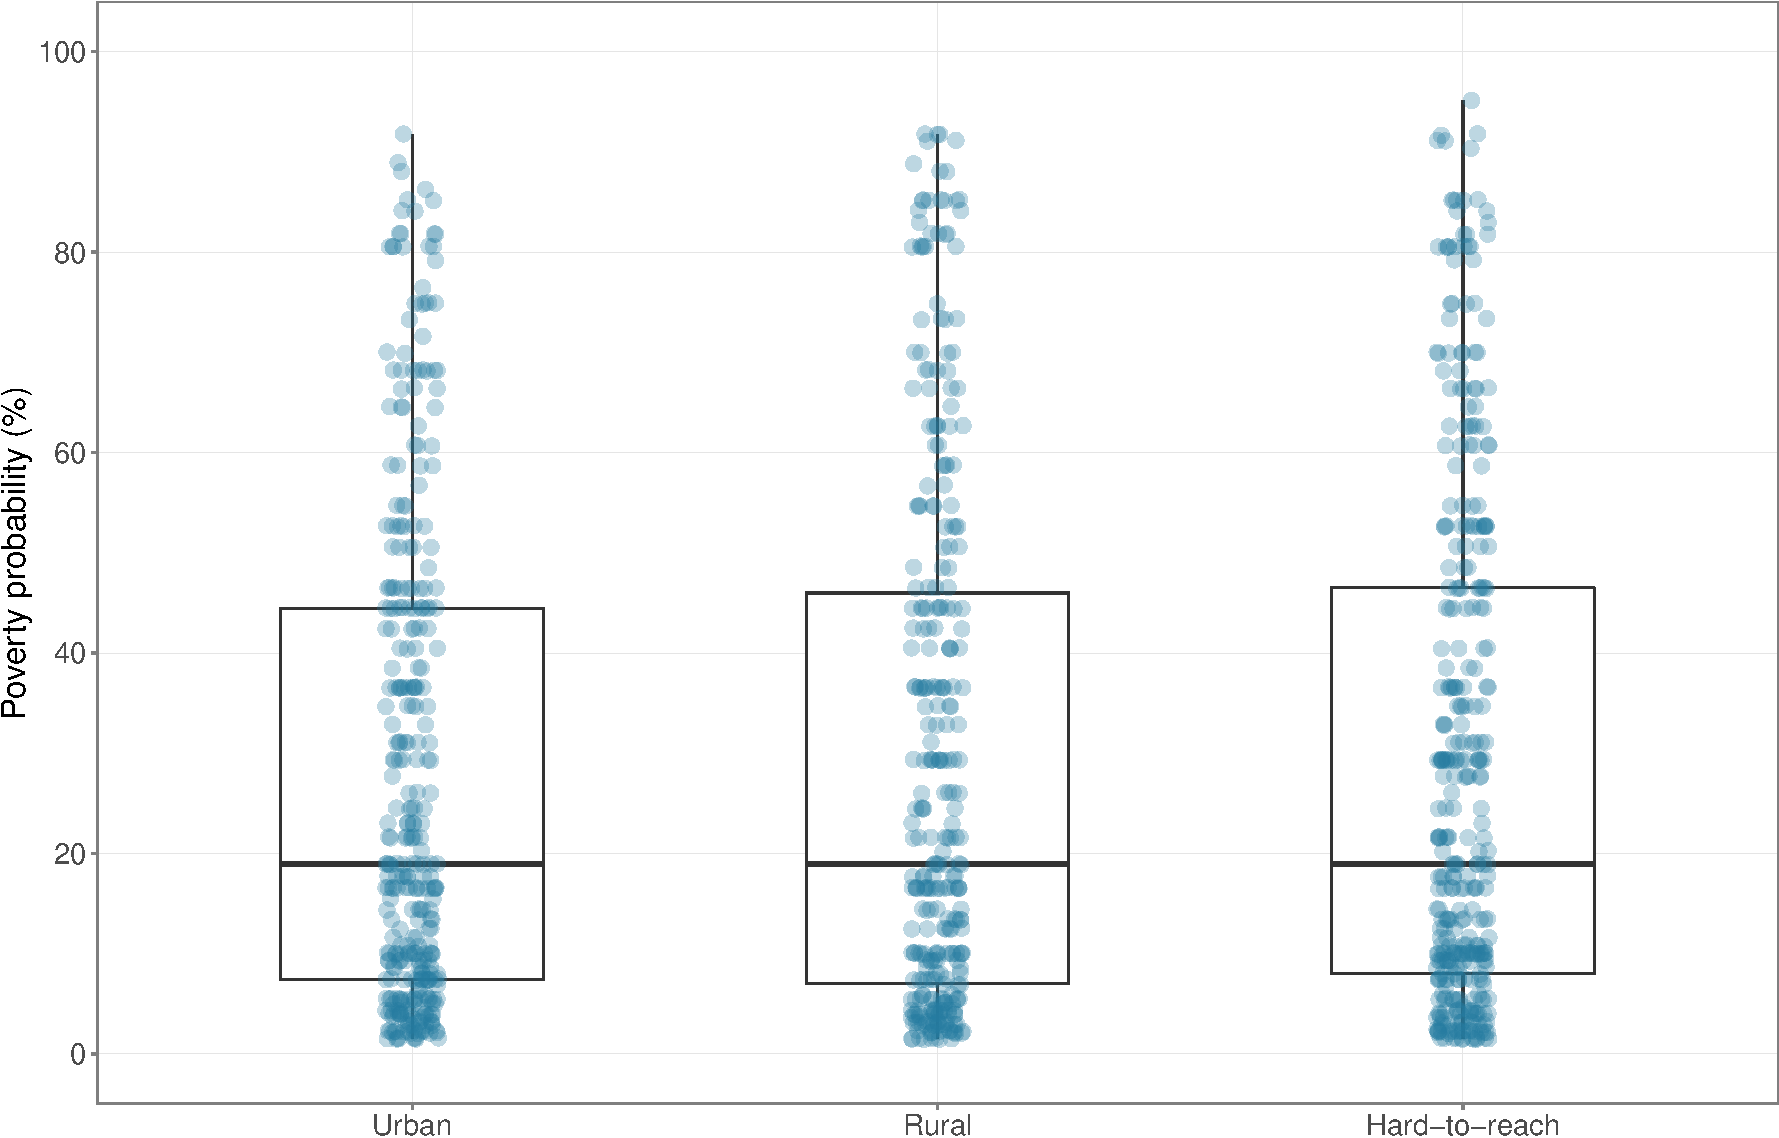
\includegraphics{kayahReport_files/figure-latex/ppiTable-1} 

}

\caption{Poverty probability index by location type}\label{fig:ppiTable}
\end{figure}

\hypertarget{fcs-results}{%
\subsubsection{Food consumption score}\label{fcs-results}}

\begin{table}[H]

\caption{\label{tab:fcs1table}Food consumption score}
\centering
\fontsize{12}{14}\selectfont
\begin{tabular}[t]{>{\bfseries}l>{\bfseries}l>{\ttfamily}r>{\ttfamily}r>{\ttfamily}r>{\ttfamily}r}
\toprule
 &  & \makecell[c]{Mean\\food\\consumption\\score} & \makecell[c]{Poor\\(\%)} & \makecell[c]{Borderline\\(\%)} & \makecell[c]{Acceptable\\(\%)}\\
\midrule
\addlinespace[0.3em]
\multicolumn{6}{l}{\textbf{Kayah}}\\
\addlinespace[0.3em]
\multicolumn{6}{l}{\textit{\textbf{Geographic}}}\\
\hspace{1em}\hspace{1em} & Rural & 60.0 & 1.4 & 5.2 & 93.4\\
\cmidrule{2-6}
\hspace{1em}\hspace{1em} & Urban & 66.9 & 1.6 & 1.8 & 96.5\\
\cmidrule{2-6}
\hspace{1em}\hspace{1em} & Hard-to-reach & 45.9 & 6.6 & 30.2 & 63.2\\
\cmidrule{2-6}
\addlinespace[0.3em]
\multicolumn{6}{l}{\textit{\textbf{Wealth}}}\\
\hspace{1em}\hspace{1em} & Wealthiest & 69.0 & 0.5 & 1.0 & 98.6\\
\cmidrule{2-6}
\hspace{1em}\hspace{1em} & Wealthy & 66.0 & 0.0 & 2.2 & 97.8\\
\cmidrule{2-6}
\hspace{1em}\hspace{1em} & Medium & 59.5 & 1.8 & 8.8 & 89.4\\
\cmidrule{2-6}
\hspace{1em}\hspace{1em} & Poor & 55.2 & 3.2 & 14.9 & 81.9\\
\cmidrule{2-6}
\hspace{1em}\hspace{1em} & Poorest & 42.2 & 7.2 & 32.7 & 60.1\\
\bottomrule
\end{tabular}
\end{table}

\begin{figure}[H]

{\centering 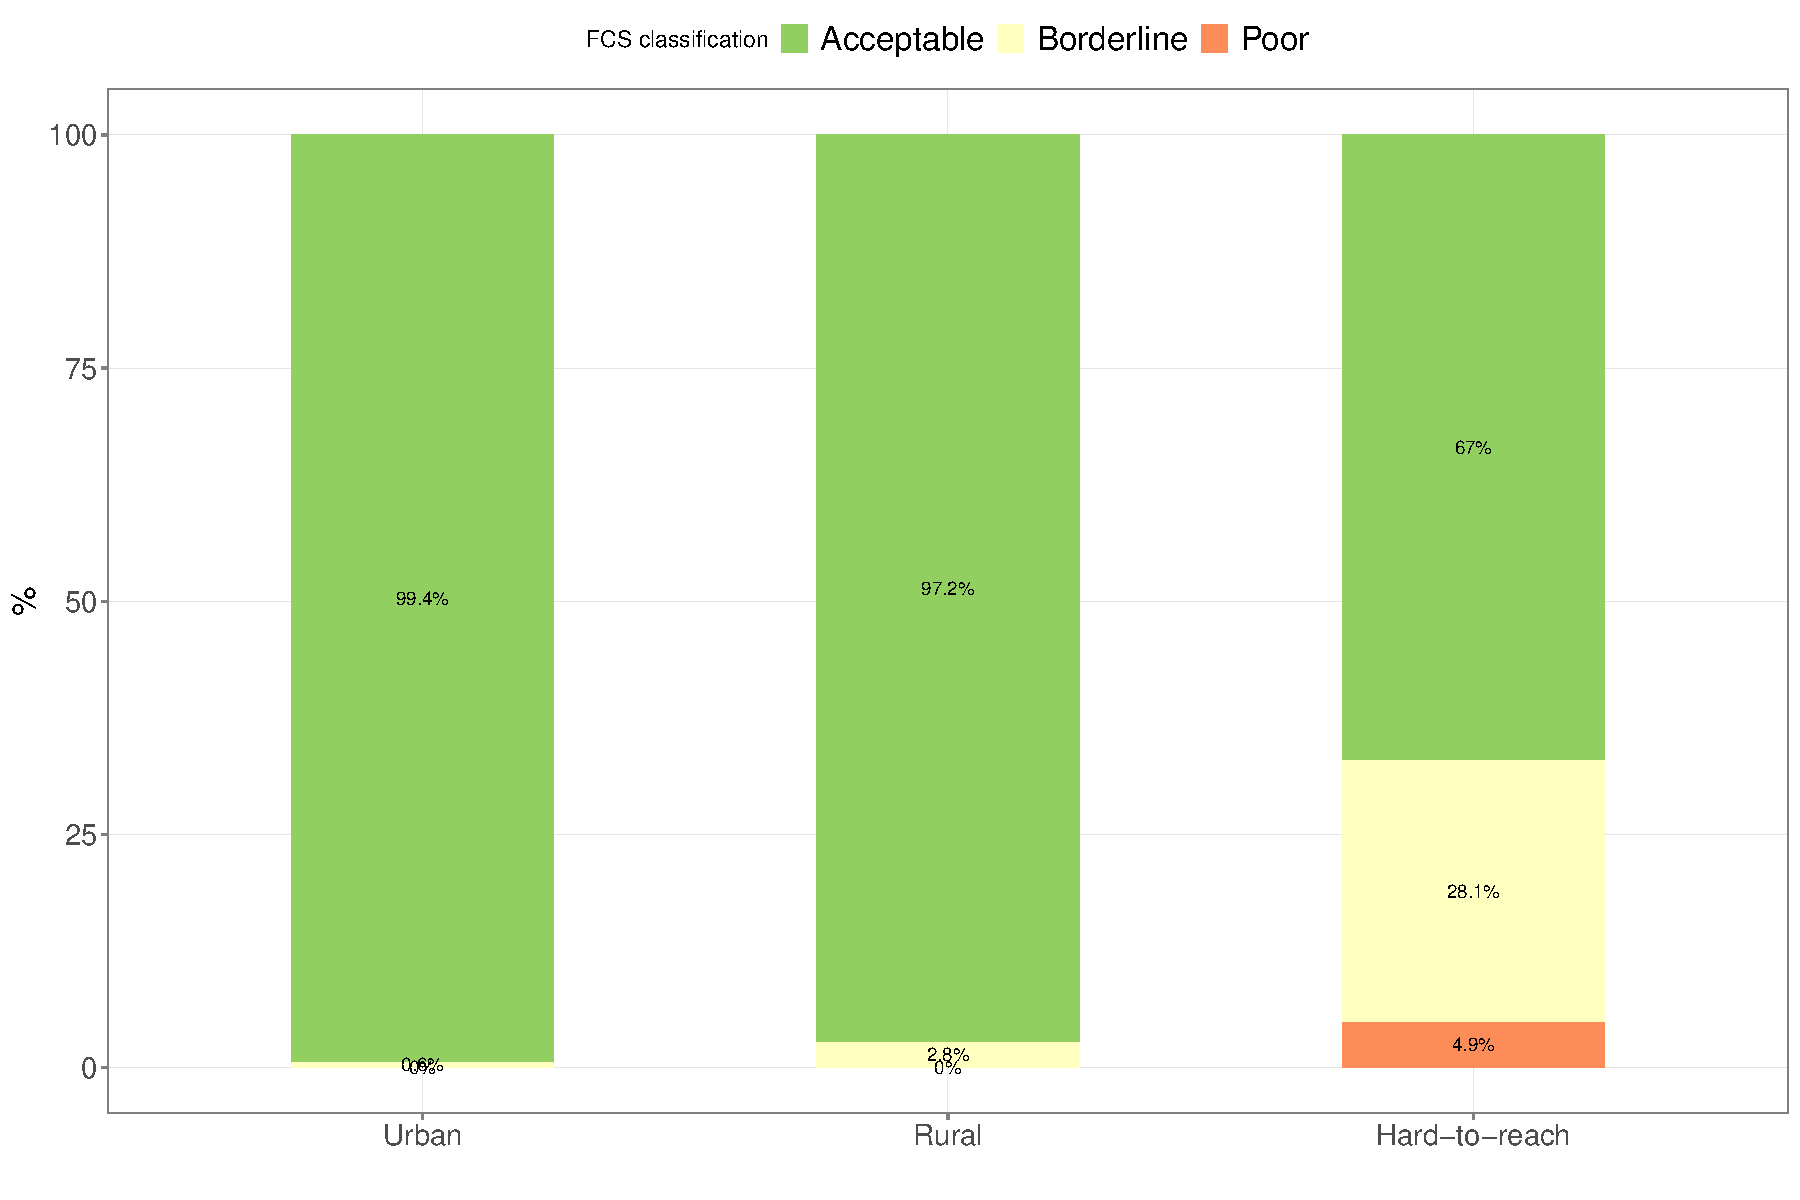
\includegraphics{kayahReport_files/figure-latex/fcs1plot-1} 

}

\caption{Food consumption score classification by location type}\label{fig:fcs1plot}
\end{figure}

\begin{figure}[H]

{\centering 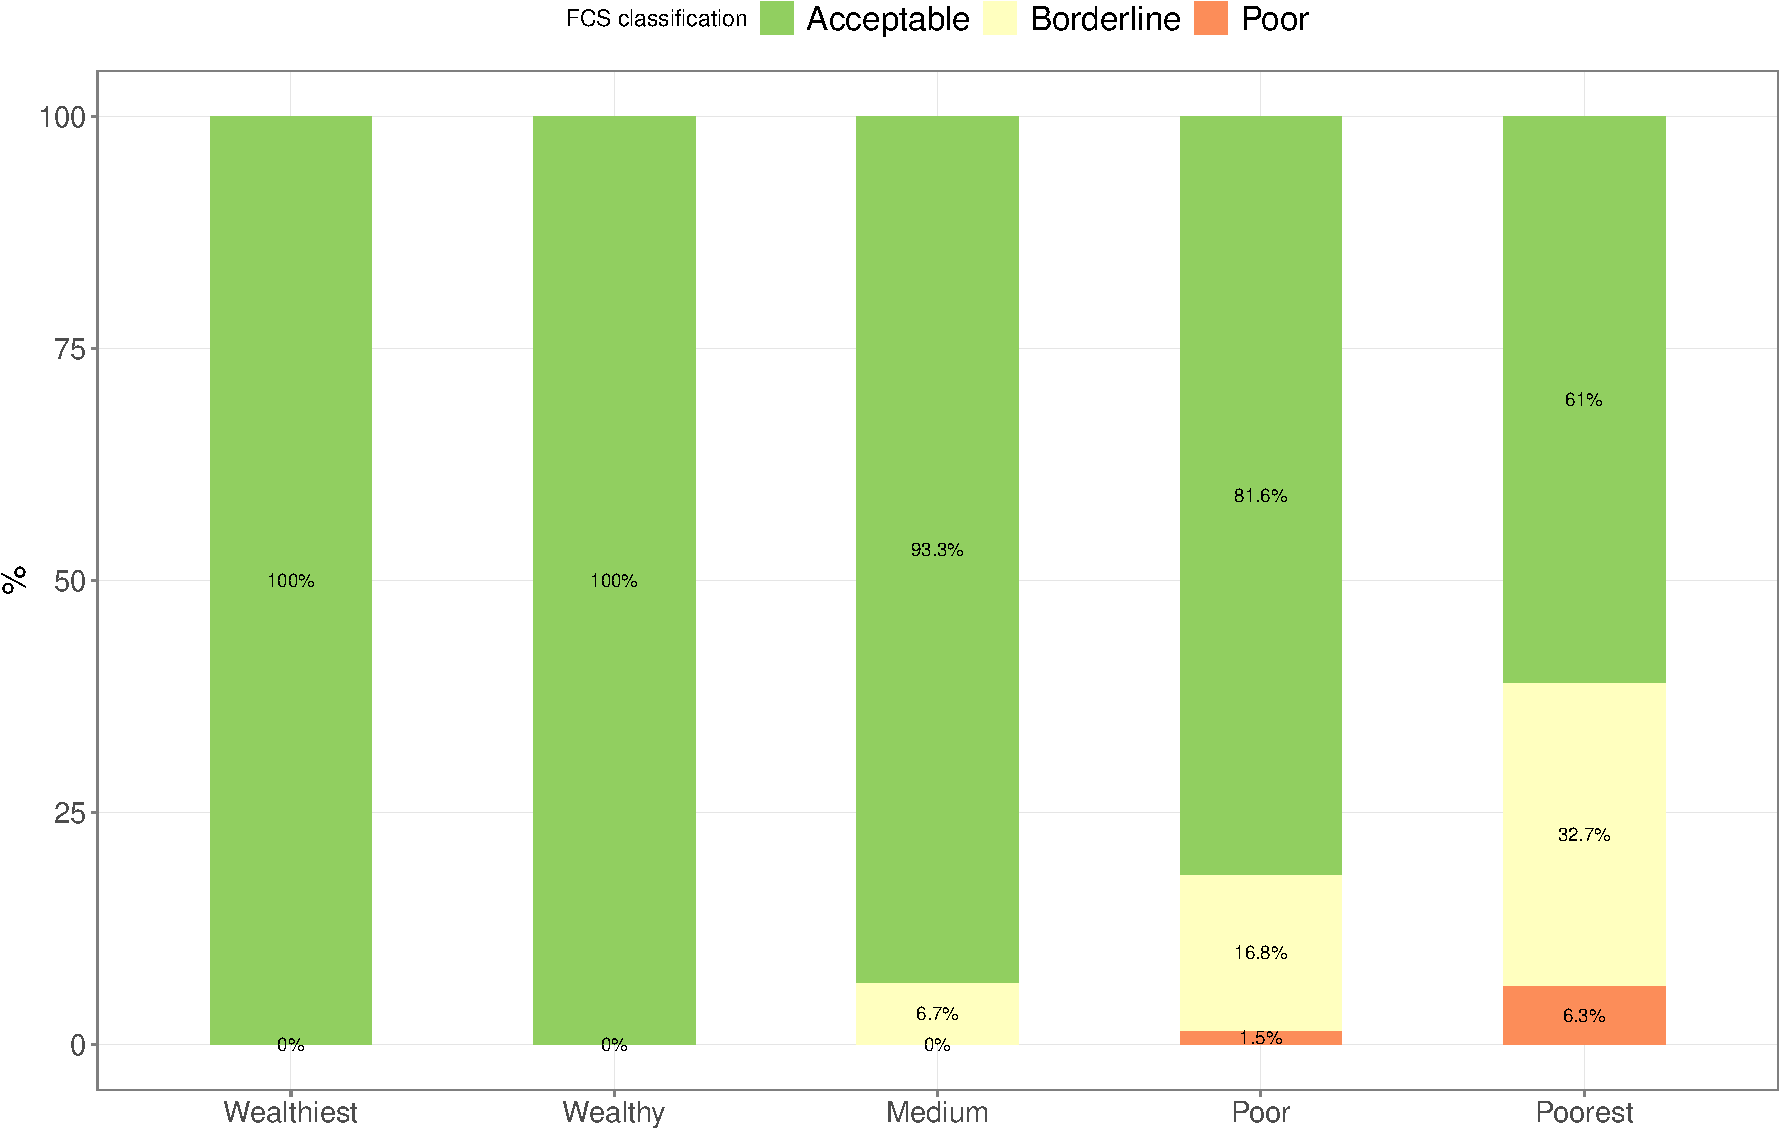
\includegraphics{kayahReport_files/figure-latex/fcs2plot-1} 

}

\caption{Food consumption score classification by wealth quintiles}\label{fig:fcs2plot}
\end{figure}

\hypertarget{fcsn-results}{%
\subsubsection{Food consumption score - nutrition}\label{fcsn-results}}

\begin{landscape}\begin{table}[H]

\caption{\label{tab:fcsn1table}Food consumption score - nutrition}
\centering
\fontsize{10}{12}\selectfont
\begin{tabular}[t]{>{\bfseries}l>{\bfseries}l>{\ttfamily}r>{\ttfamily}r>{\ttfamily}r>{\ttfamily}r>{\ttfamily}r>{\ttfamily}r>{\ttfamily}r>{\ttfamily}r>{\ttfamily}r}
\toprule
\multicolumn{2}{c}{ } & \multicolumn{3}{c}{Vitamin A-rich foods} & \multicolumn{3}{c}{Protein-rich foods} & \multicolumn{3}{c}{Heme iron-rich foods} \\
\cmidrule(l{3pt}r{3pt}){3-5} \cmidrule(l{3pt}r{3pt}){6-8} \cmidrule(l{3pt}r{3pt}){9-11}
 &  & \makecell[c]{Never\\(\%)} & \makecell[c]{Sometimes\\(\%)} & \makecell[c]{At\\least\\daily\\(\%)} & \makecell[c]{Never\\(\%)} & \makecell[c]{Sometimes\\(\%)} & \makecell[c]{At\\least\\daily\\(\%)} & \makecell[c]{Never\\(\%)} & \makecell[c]{Sometimes\\(\%)} & \makecell[c]{At\\least\\daily\\(\%)}\\
\midrule
\addlinespace[0.3em]
\multicolumn{11}{l}{\textbf{Kayah}}\\
\addlinespace[0.3em]
\multicolumn{11}{l}{\textit{\textbf{Geographic}}}\\
\hspace{1em}\hspace{1em} & Rural & 4.6 & 21.9 & 73.5 & 1.4 & 20.2 & 78.4 & 5.2 & 46.4 & 48.4\\
\cmidrule{2-11}
\hspace{1em}\hspace{1em} & Urban & 1.8 & 16.4 & 81.8 & 1.8 & 8.8 & 89.4 & 2.3 & 44.6 & 53.1\\
\cmidrule{2-11}
\hspace{1em}\hspace{1em} & Hard-to-reach & 10.0 & 31.6 & 58.4 & 9.7 & 47.9 & 42.5 & 16.8 & 63.2 & 19.9\\
\cmidrule{2-11}
\addlinespace[0.3em]
\multicolumn{11}{l}{\textit{\textbf{Wealth}}}\\
\hspace{1em}\hspace{1em} & Wealthiest & 1.0 & 14.4 & 84.7 & 1.0 & 7.2 & 91.9 & 1.0 & 40.2 & 58.9\\
\cmidrule{2-11}
\hspace{1em}\hspace{1em} & Wealthy & 0.0 & 17.7 & 82.3 & 0.0 & 13.0 & 87.0 & 0.4 & 50.6 & 48.9\\
\cmidrule{2-11}
\hspace{1em}\hspace{1em} & Medium & 2.3 & 23.5 & 74.2 & 1.8 & 23.0 & 75.1 & 4.1 & 55.8 & 40.1\\
\cmidrule{2-11}
\hspace{1em}\hspace{1em} & Poor & 5.0 & 24.0 & 71.0 & 3.6 & 28.5 & 67.9 & 10.4 & 52.9 & 36.7\\
\cmidrule{2-11}
\hspace{1em}\hspace{1em} & Poorest & 15.2 & 36.3 & 48.4 & 11.7 & 52.9 & 35.4 & 20.2 & 58.3 & 21.5\\
\bottomrule
\end{tabular}
\end{table}
\end{landscape}

\begin{figure}[H]

{\centering 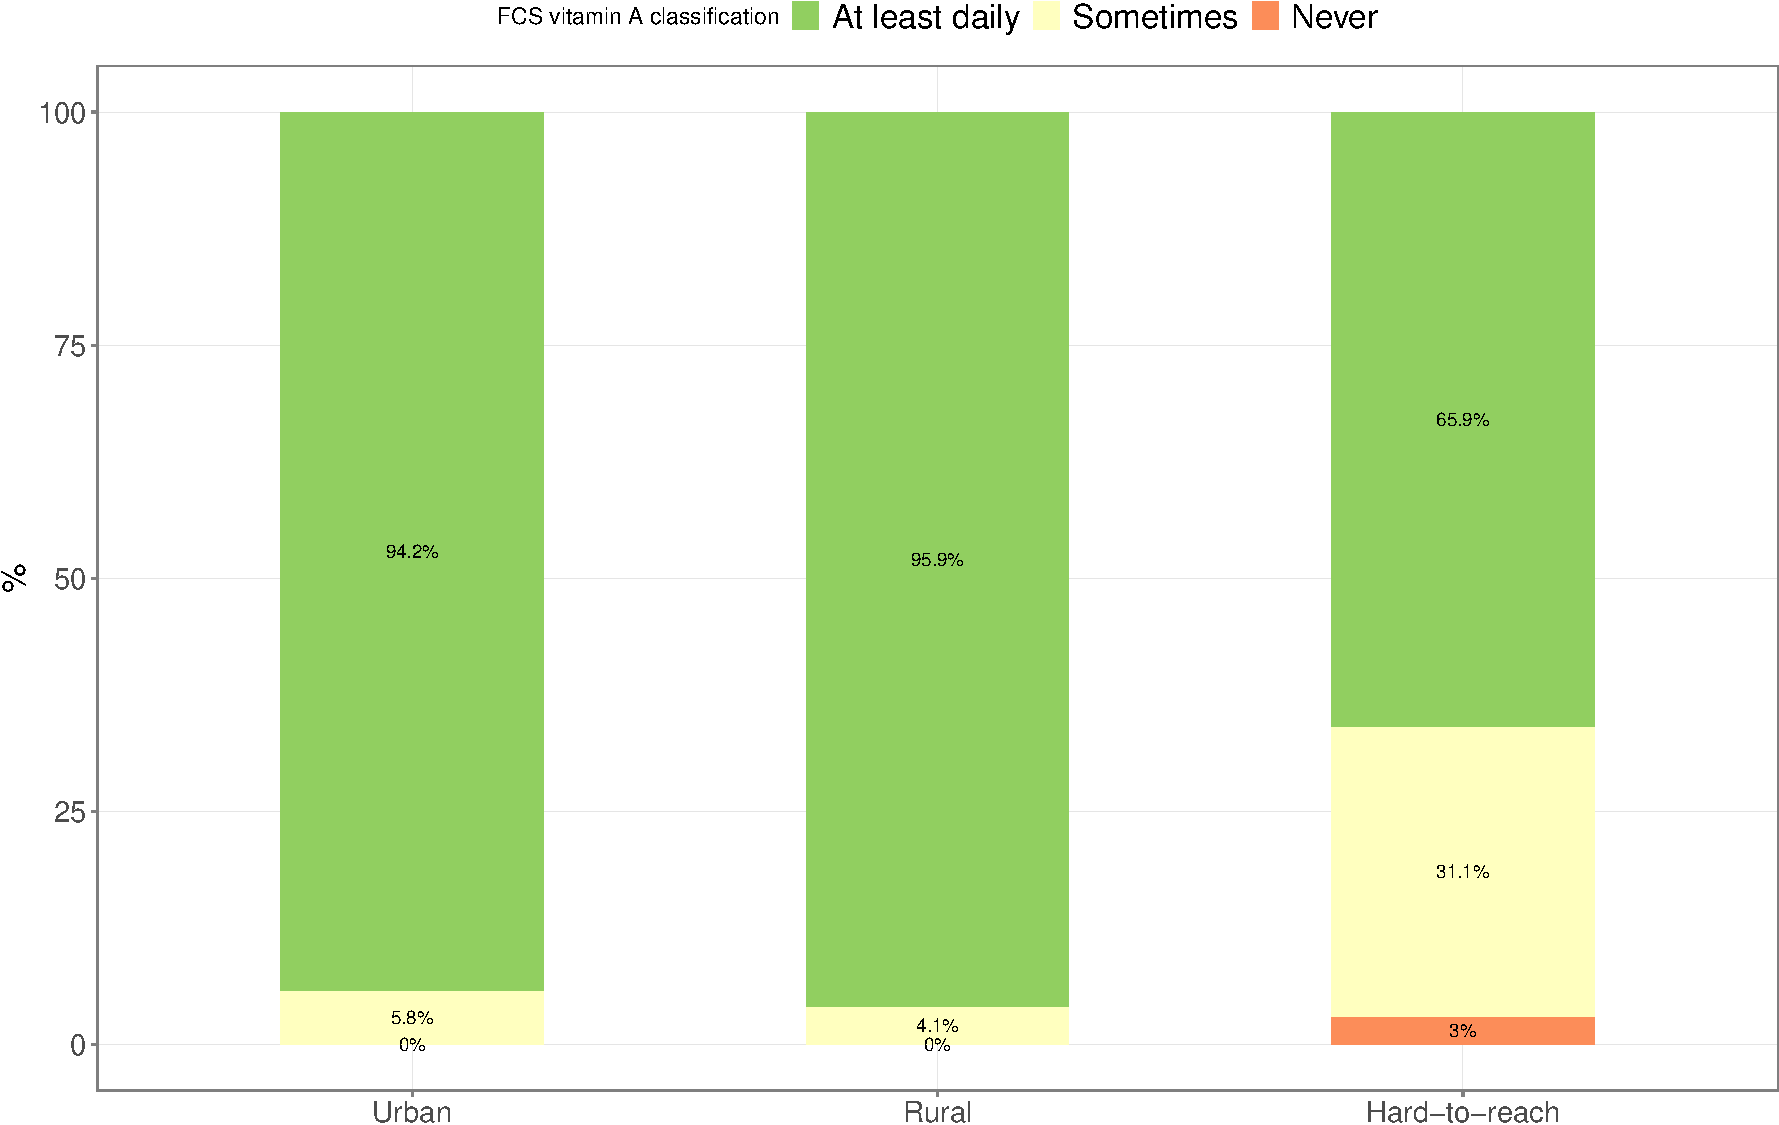
\includegraphics{kayahReport_files/figure-latex/fcsn1plot-1} 

}

\caption{Vitamin A food consumption score classification by location type}\label{fig:fcsn1plot}
\end{figure}

\begin{figure}[H]

{\centering 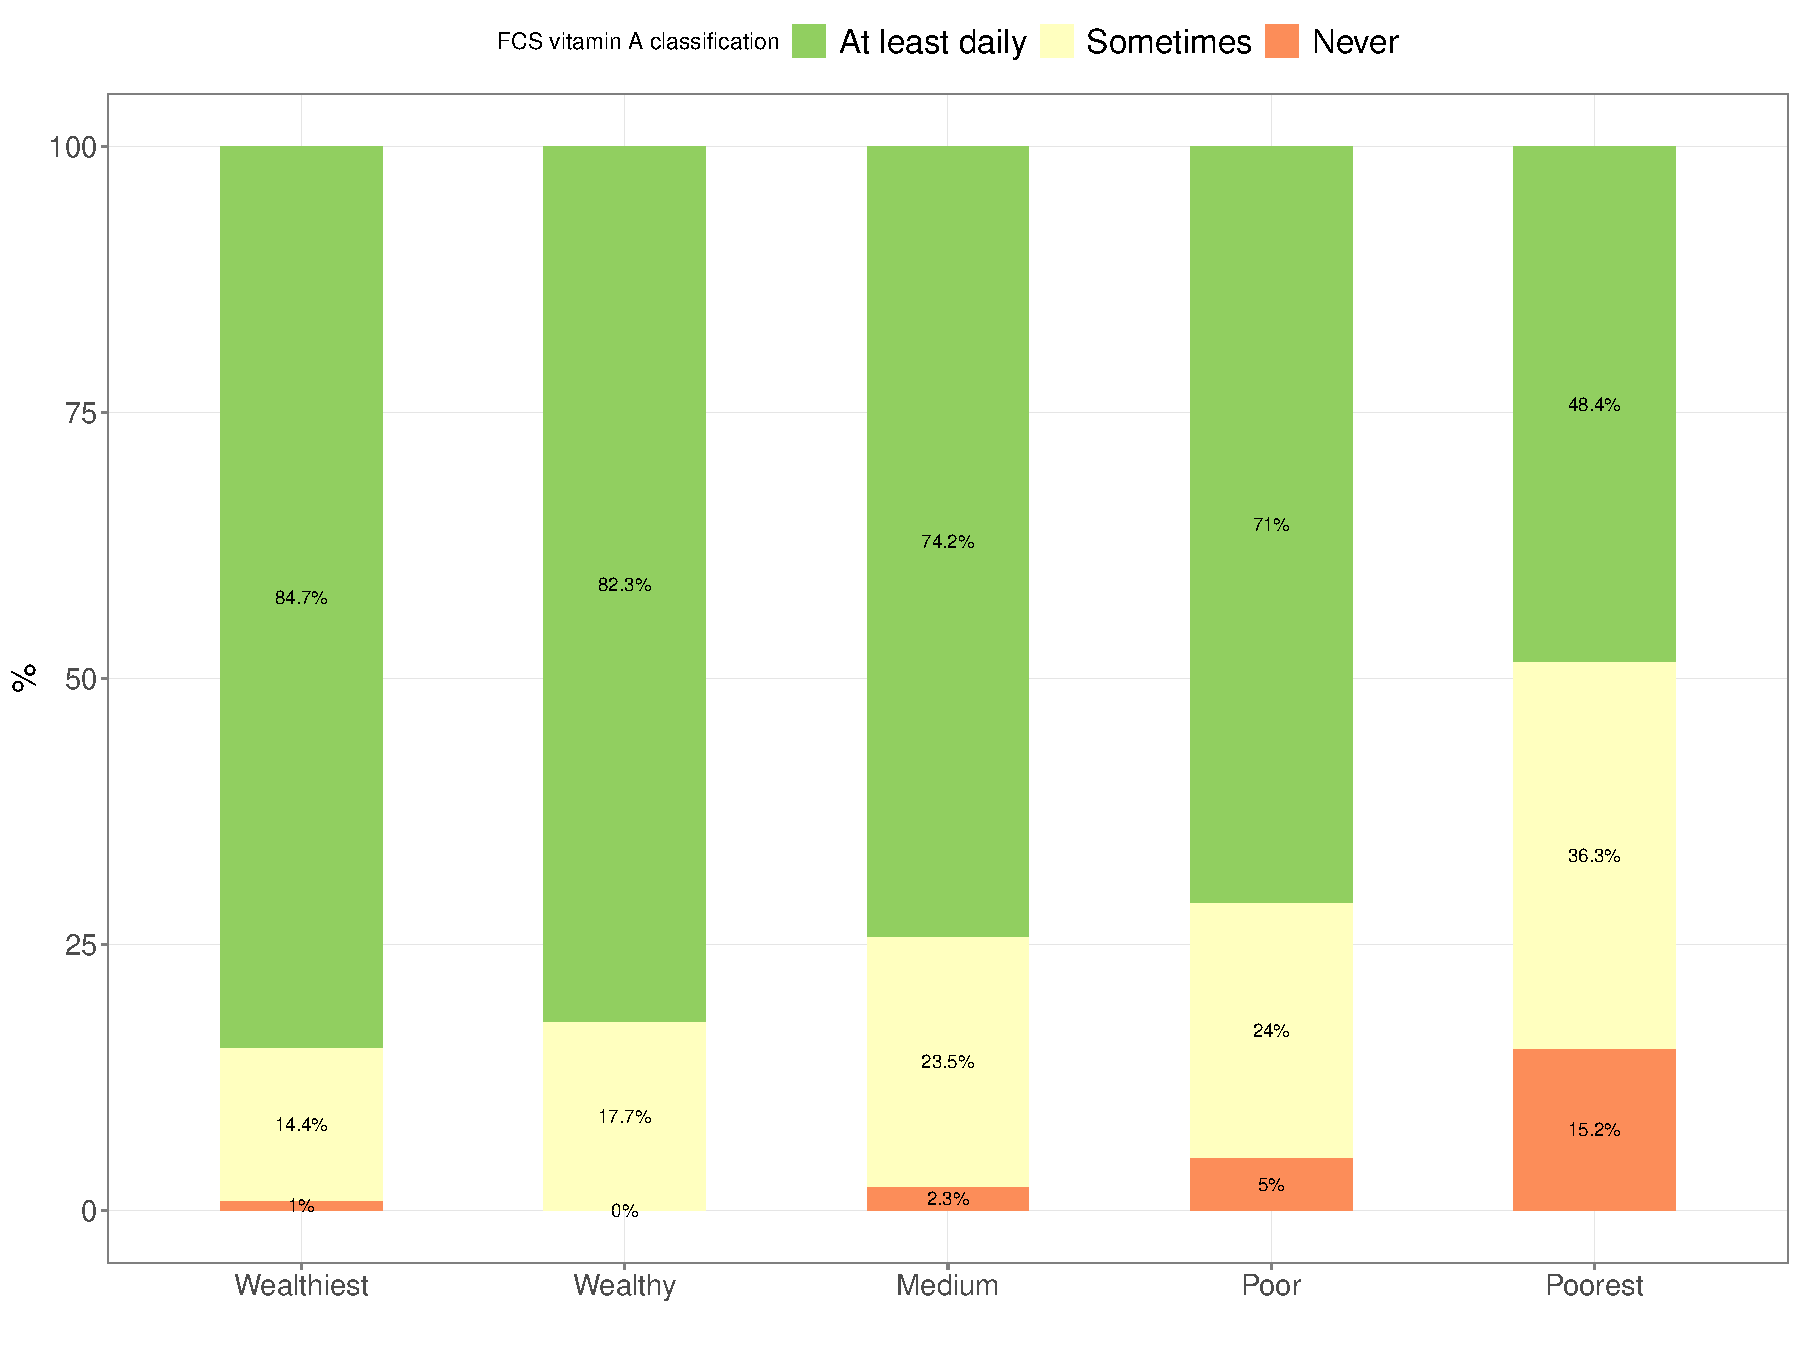
\includegraphics{kayahReport_files/figure-latex/fcsn2plot-1} 

}

\caption{Vitamin A food consumption score classification by wealth quintiles}\label{fig:fcsn2plot}
\end{figure}

\begin{figure}[H]

{\centering 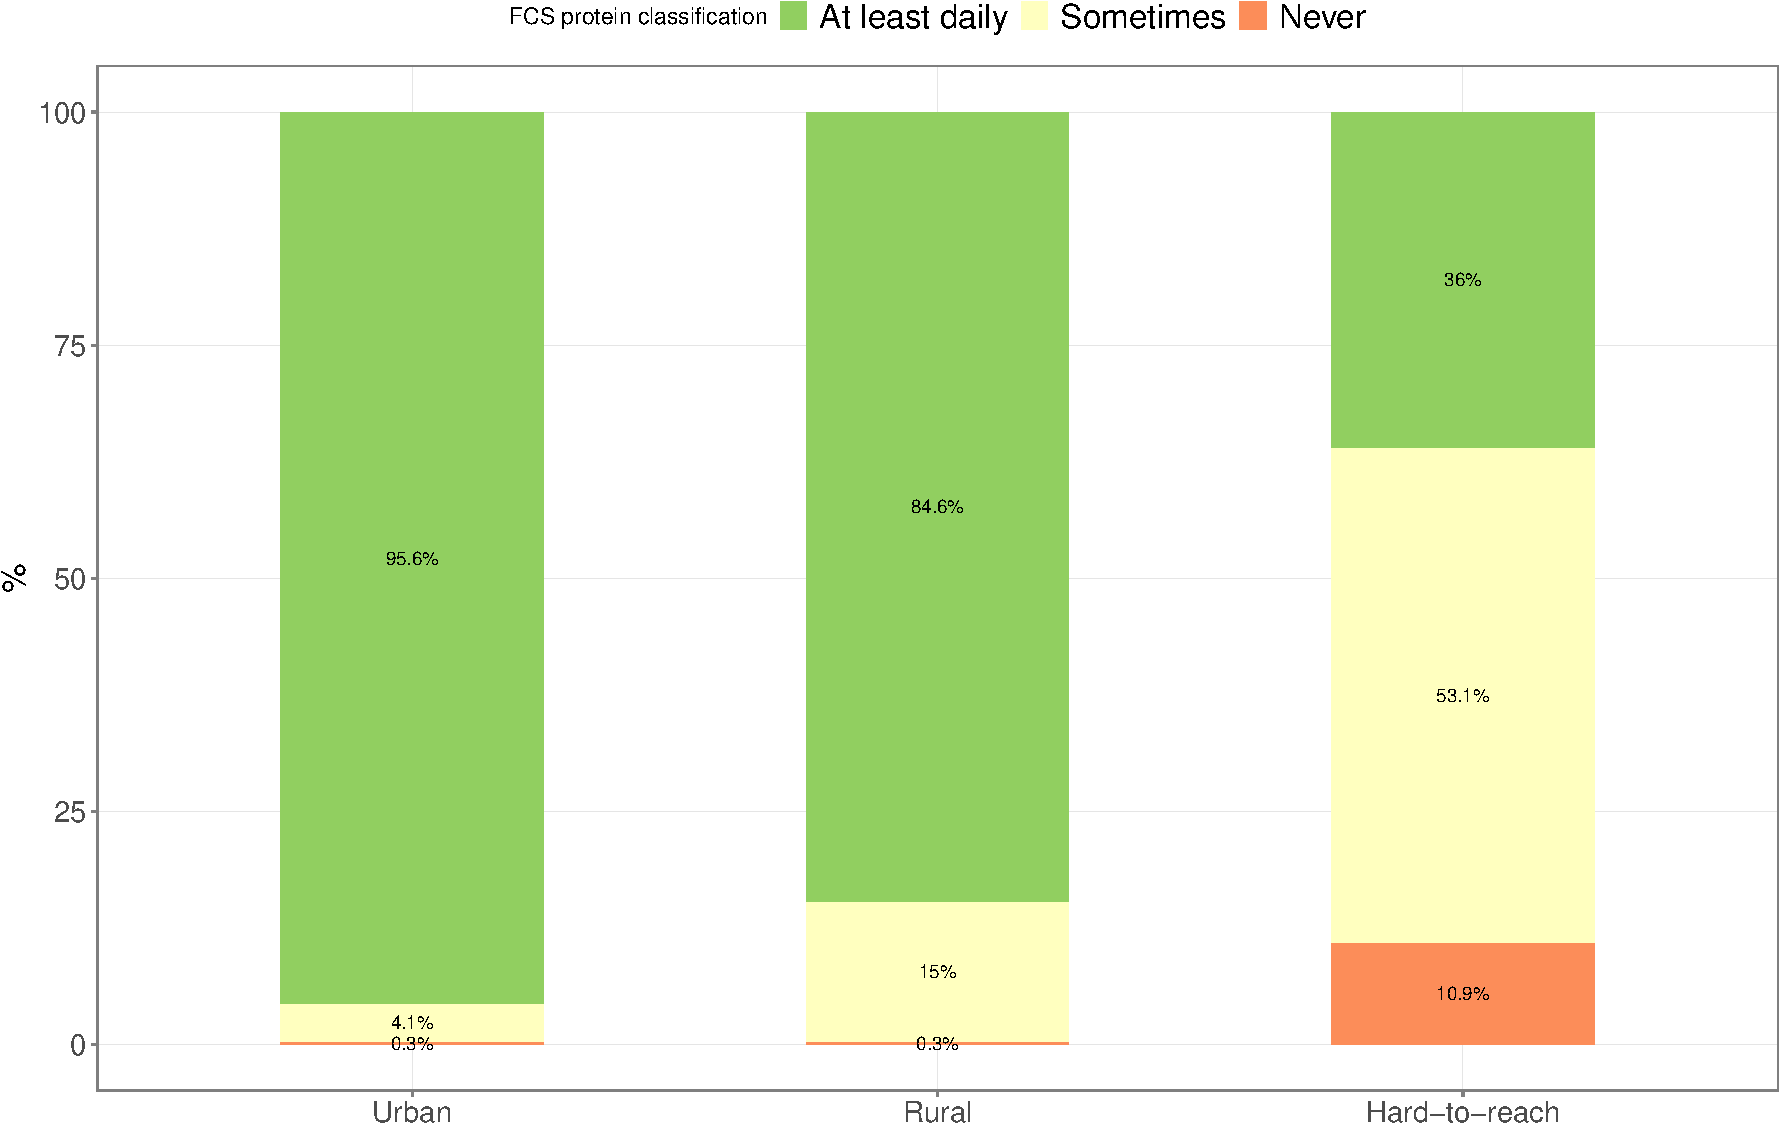
\includegraphics{kayahReport_files/figure-latex/fcsn3plot-1} 

}

\caption{Protein food consumption score classification by location type}\label{fig:fcsn3plot}
\end{figure}

\begin{figure}[H]

{\centering 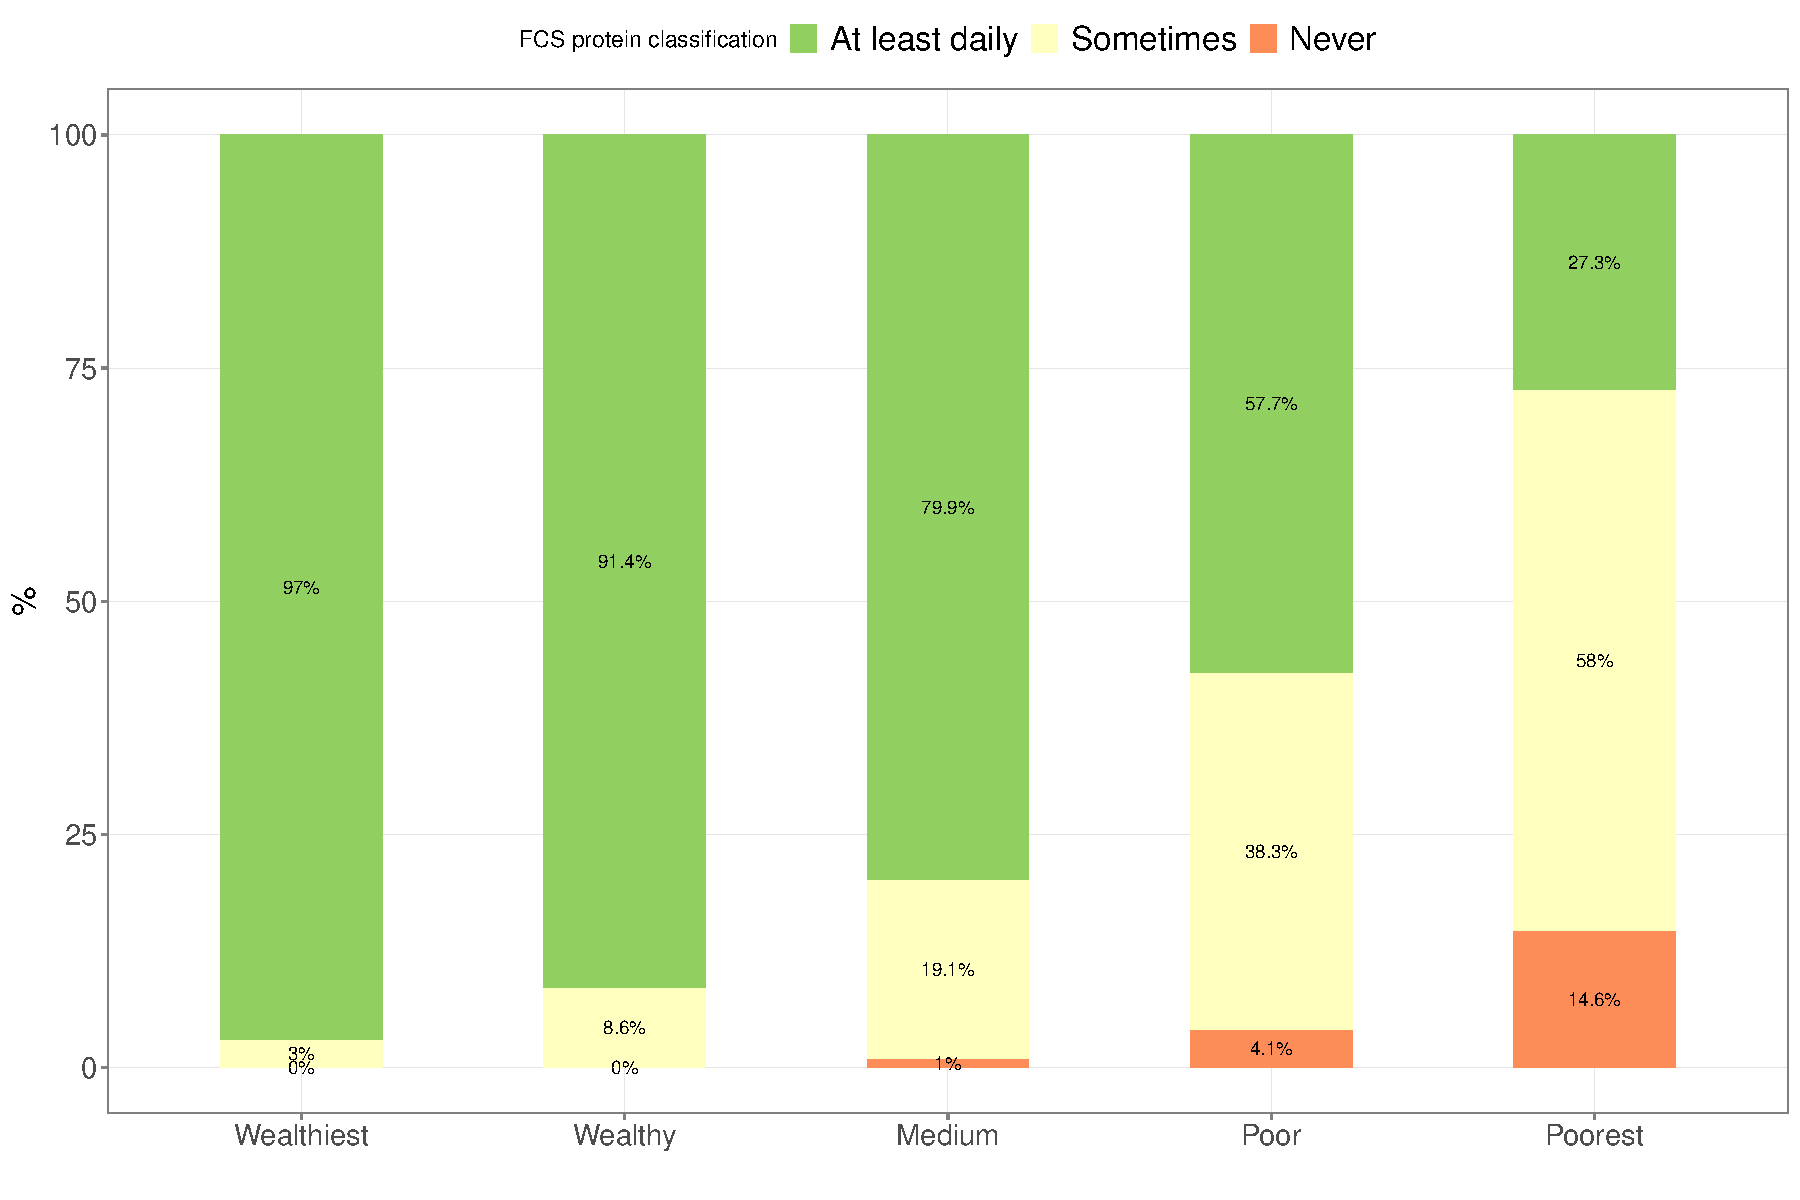
\includegraphics{kayahReport_files/figure-latex/fcsn4plot-1} 

}

\caption{Protein food consumption score classification by wealth quintiles}\label{fig:fcsn4plot}
\end{figure}

\hypertarget{csi-results}{%
\subsubsection{Coping strategies index}\label{csi-results}}

\hypertarget{ccsi-results}{%
\paragraph{Consumption-based coping strategies index}\label{ccsi-results}}

\begin{table}[H]

\caption{\label{tab:ccsi1table}Consumption-based Coping Strategies Index}
\centering
\fontsize{12}{14}\selectfont
\begin{tabular}[t]{>{\bfseries}l>{\bfseries}l>{\ttfamily}r}
\toprule
 &  & Mean CSI\\
\midrule
\addlinespace[0.3em]
\multicolumn{3}{l}{\textbf{Kayah}}\\
\addlinespace[0.3em]
\multicolumn{3}{l}{\textit{\textbf{Geographic}}}\\
\hspace{1em}\hspace{1em} & Rural & 3.0\\
\cmidrule{2-3}
\hspace{1em}\hspace{1em} & Urban & 2.8\\
\cmidrule{2-3}
\hspace{1em}\hspace{1em} & Hard-to-reach & 3.2\\
\cmidrule{2-3}
\addlinespace[0.3em]
\multicolumn{3}{l}{\textit{\textbf{Wealth}}}\\
\hspace{1em}\hspace{1em} & Wealthiest & 2.0\\
\cmidrule{2-3}
\hspace{1em}\hspace{1em} & Wealthy & 2.1\\
\cmidrule{2-3}
\hspace{1em}\hspace{1em} & Medium & 2.7\\
\cmidrule{2-3}
\hspace{1em}\hspace{1em} & Poor & 3.3\\
\cmidrule{2-3}
\hspace{1em}\hspace{1em} & Poorest & 5.2\\
\bottomrule
\end{tabular}
\end{table}

\begin{figure}[H]

{\centering 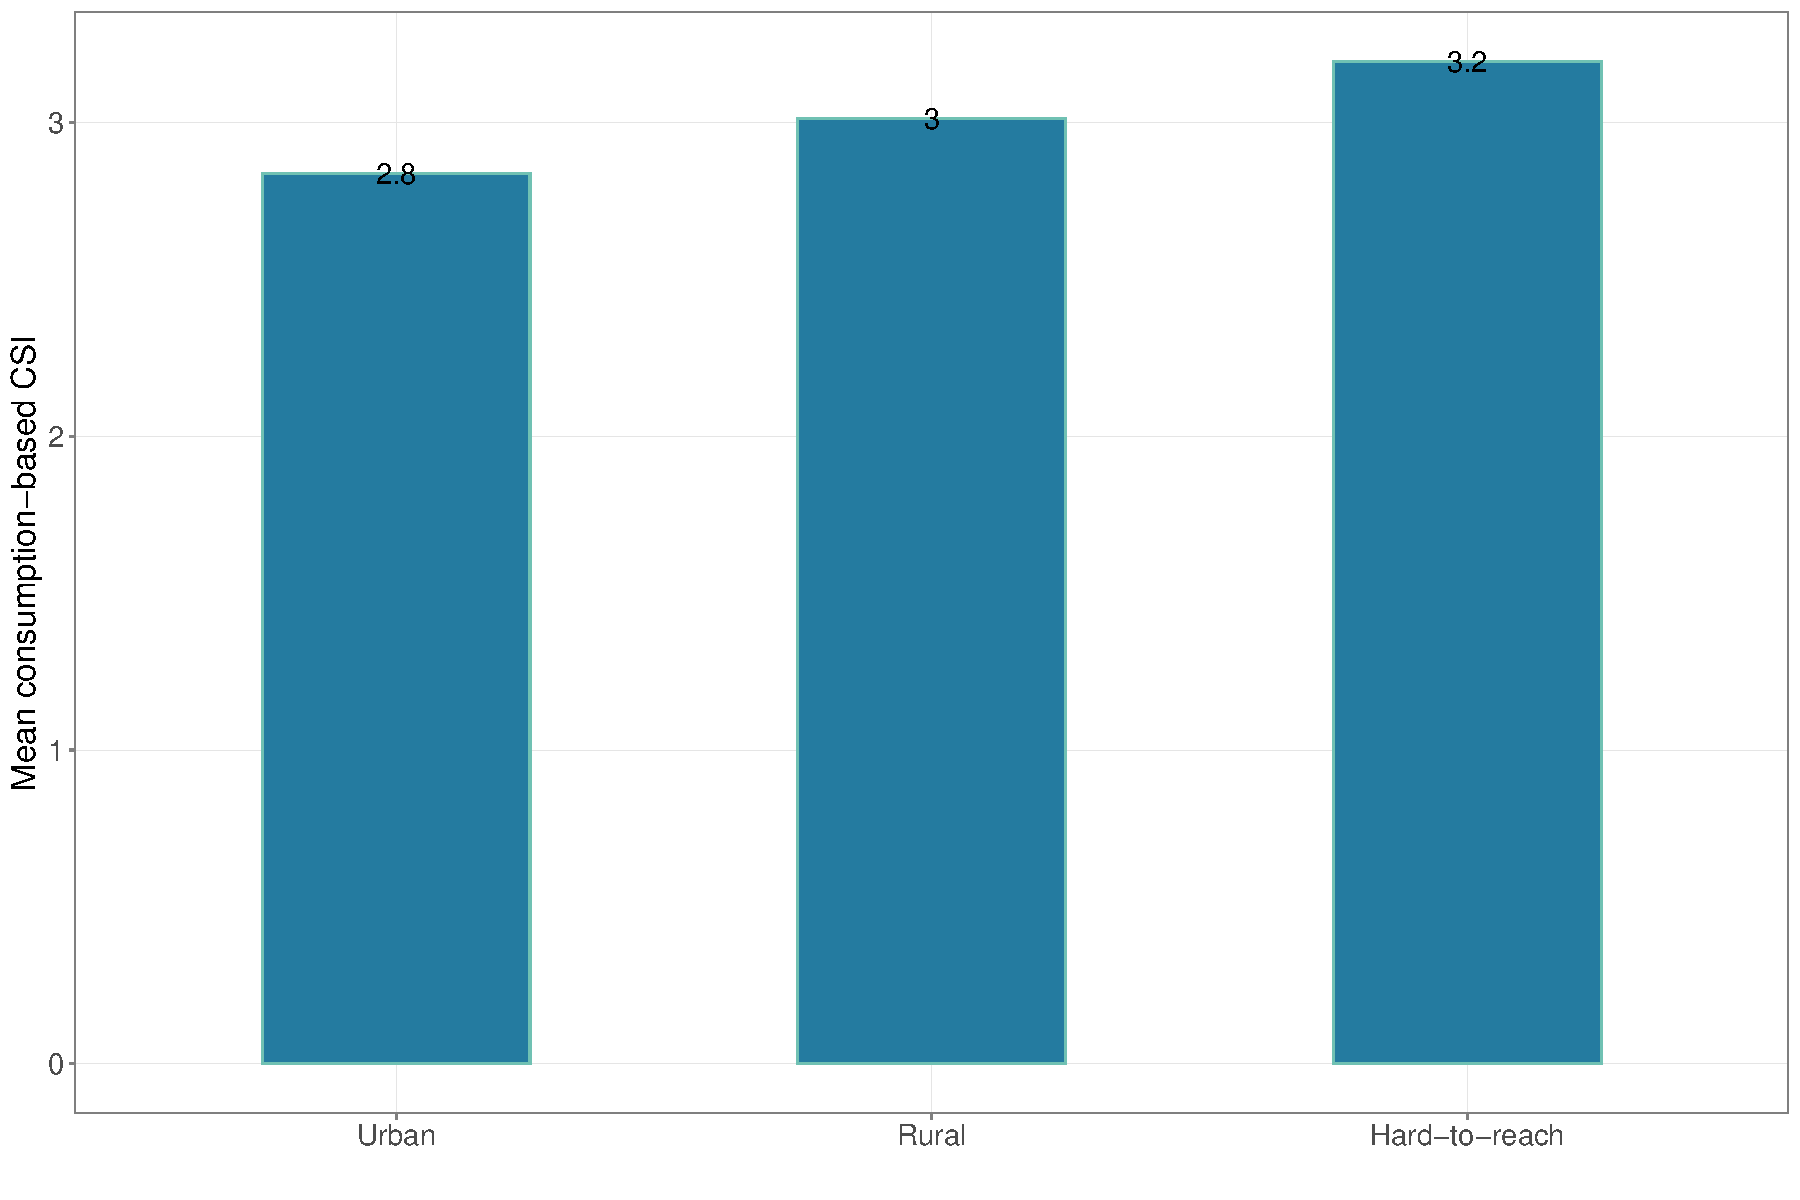
\includegraphics{kayahReport_files/figure-latex/ccsi1plot-1} 

}

\caption{Consumption-based coping strategies index by location type}\label{fig:ccsi1plot}
\end{figure}

\begin{figure}[H]

{\centering 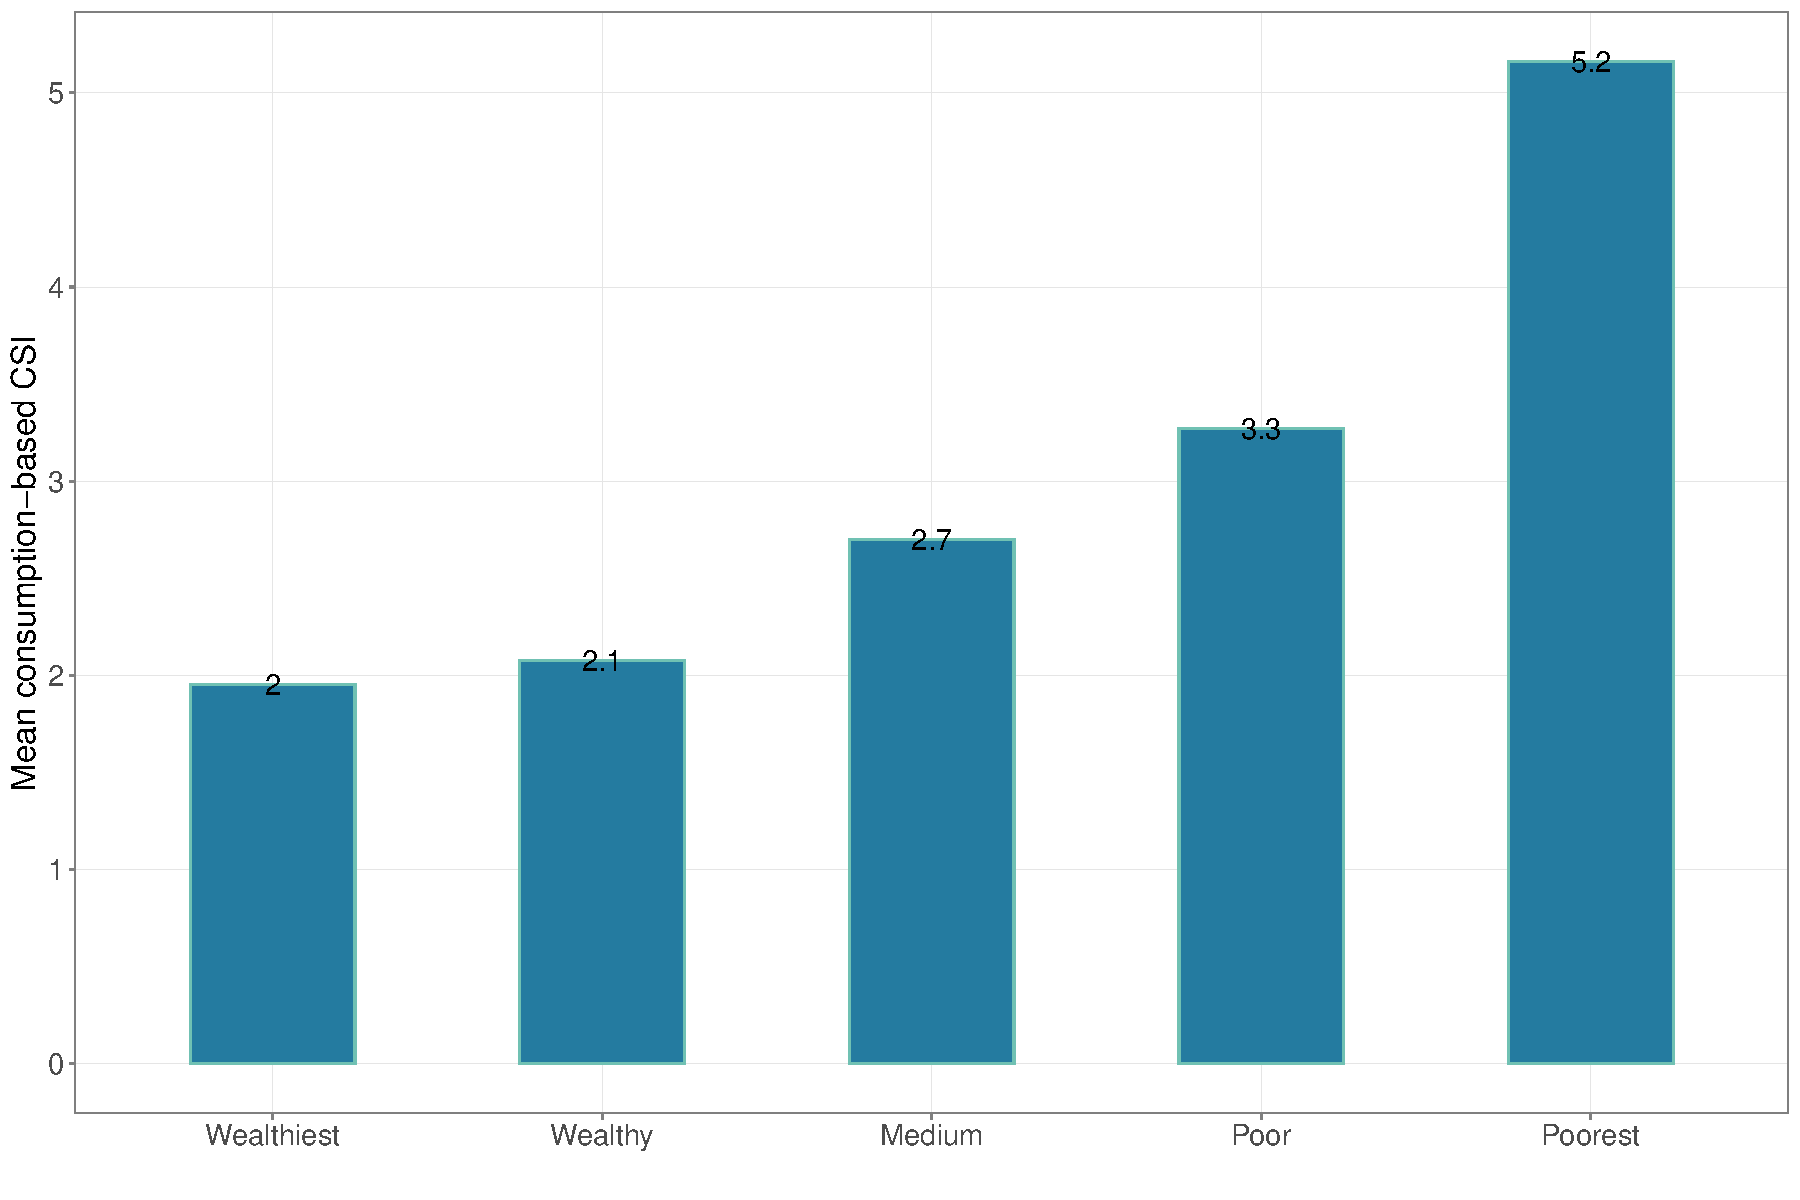
\includegraphics{kayahReport_files/figure-latex/ccsi2plot-1} 

}

\caption{Consumption-based coping strategies index by wealth quintiles}\label{fig:ccsi2plot}
\end{figure}

\hypertarget{lcsi-results}{%
\paragraph{Livelihood-based coping strategies index}\label{lcsi-results}}

\begin{table}[H]

\caption{\label{tab:lcsi1table}Livelihoods-based coping strategies index}
\centering
\fontsize{12}{14}\selectfont
\begin{tabular}[t]{>{\bfseries}l>{\bfseries}l>{\ttfamily}r>{\ttfamily}r>{\ttfamily}r>{\ttfamily}r}
\toprule
 &  & \makecell[c]{Secure\\(\%)} & \makecell[c]{Stress\\(\%)} & \makecell[c]{Crisis\\(\%)} & \makecell[c]{Emergency\\(\%)}\\
\midrule
\addlinespace[0.3em]
\multicolumn{6}{l}{\textbf{Kayah}}\\
\addlinespace[0.3em]
\multicolumn{6}{l}{\textit{\textbf{Geographic}}}\\
\hspace{1em}\hspace{1em} & Rural & 46.7 & 39.8 & 11.5 & 2.0\\
\cmidrule{2-6}
\hspace{1em}\hspace{1em} & Urban & 39.7 & 44.6 & 14.8 & 0.9\\
\cmidrule{2-6}
\hspace{1em}\hspace{1em} & Hard-to-reach & 60.4 & 32.2 & 5.4 & 2.0\\
\cmidrule{2-6}
\addlinespace[0.3em]
\multicolumn{6}{l}{\textit{\textbf{Wealth}}}\\
\hspace{1em}\hspace{1em} & Wealthiest & 46.9 & 43.5 & 8.6 & 1.0\\
\cmidrule{2-6}
\hspace{1em}\hspace{1em} & Wealthy & 40.7 & 45.0 & 13.4 & 0.9\\
\cmidrule{2-6}
\hspace{1em}\hspace{1em} & Medium & 47.0 & 38.2 & 13.8 & 0.9\\
\cmidrule{2-6}
\hspace{1em}\hspace{1em} & Poor & 49.3 & 37.1 & 10.9 & 2.7\\
\cmidrule{2-6}
\hspace{1em}\hspace{1em} & Poorest & 55.6 & 33.6 & 8.1 & 2.7\\
\bottomrule
\end{tabular}
\end{table}

\begin{figure}[H]

{\centering 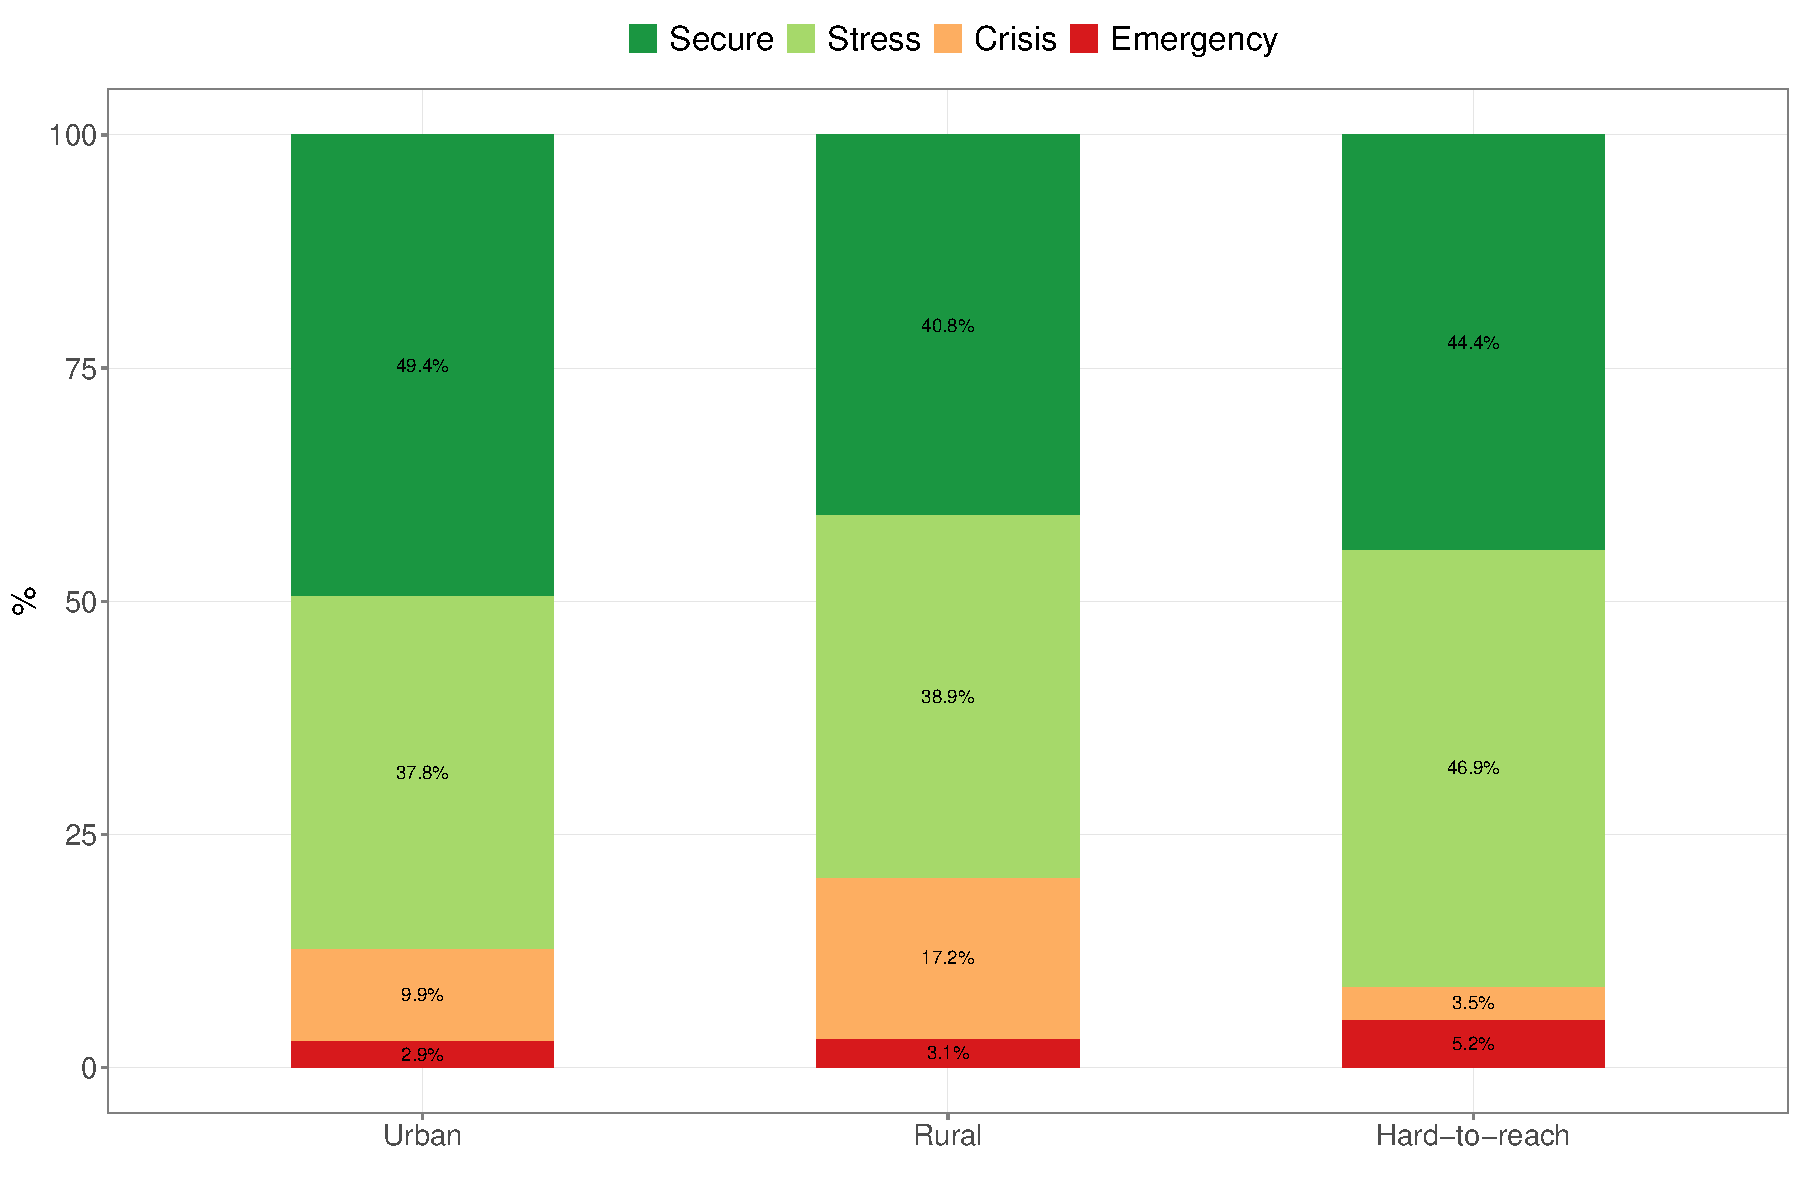
\includegraphics{kayahReport_files/figure-latex/lcsi1plot-1} 

}

\caption{Livelihoods-based coping strategies index by location type}\label{fig:lcsi1plot}
\end{figure}

\begin{figure}[H]

{\centering 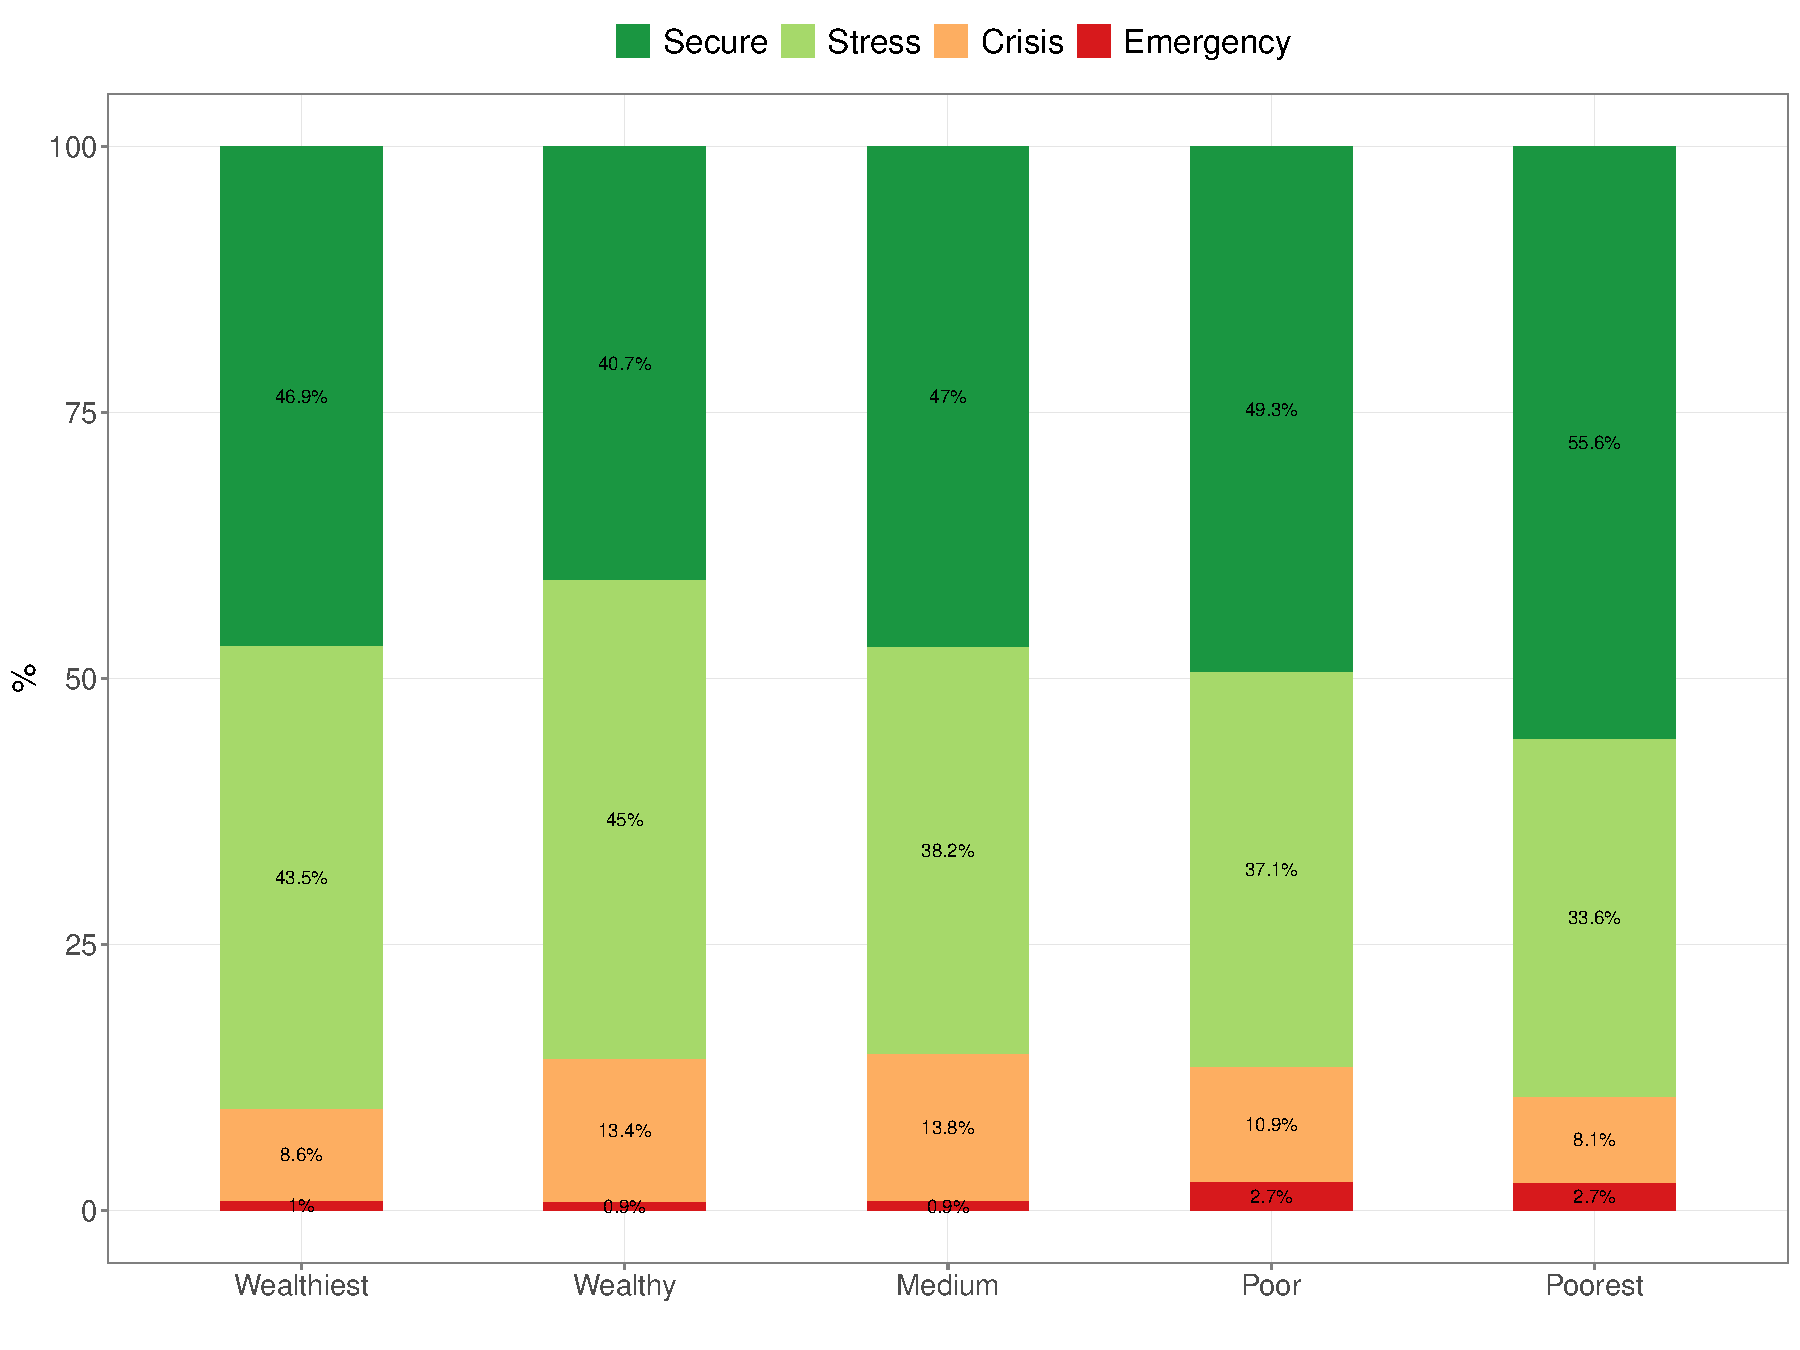
\includegraphics{kayahReport_files/figure-latex/lcsi2plot-1} 

}

\caption{Livelihoods-based coping strategies index by wealth quintiles}\label{fig:lcsi2plot}
\end{figure}

\hypertarget{hfes-results}{%
\subsubsection{Household food expenditure share}\label{hfes-results}}

\begin{figure}[H]

{\centering 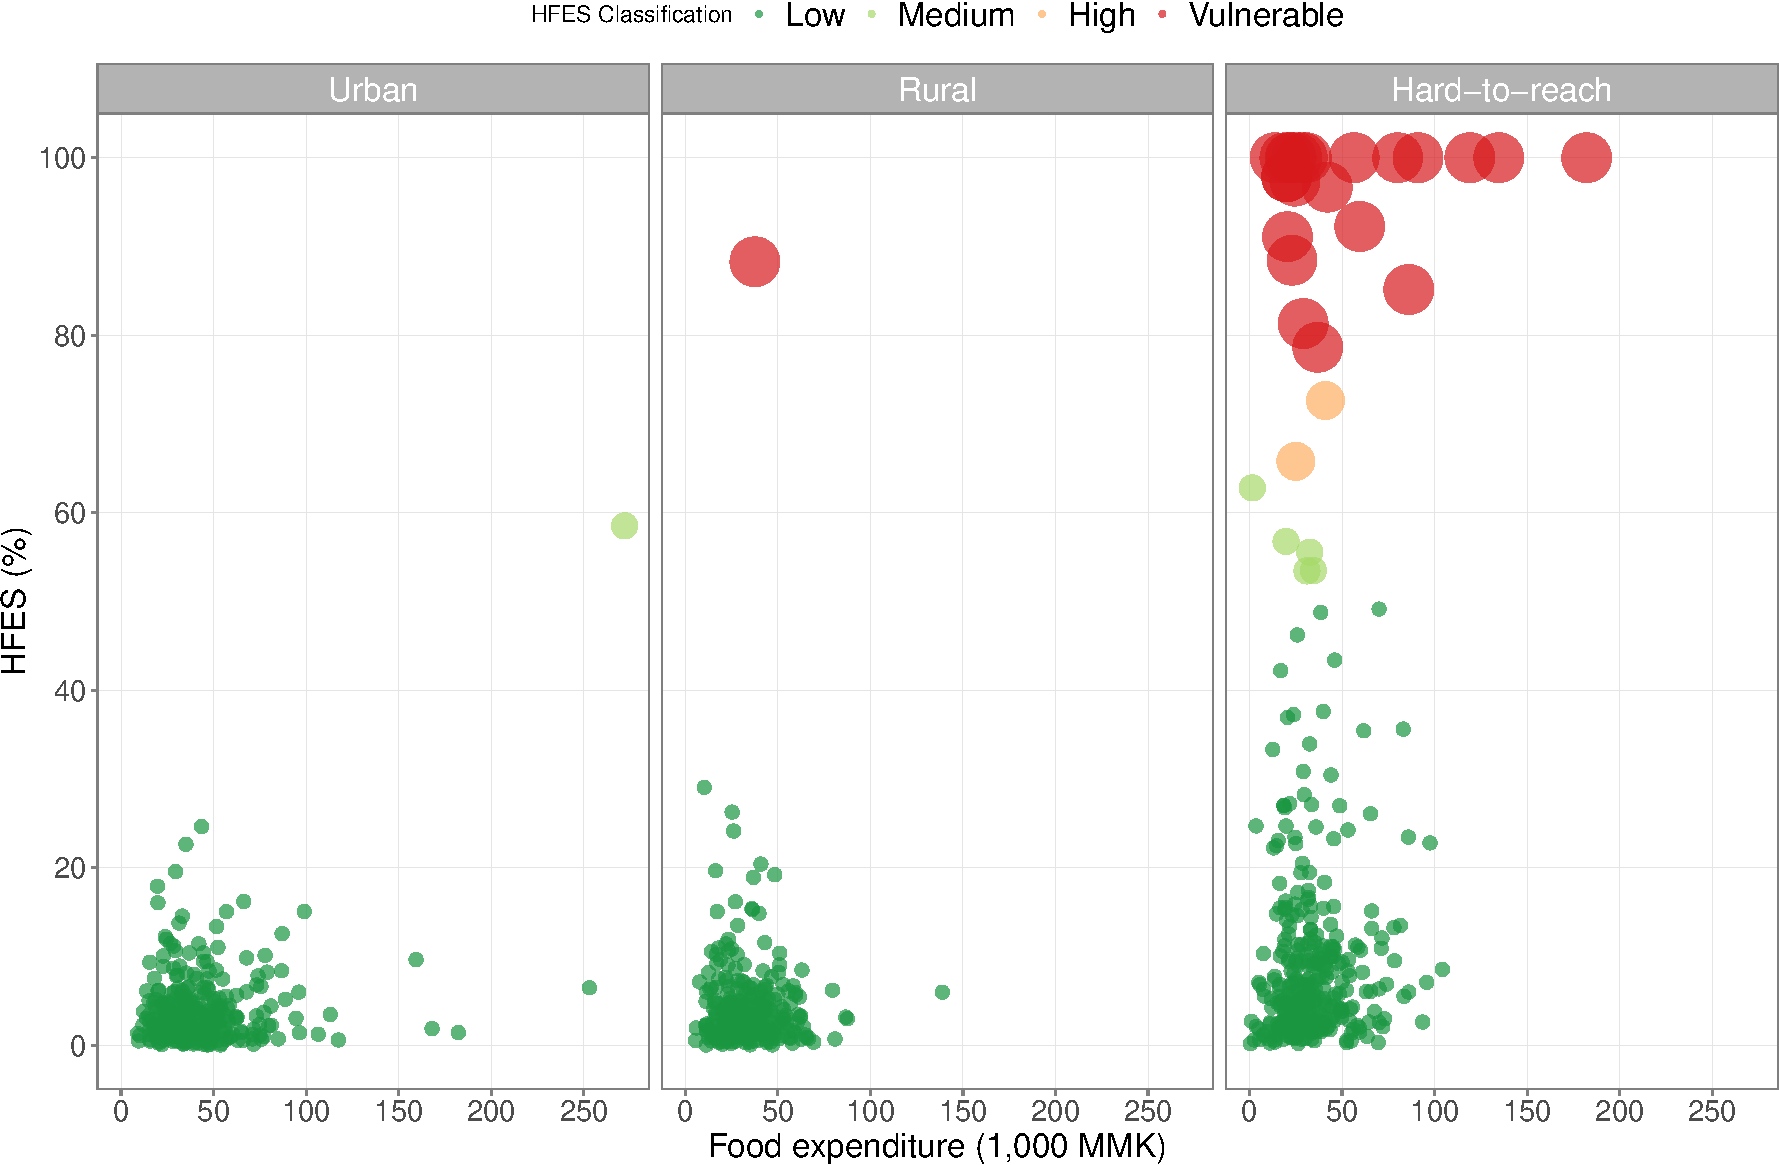
\includegraphics{kayahReport_files/figure-latex/hfesScatterPlot1-1} 

}

\caption{Household food expenditure share by location type}\label{fig:hfesScatterPlot1}
\end{figure}

\begin{figure}[H]

{\centering 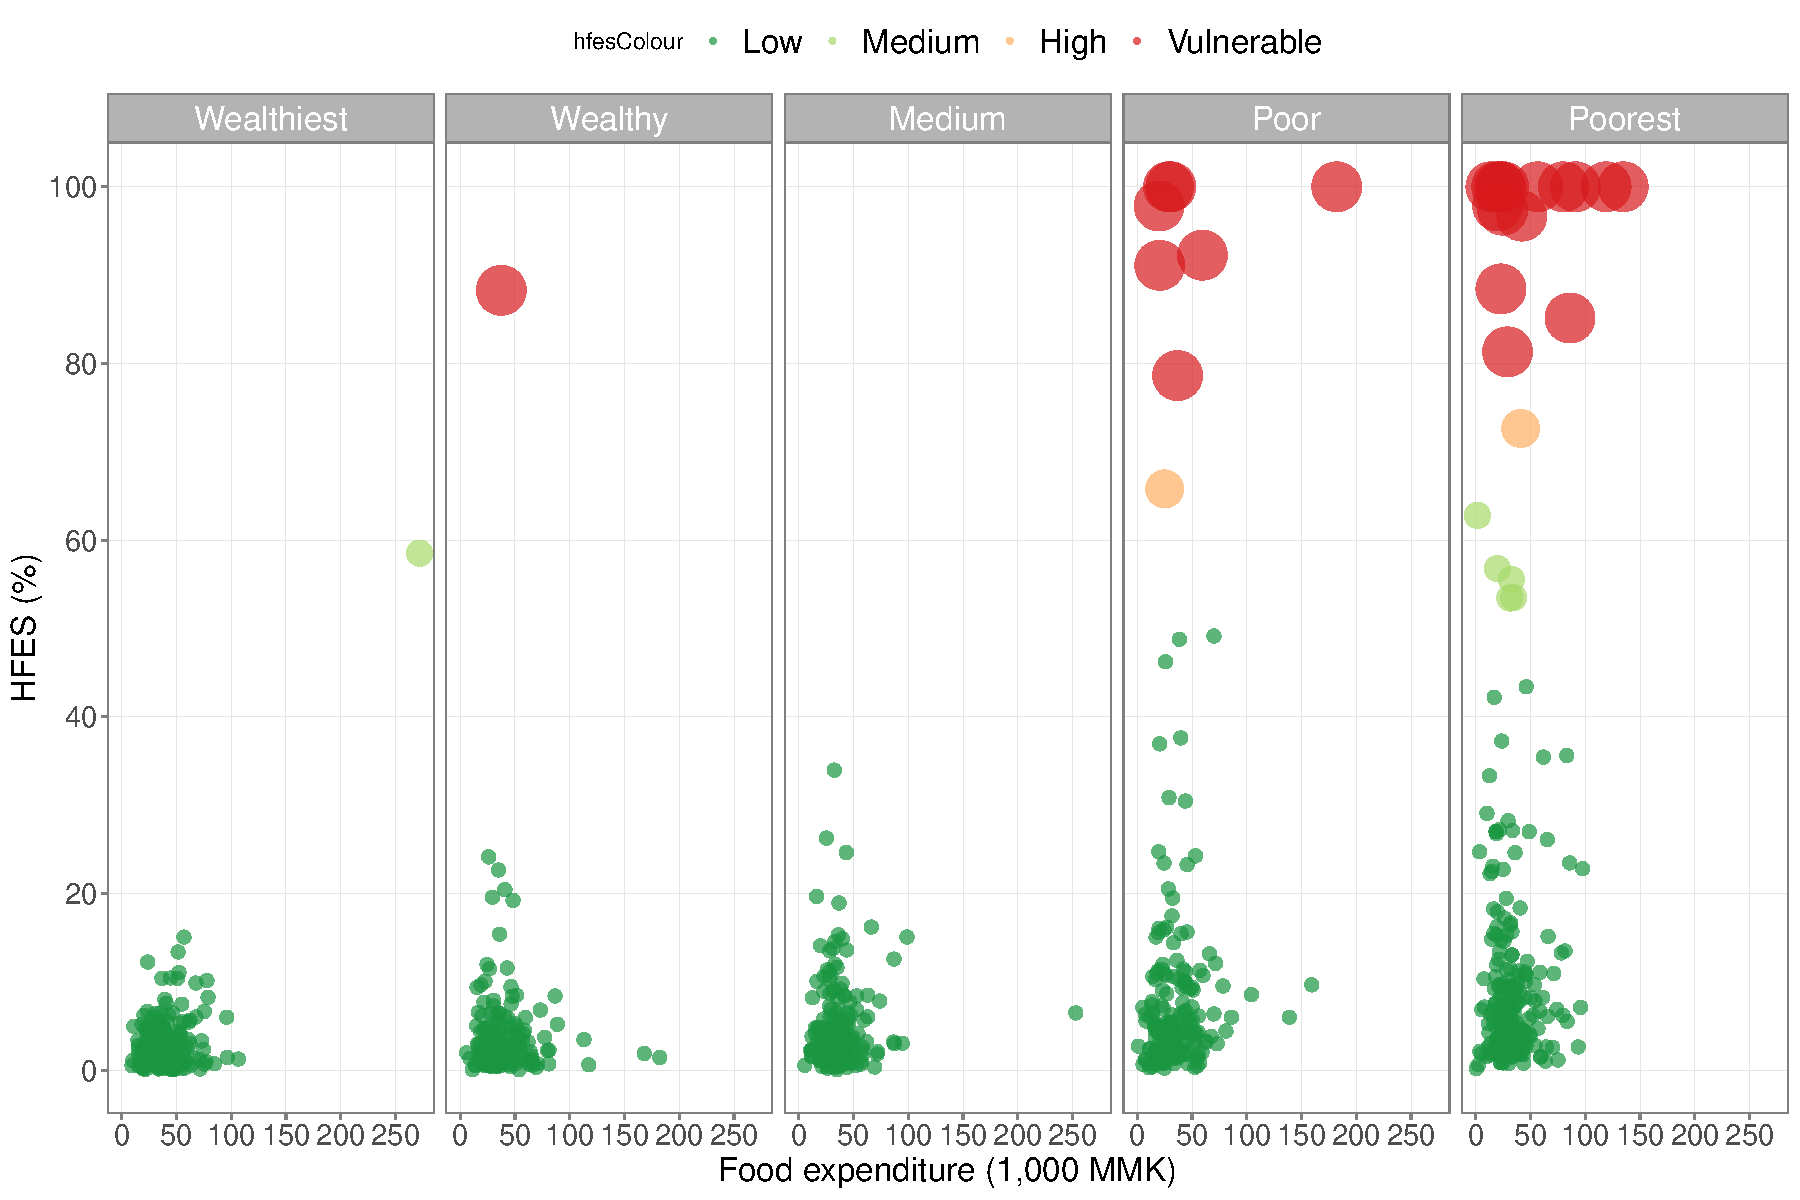
\includegraphics{kayahReport_files/figure-latex/hfesScatterPlot2-1} 

}

\caption{Household food expenditure share by wealth quintiles}\label{fig:hfesScatterPlot2}
\end{figure}

\begin{table}[H]

\caption{\label{tab:hfes2table}Household food expenditure share}
\centering
\fontsize{12}{14}\selectfont
\begin{tabular}[t]{>{\bfseries}l>{\bfseries}l>{\ttfamily}r>{\ttfamily}r>{\ttfamily}r>{\ttfamily}r}
\toprule
\multicolumn{2}{c}{ } & \multicolumn{4}{c}{Food Insecurity by HFES} \\
\cmidrule(l{3pt}r{3pt}){3-6}
 &  & \makecell[c]{Vulnerable\\(\%)} & \makecell[c]{High\\(\%)} & \makecell[c]{Medium\\(\%)} & \makecell[c]{Low\\(\%)}\\
\midrule
\addlinespace[0.3em]
\multicolumn{6}{l}{\textbf{Kayah}}\\
\addlinespace[0.3em]
\multicolumn{6}{l}{\textit{\textbf{Geographic}}}\\
\hspace{1em}\hspace{1em} & Rural & 1.2 & 0.3 & 0.0 & 98.6\\
\cmidrule{2-6}
\hspace{1em}\hspace{1em} & Urban & 0.2 & 0.2 & 0.0 & 99.5\\
\cmidrule{2-6}
\hspace{1em}\hspace{1em} & Hard-to-reach & 1.1 & 1.7 & 1.4 & 95.7\\
\cmidrule{2-6}
\addlinespace[0.3em]
\multicolumn{6}{l}{\textit{\textbf{Wealth}}}\\
\hspace{1em}\hspace{1em} & Wealthiest & 0.0 & 0.0 & 0.0 & 100.0\\
\cmidrule{2-6}
\hspace{1em}\hspace{1em} & Wealthy & 0.0 & 0.0 & 0.0 & 100.0\\
\cmidrule{2-6}
\hspace{1em}\hspace{1em} & Medium & 1.4 & 1.4 & 0.0 & 97.2\\
\cmidrule{2-6}
\hspace{1em}\hspace{1em} & Poor & 1.4 & 0.5 & 0.5 & 97.7\\
\cmidrule{2-6}
\hspace{1em}\hspace{1em} & Poorest & 1.3 & 1.8 & 1.8 & 95.1\\
\bottomrule
\end{tabular}
\end{table}

\begin{figure}[H]

{\centering 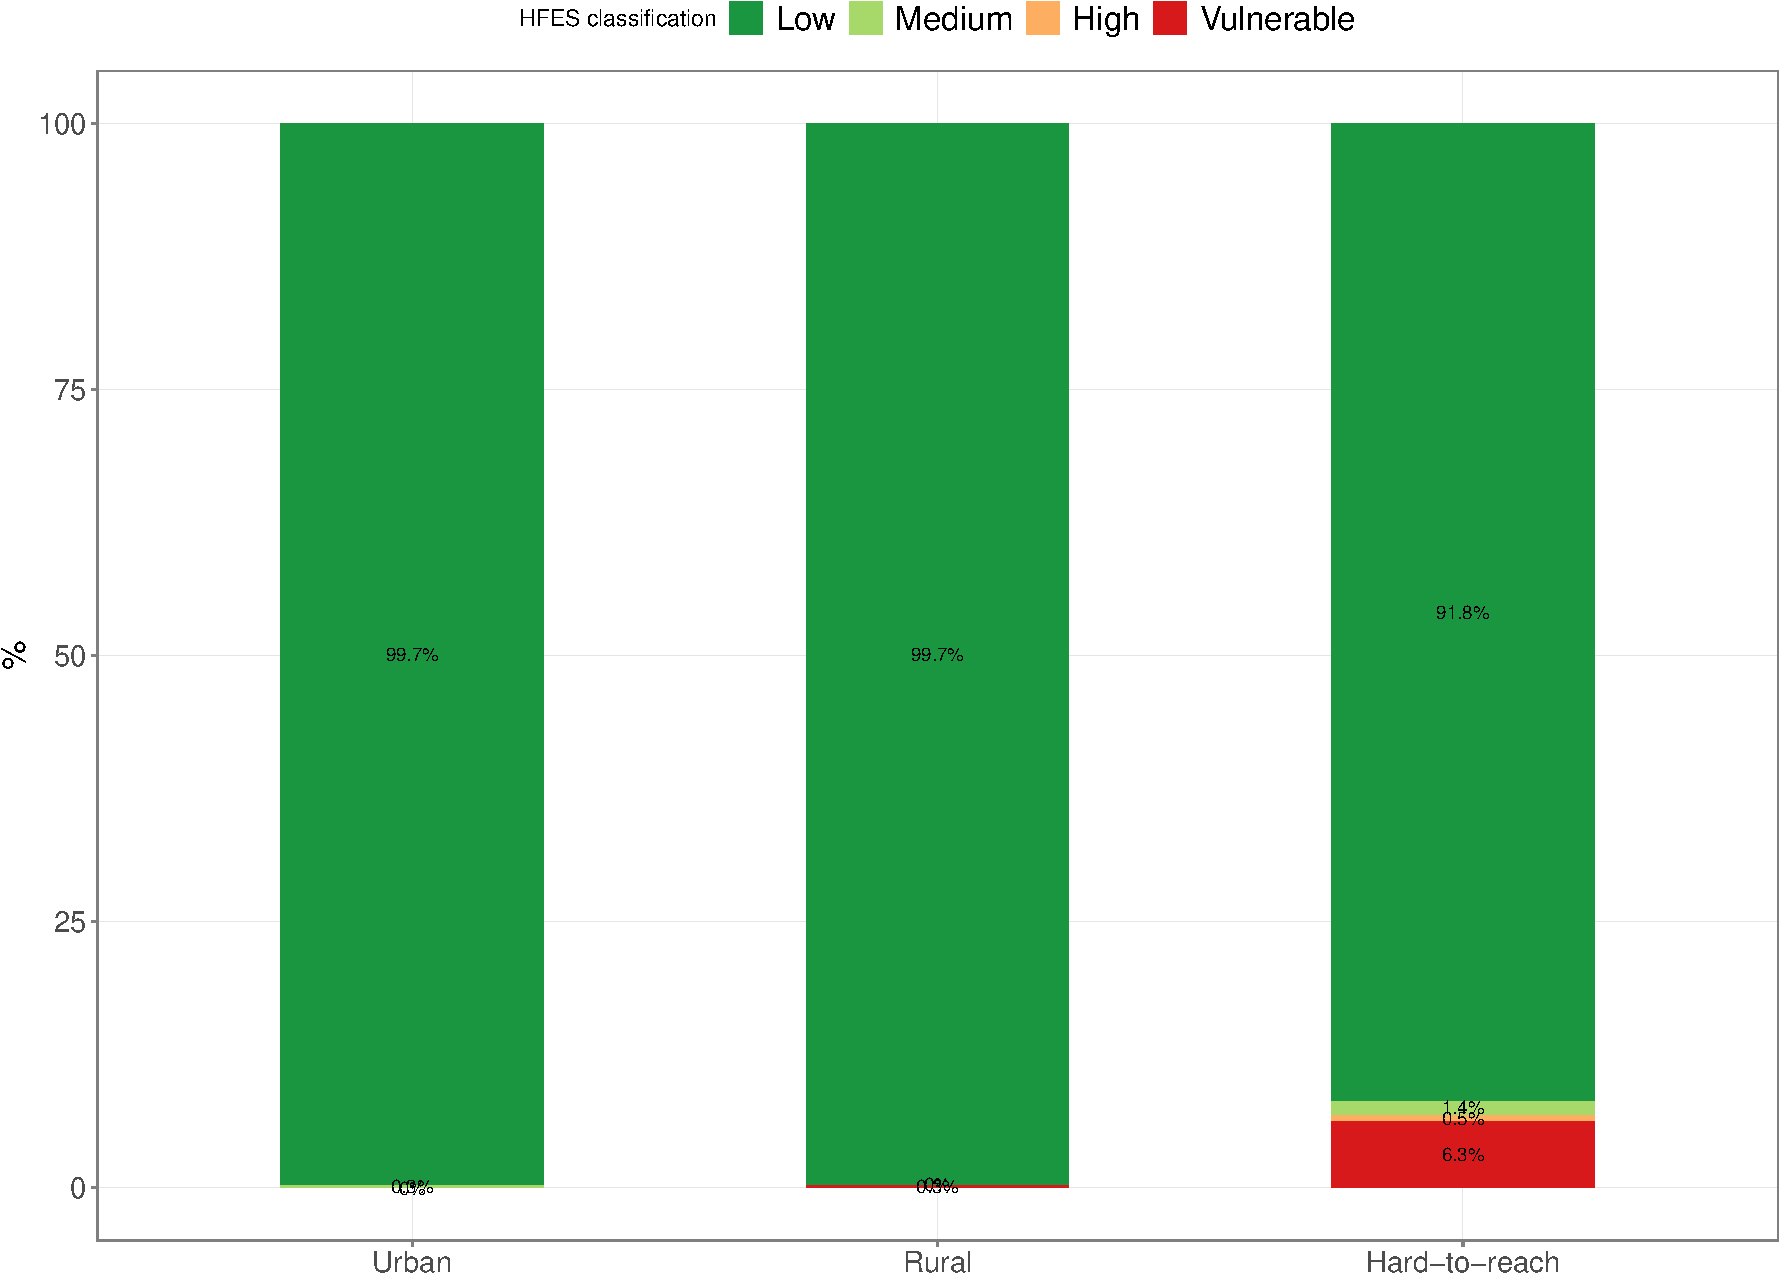
\includegraphics{kayahReport_files/figure-latex/hfes1plot-1} 

}

\caption{Household food expenditure share by location type}\label{fig:hfes1plot}
\end{figure}

\begin{figure}[H]

{\centering 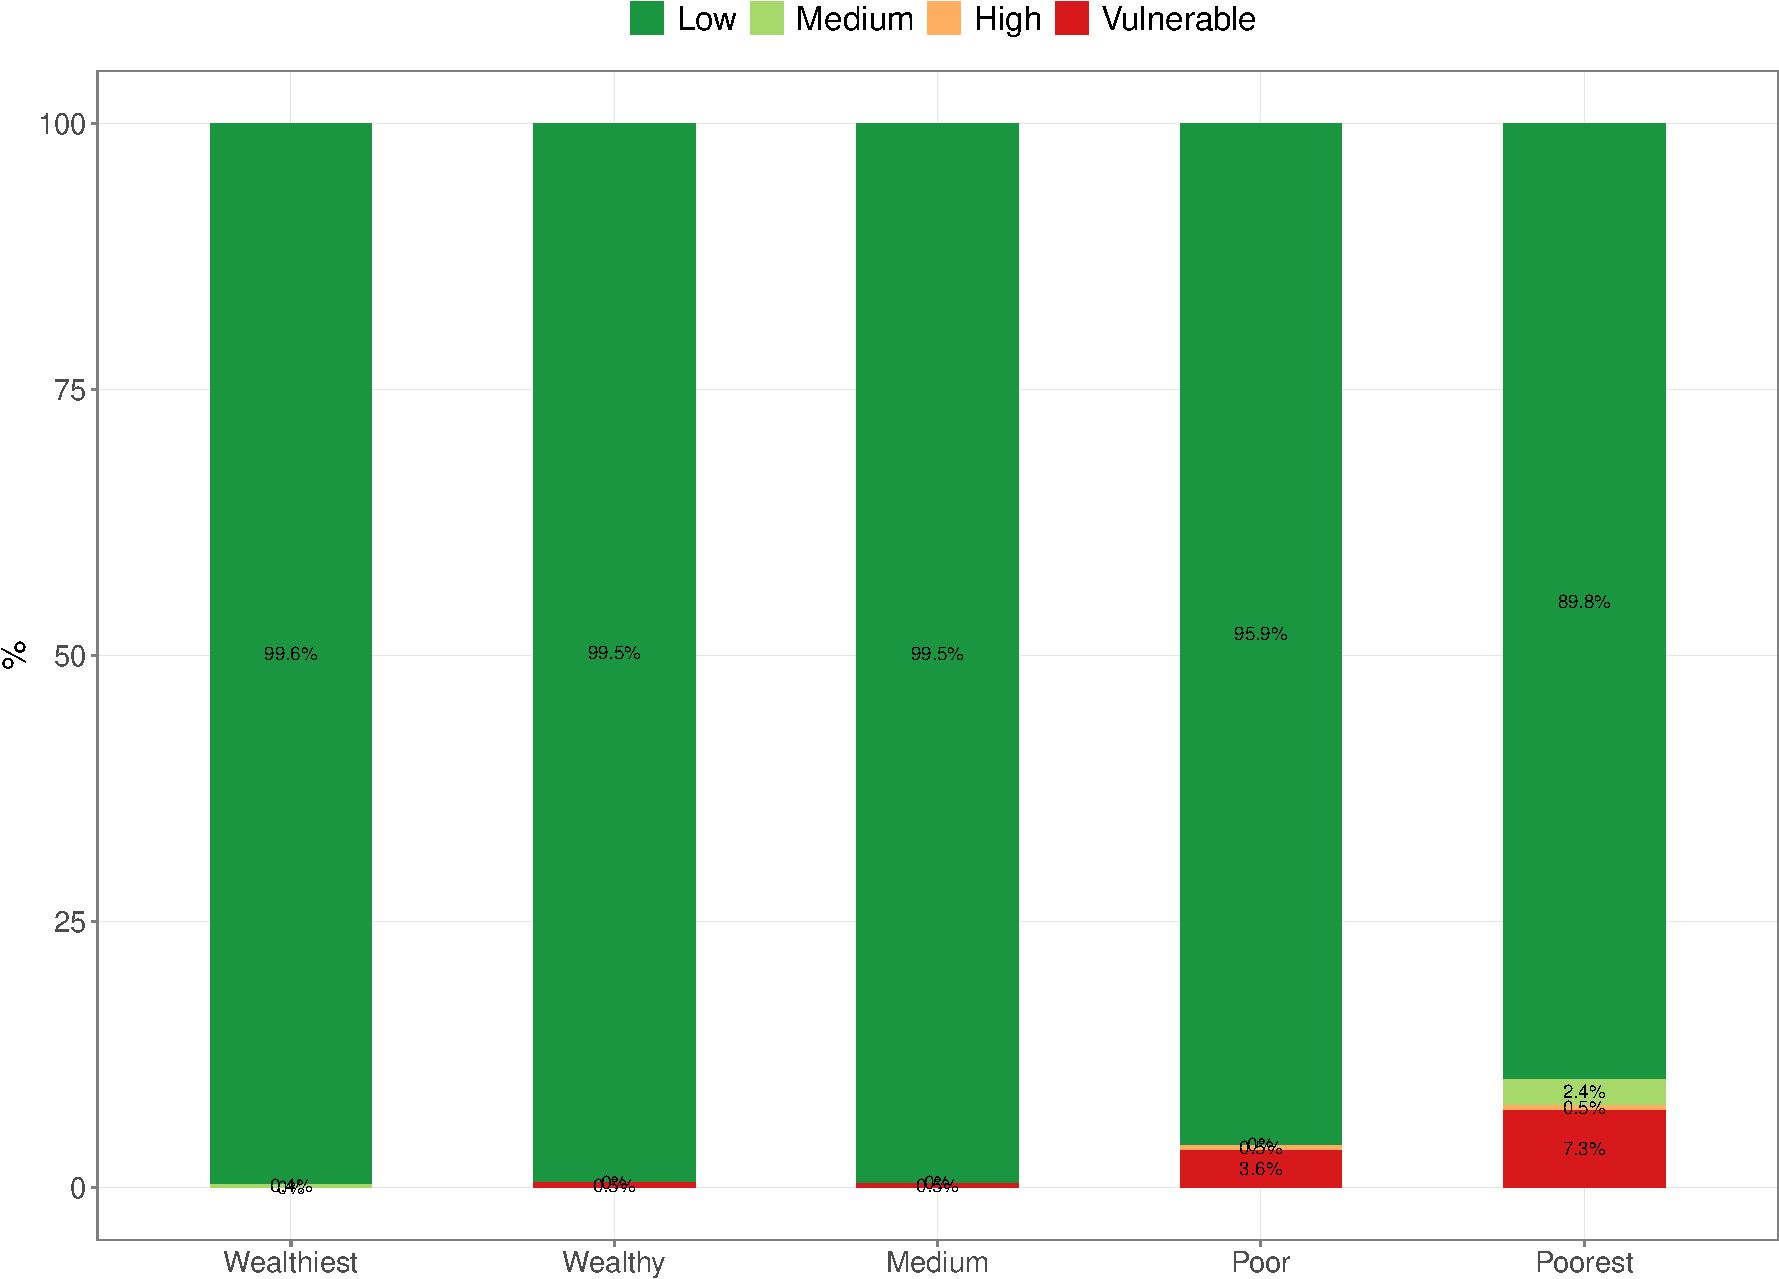
\includegraphics{kayahReport_files/figure-latex/hfes2plot-1} 

}

\caption{Household food expenditure share by wealth quintiles}\label{fig:hfes2plot}
\end{figure}

\hypertarget{wash-results}{%
\subsubsection{Water, sanitation and hygiene}\label{wash-results}}

\hypertarget{water-results}{%
\paragraph{Water services ladder}\label{water-results}}

\begin{landscape}\begin{table}[H]

\caption{\label{tab:wash1table}Water service ladders}
\centering
\fontsize{10}{12}\selectfont
\begin{tabular}[t]{>{\bfseries}l>{\bfseries}l>{\ttfamily}r>{\ttfamily}r>{\ttfamily}r>{\ttfamily}r>{\ttfamily}r>{\ttfamily}r>{\ttfamily}r>{\ttfamily}r>{\ttfamily}r}
\toprule
\multicolumn{2}{c}{\textbf{ }} & \multicolumn{3}{c}{\textbf{Summer Season}} & \multicolumn{3}{c}{\textbf{Rainy Season}} & \multicolumn{3}{c}{\textbf{Winter Season}} \\
\cmidrule(l{3pt}r{3pt}){3-5} \cmidrule(l{3pt}r{3pt}){6-8} \cmidrule(l{3pt}r{3pt}){9-11}
 &  & \makecell[c]{At least\\limited\\(\%)} & \makecell[c]{Unimproved\\(\%)} & \makecell[c]{Surface\\water\\(\%)} & \makecell[c]{At least\\limited\\(\%)} & \makecell[c]{Unimproved\\(\%)} & \makecell[c]{Surface\\water\\(\%)} & \makecell[c]{At least\\limited\\(\%)} & \makecell[c]{Unimproved\\(\%)} & \makecell[c]{Surface\\water\\(\%)}\\
\midrule
\addlinespace[0.3em]
\multicolumn{11}{l}{\textbf{Kayah}}\\
\addlinespace[0.3em]
\multicolumn{11}{l}{\textit{\textbf{Geographic}}}\\
\hspace{1em}\hspace{1em} & Rural & 90.8 & 5.2 & 4.0 & 91.0 & 5.8 & 3.2 & 91.0 & 5.2 & 3.8\\
\cmidrule{2-11}
\hspace{1em}\hspace{1em} & Urban & 95.8 & 3.5 & 0.7 & 96.3 & 3.5 & 0.2 & 96.0 & 3.5 & 0.5\\
\cmidrule{2-11}
\hspace{1em}\hspace{1em} & Hard-to-reach & 57.5 & 17.9 & 24.5 & 65.0 & 15.1 & 19.9 & 59.8 & 16.8 & 23.4\\
\cmidrule{2-11}
\addlinespace[0.3em]
\multicolumn{11}{l}{\textit{\textbf{Wealth}}}\\
\hspace{1em}\hspace{1em} & Wealthiest & 97.6 & 1.9 & 0.5 & 98.6 & 1.4 & 0.0 & 97.1 & 2.4 & 0.5\\
\cmidrule{2-11}
\hspace{1em}\hspace{1em} & Wealthy & 91.3 & 4.3 & 4.3 & 93.5 & 4.3 & 2.2 & 91.8 & 3.9 & 4.3\\
\cmidrule{2-11}
\hspace{1em}\hspace{1em} & Medium & 77.0 & 11.1 & 12.0 & 80.2 & 9.2 & 10.6 & 77.9 & 10.6 & 11.5\\
\cmidrule{2-11}
\hspace{1em}\hspace{1em} & Poor & 71.5 & 14.9 & 13.6 & 76.0 & 13.1 & 10.9 & 72.9 & 14.5 & 12.7\\
\cmidrule{2-11}
\hspace{1em}\hspace{1em} & Poorest & 72.6 & 11.2 & 16.1 & 74.9 & 11.7 & 13.5 & 74.9 & 10.3 & 14.8\\
\bottomrule
\end{tabular}
\end{table}
\end{landscape}

\begin{figure}[H]

{\centering 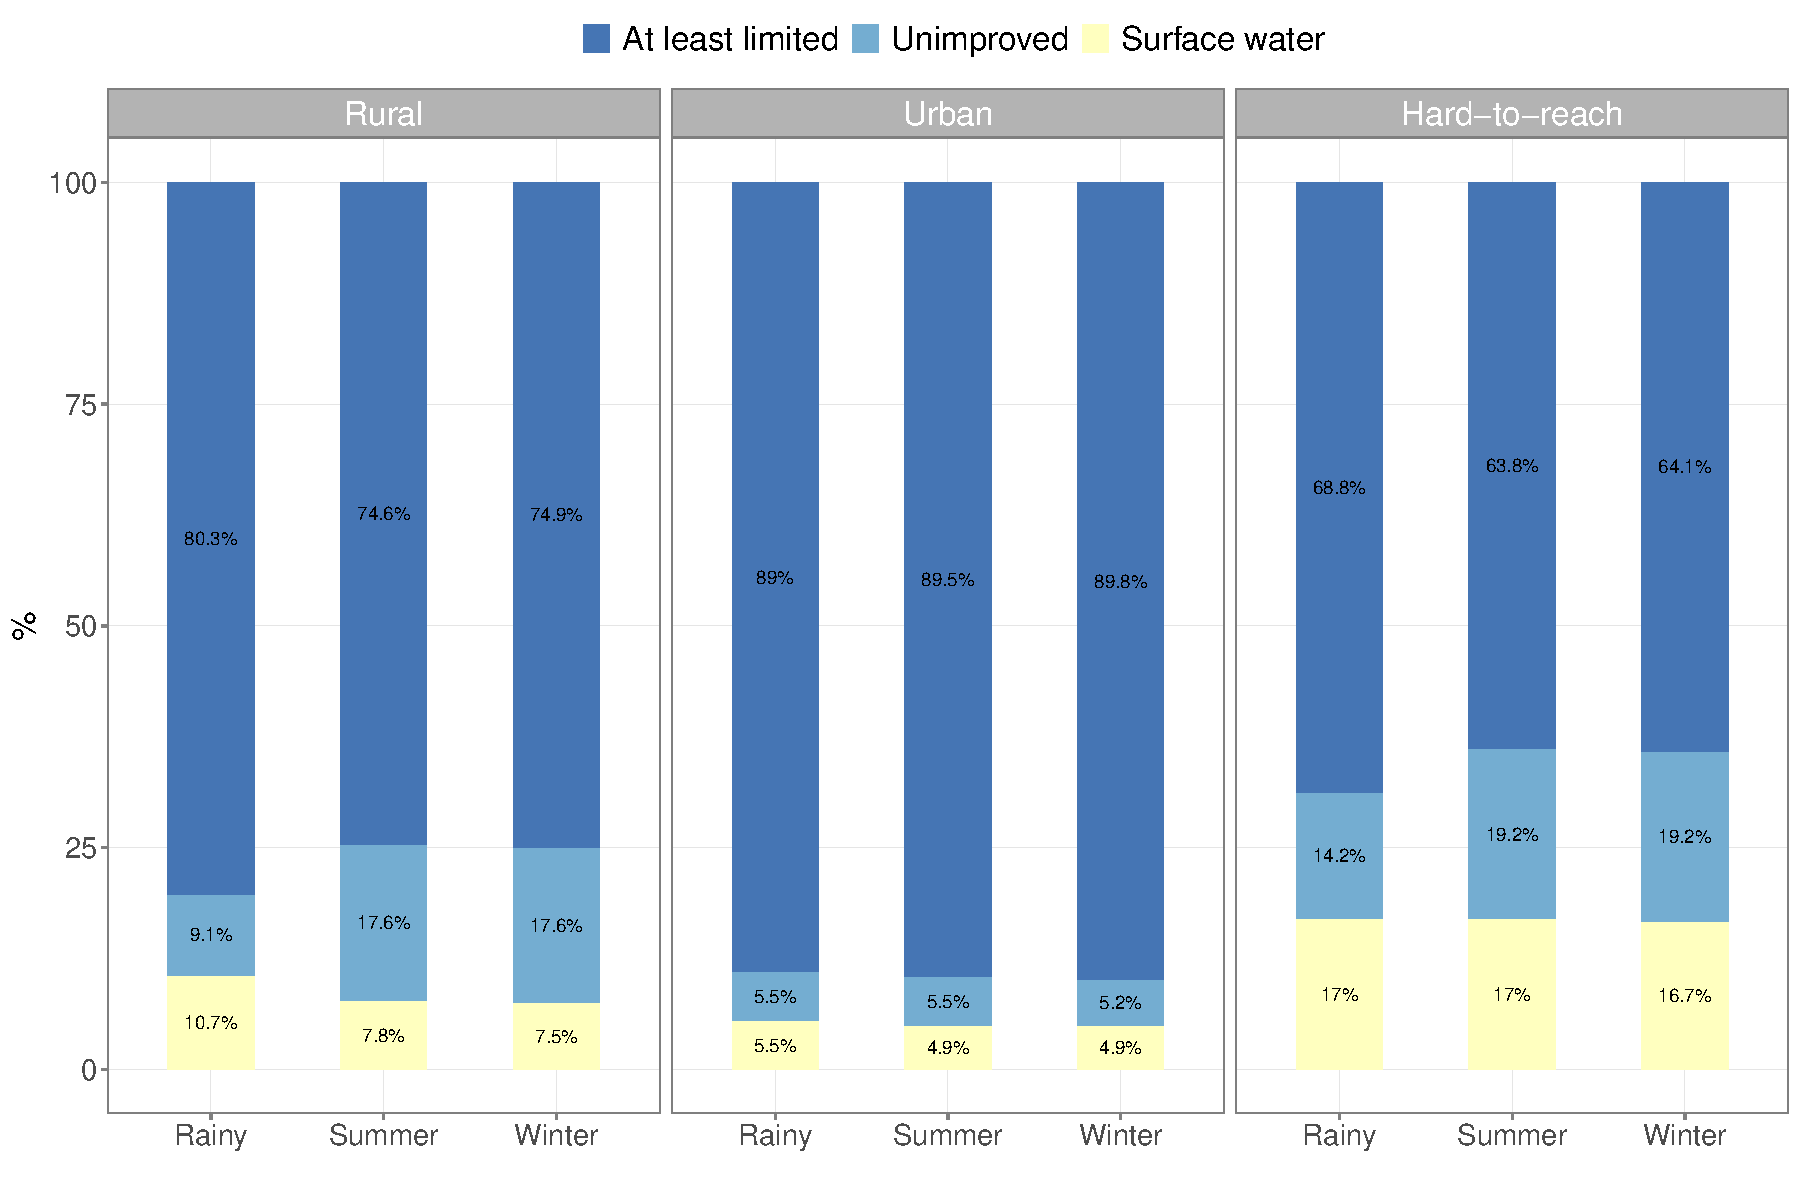
\includegraphics{kayahReport_files/figure-latex/wash1plot-1} 

}

\caption{Water services ladder by location type}\label{fig:wash1plot}
\end{figure}

\begin{figure}[H]

{\centering 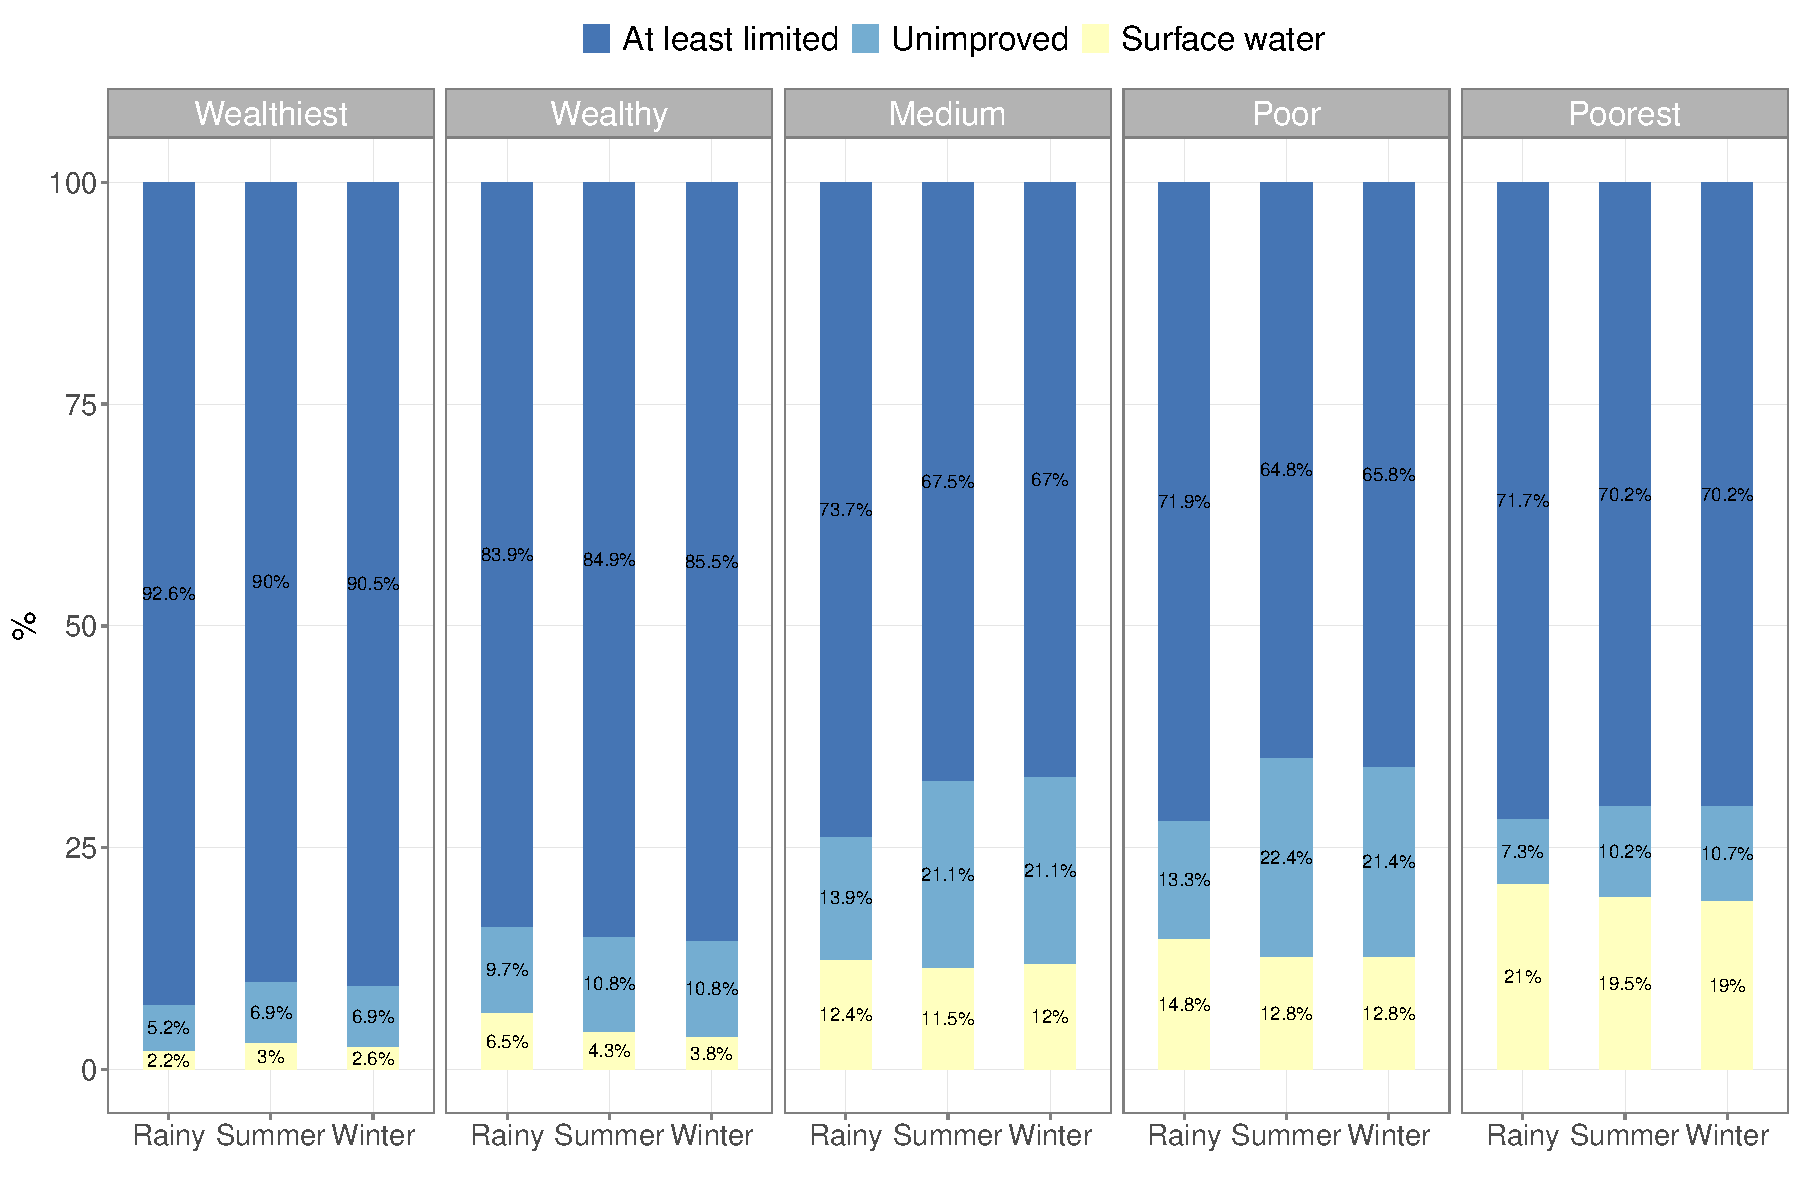
\includegraphics{kayahReport_files/figure-latex/wash2plot-1} 

}

\caption{Water services ladder by wealth quintiles}\label{fig:wash2plot}
\end{figure}

\hypertarget{sanitation-services-ladder}{%
\paragraph{Sanitation services ladder}\label{sanitation-services-ladder}}

\begin{table}[H]

\caption{\label{tab:san1table}Sanitation service ladders}
\centering
\fontsize{12}{14}\selectfont
\begin{tabular}[t]{>{\bfseries}l>{\bfseries}l>{\ttfamily}r>{\ttfamily}r>{\ttfamily}r>{\ttfamily}r}
\toprule
 &  & \makecell[c]{Basic\\(\%)} & \makecell[c]{Limited\\(\%)} & \makecell[c]{Unimproved\\(\%)} & \makecell[c]{Open\\Defecation\\(\%)}\\
\midrule
\addlinespace[0.3em]
\multicolumn{6}{l}{\textbf{Kayah}}\\
\addlinespace[0.3em]
\multicolumn{6}{l}{\textit{\textbf{Geographic}}}\\
\hspace{1em}\hspace{1em} & Rural & 12.4 & 49.1 & 25.4 & 11.6\\
\cmidrule{2-6}
\hspace{1em}\hspace{1em} & Urban & 14.8 & 63.2 & 20.4 & 0.2\\
\cmidrule{2-6}
\hspace{1em}\hspace{1em} & Hard-to-reach & 16.8 & 32.5 & 14.8 & 35.9\\
\cmidrule{2-6}
\addlinespace[0.3em]
\multicolumn{6}{l}{\textit{\textbf{Wealth}}}\\
\hspace{1em}\hspace{1em} & Wealthiest & 14.4 & 77.5 & 7.7 & 0.0\\
\cmidrule{2-6}
\hspace{1em}\hspace{1em} & Wealthy & 14.3 & 63.2 & 19.0 & 2.6\\
\cmidrule{2-6}
\hspace{1em}\hspace{1em} & Medium & 17.5 & 42.4 & 29.0 & 10.1\\
\cmidrule{2-6}
\hspace{1em}\hspace{1em} & Poor & 12.2 & 37.1 & 26.7 & 22.6\\
\cmidrule{2-6}
\hspace{1em}\hspace{1em} & Poorest & 14.3 & 25.1 & 19.3 & 39.9\\
\bottomrule
\end{tabular}
\end{table}

\begin{figure}[H]

{\centering 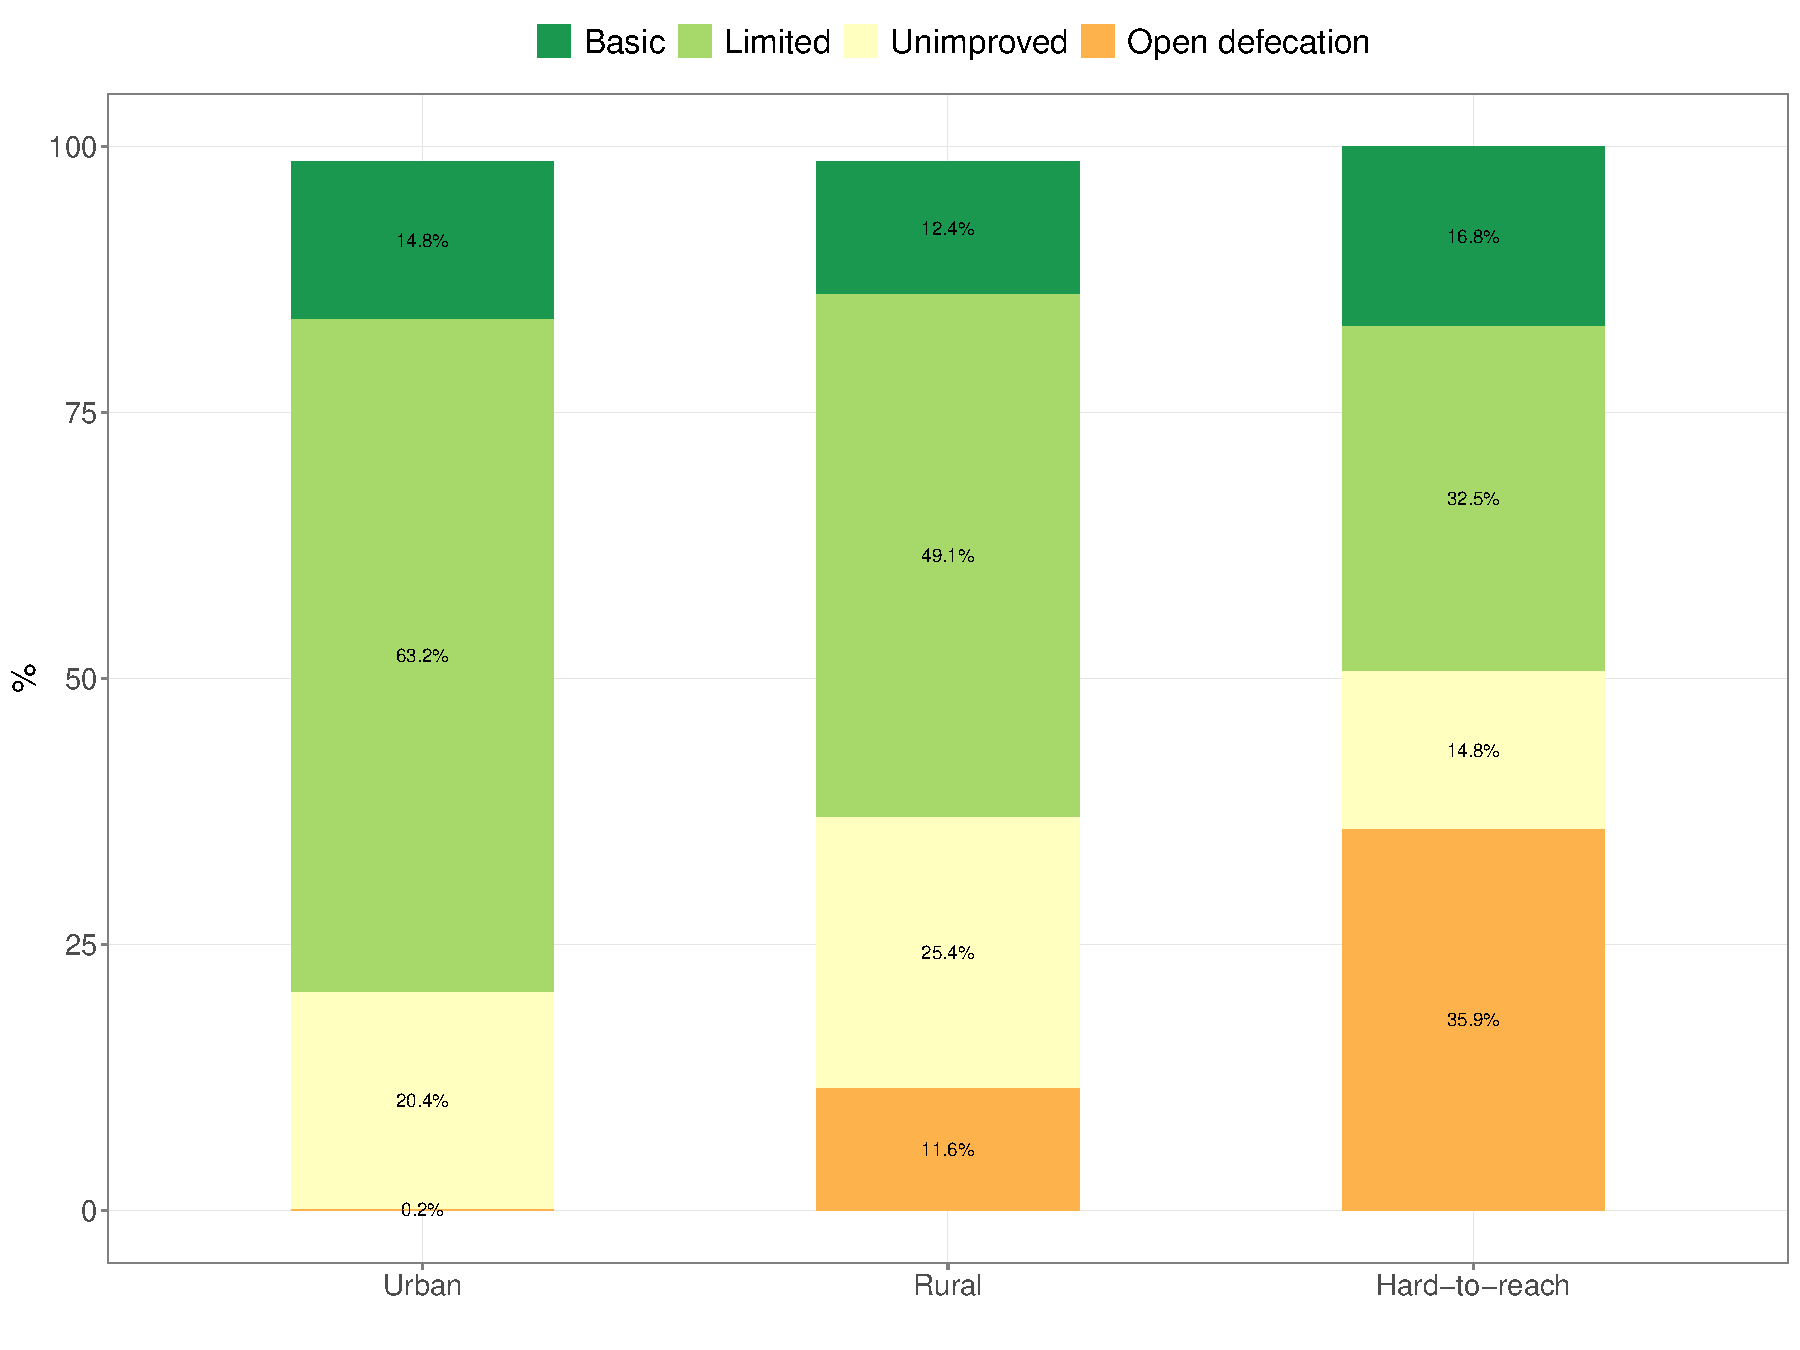
\includegraphics{kayahReport_files/figure-latex/san1plot-1} 

}

\caption{Sanitation services ladder by location type}\label{fig:san1plot}
\end{figure}

\begin{figure}[H]

{\centering 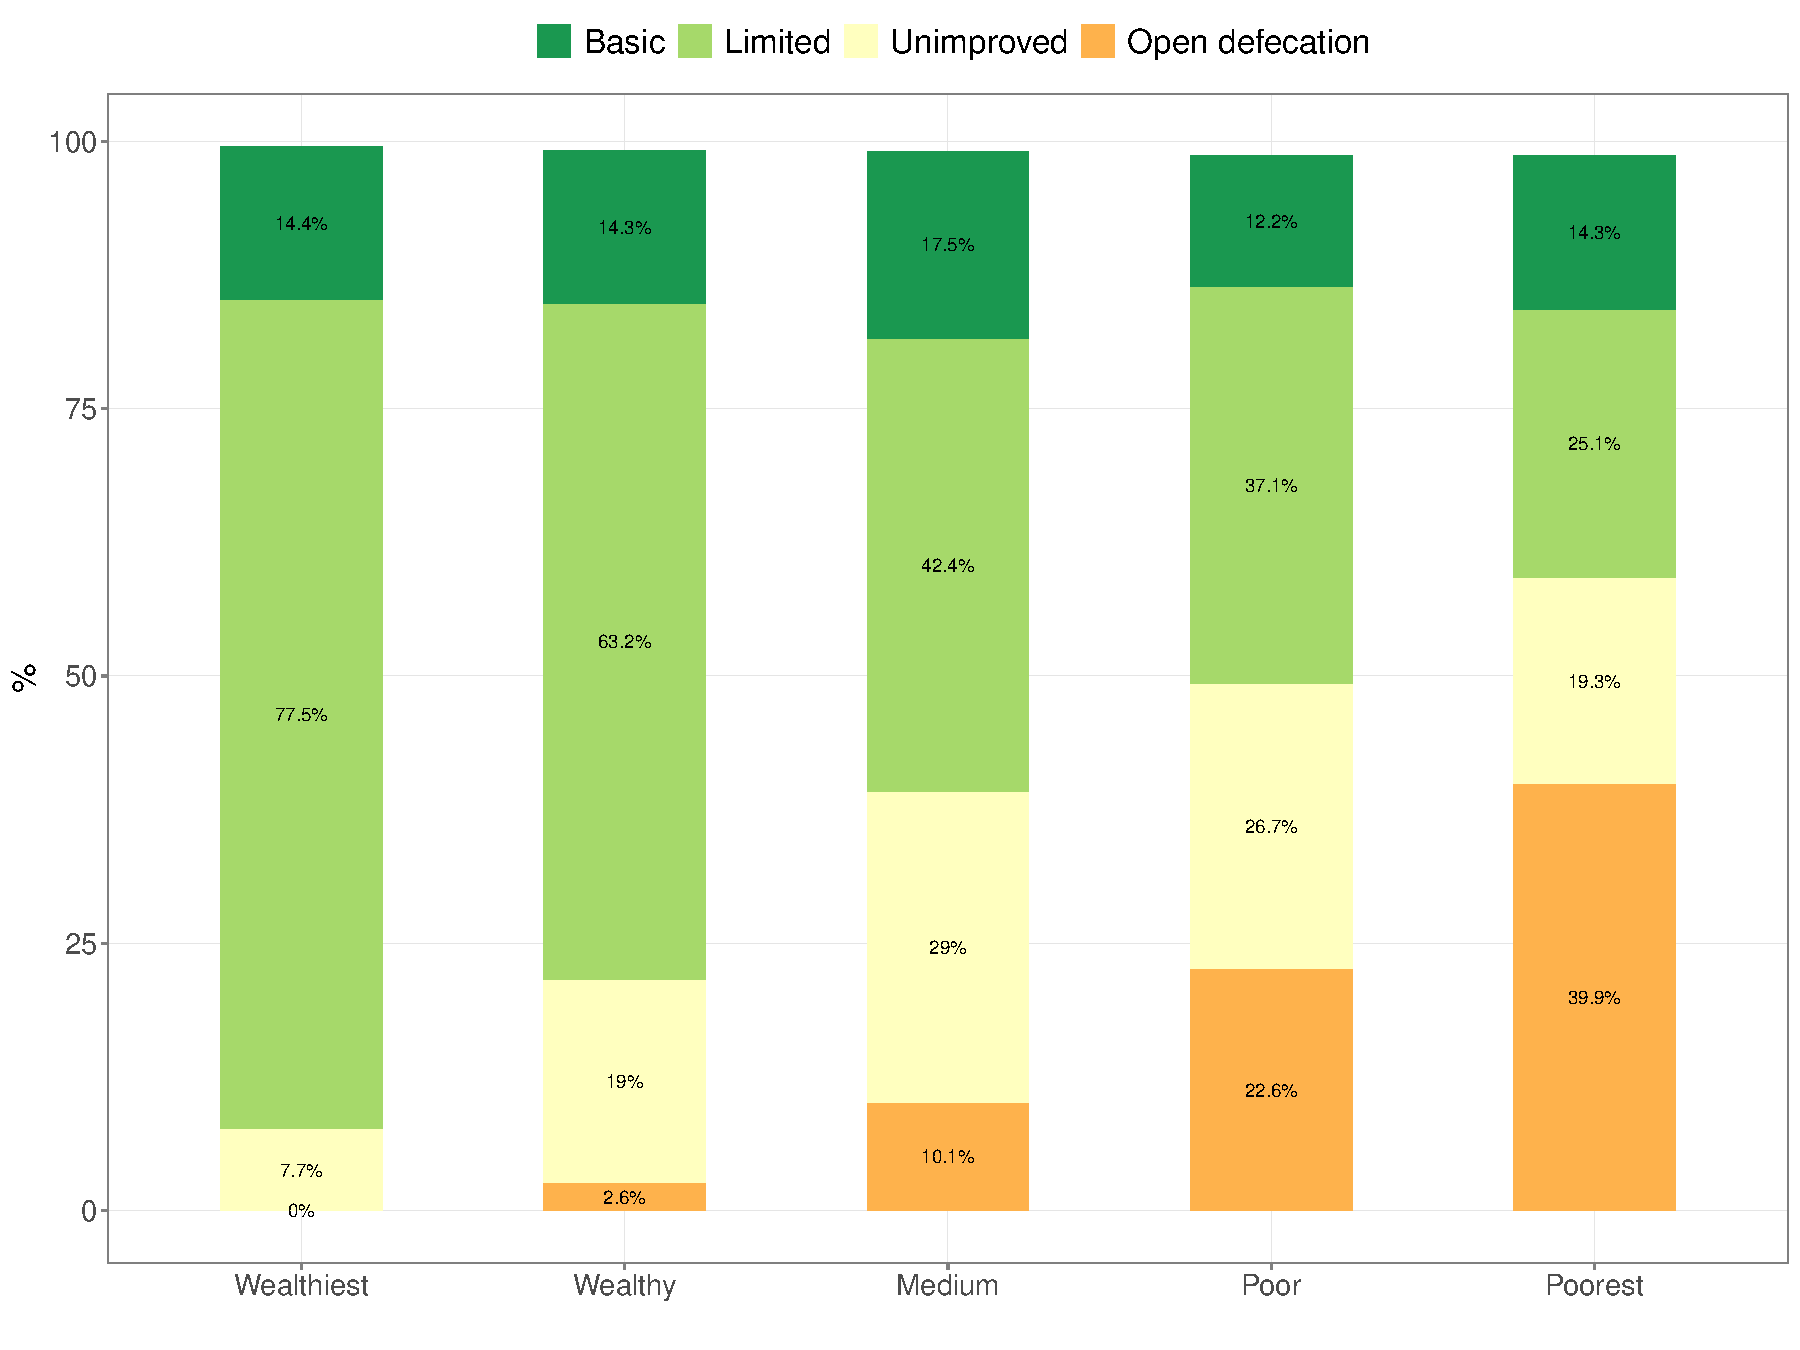
\includegraphics{kayahReport_files/figure-latex/san2plot-1} 

}

\caption{Water services ladder by wealth quintiles}\label{fig:san2plot}
\end{figure}

\hypertarget{handwashing-service-ladders}{%
\paragraph{Handwashing service ladders}\label{handwashing-service-ladders}}

\begin{table}[H]

\caption{\label{tab:handwashing1table}Handwashing service ladders}
\centering
\fontsize{12}{14}\selectfont
\begin{tabular}[t]{>{\bfseries}l>{\bfseries}l>{\ttfamily}r>{\ttfamily}r>{\ttfamily}r}
\toprule
 &  & \makecell[c]{Basic\\(\%)} & \makecell[c]{Limited\\(\%)} & \makecell[c]{No\\Facility\\(\%)}\\
\midrule
\addlinespace[0.3em]
\multicolumn{5}{l}{\textbf{Kayah}}\\
\addlinespace[0.3em]
\multicolumn{5}{l}{\textit{\textbf{Geographic}}}\\
\hspace{1em}\hspace{1em} & Rural & 87.9 & 0.3 & 3.5\\
\cmidrule{2-5}
\hspace{1em}\hspace{1em} & Urban & 93.8 & 0.0 & 2.1\\
\cmidrule{2-5}
\hspace{1em}\hspace{1em} & Hard-to-reach & 45.9 & 2.3 & 6.8\\
\cmidrule{2-5}
\addlinespace[0.3em]
\multicolumn{5}{l}{\textit{\textbf{Wealth}}}\\
\hspace{1em}\hspace{1em} & Wealthiest & 96.2 & 0.0 & 0.5\\
\cmidrule{2-5}
\hspace{1em}\hspace{1em} & Wealthy & 88.7 & 0.0 & 3.5\\
\cmidrule{2-5}
\hspace{1em}\hspace{1em} & Medium & 79.3 & 0.5 & 4.6\\
\cmidrule{2-5}
\hspace{1em}\hspace{1em} & Poor & 67.4 & 0.9 & 6.8\\
\cmidrule{2-5}
\hspace{1em}\hspace{1em} & Poorest & 54.7 & 2.7 & 4.9\\
\bottomrule
\end{tabular}
\end{table}

\begin{figure}[H]

{\centering 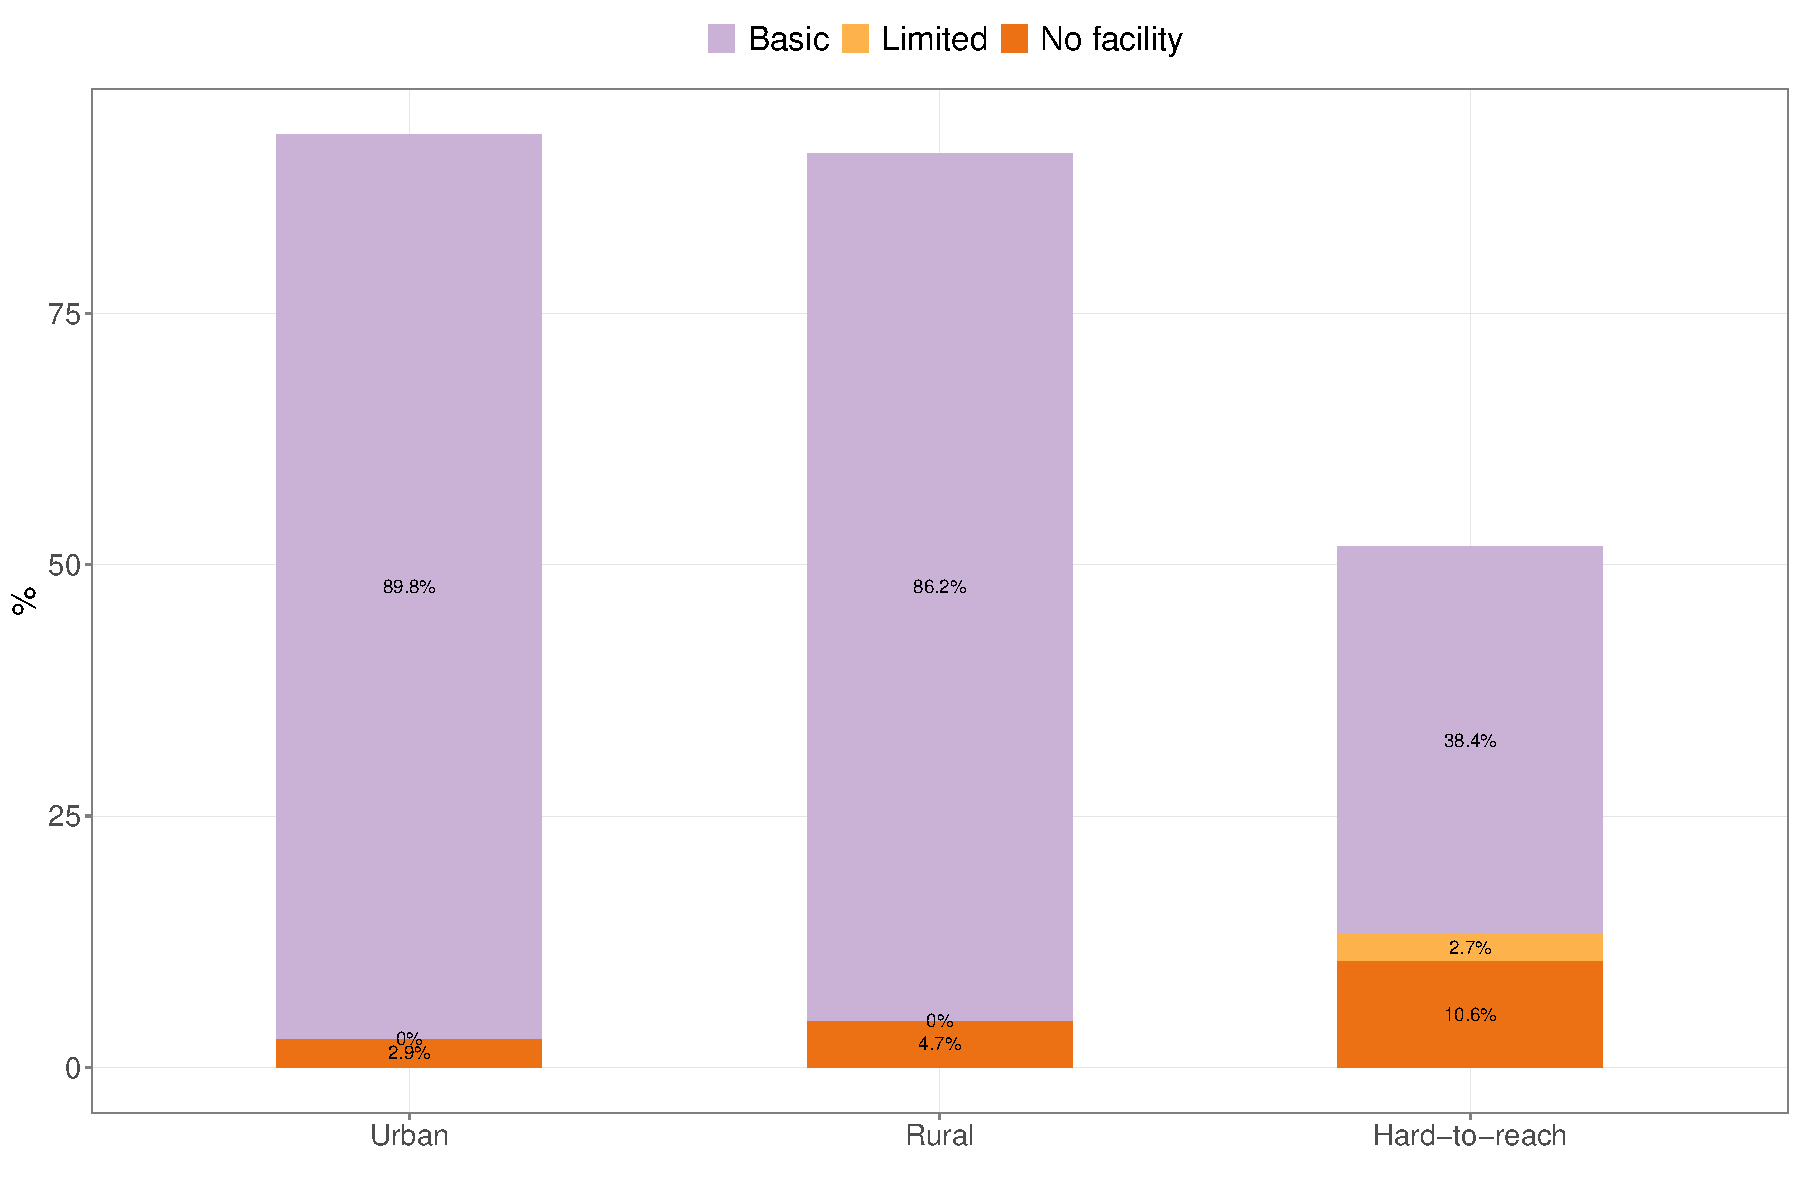
\includegraphics{kayahReport_files/figure-latex/handwashing1plot-1} 

}

\caption{Handwashing services ladder by location type}\label{fig:handwashing1plot}
\end{figure}

\begin{figure}[H]

{\centering 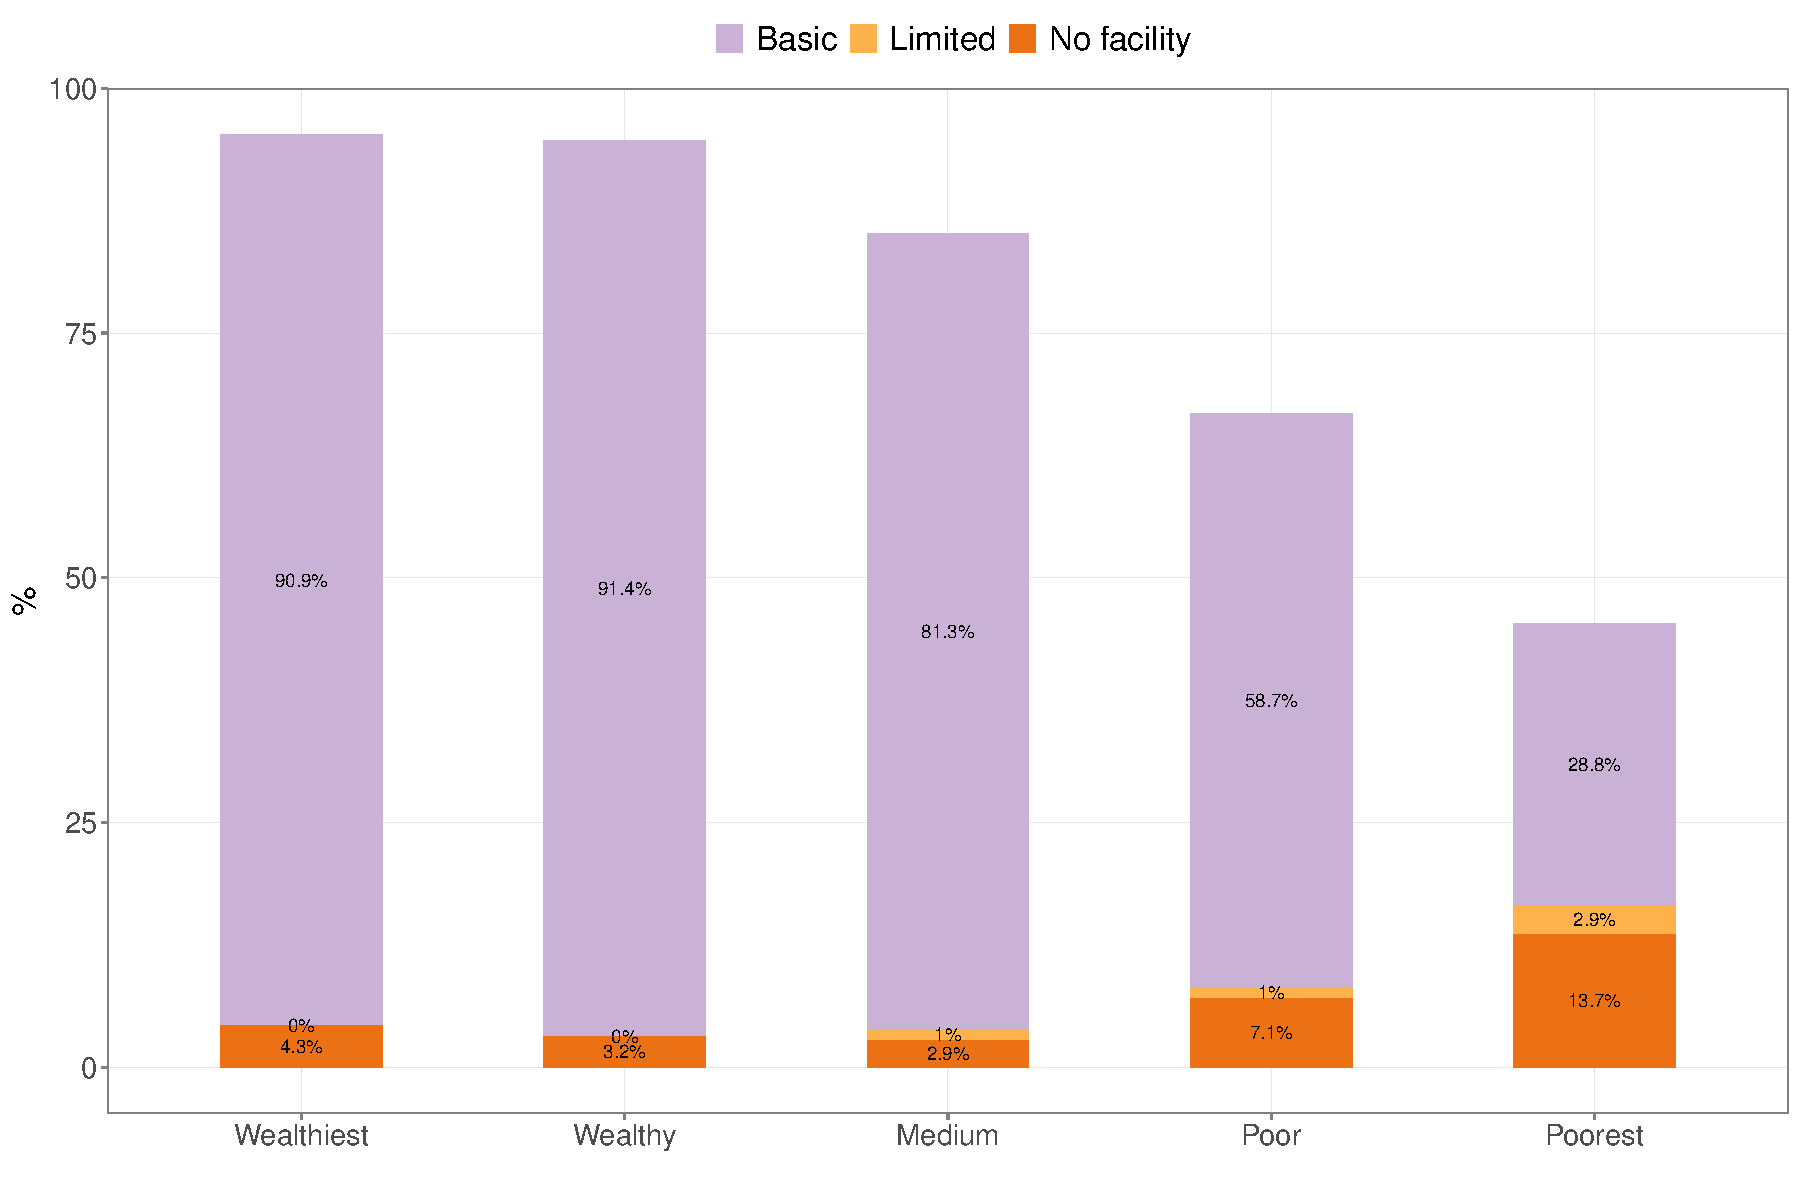
\includegraphics{kayahReport_files/figure-latex/handwashing2plot-1} 

}

\caption{Handwashing services ladder by wealth quintiles}\label{fig:handwashing2plot}
\end{figure}

\hypertarget{chealth-results}{%
\subsubsection{Child health}\label{chealth-results}}

\hypertarget{epi-results}{%
\paragraph{Immunisation coverage}\label{epi-results}}

\begin{landscape}\begin{table}[H]

\caption{\label{tab:epi1table}Immunisation coverage}
\centering
\fontsize{9}{11}\selectfont
\begin{tabular}[t]{>{\bfseries}l>{\bfseries}l>{\ttfamily}r>{\ttfamily}r>{\ttfamily}r>{\ttfamily}r>{\ttfamily}r>{\ttfamily}r}
\toprule
 &  & \makecell[c]{Ever\\vaccinated\\(\%)} & \makecell[c]{Vaccination\\card\\retention\\rate\\(\%)} & \makecell[c]{Immunisation\\access\\(\%)} & \makecell[c]{Immunisation\\utilisation\\(\%)} & \makecell[c]{Full\\immunisation\\coverage\\(\%)} & \makecell[c]{Hepatitis B\\immunisation\\given\\within\\first\\24\\hours\\(\%)}\\
\midrule
\addlinespace[0.3em]
\multicolumn{8}{l}{\textbf{Kayah}}\\
\addlinespace[0.3em]
\multicolumn{8}{l}{\textit{\textbf{Geographic}}}\\
\hspace{1em}\hspace{1em} & Rural & 100.0 & 80.4 & 93.2 & 72.8 & 24.3 & 40.7\\
\cmidrule{2-8}
\hspace{1em}\hspace{1em} & Urban & 98.3 & 82.2 & 92.6 & 76.0 & 25.6 & 55.5\\
\cmidrule{2-8}
\hspace{1em}\hspace{1em} & Hard-to-reach & 85.5 & 75.4 & 81.6 & 50.0 & 19.7 & 25.0\\
\cmidrule{2-8}
\addlinespace[0.3em]
\multicolumn{8}{l}{\textit{\textbf{Wealth}}}\\
\hspace{1em}\hspace{1em} & Wealthiest & 100.0 & 90.7 & 94.5 & 83.6 & 21.8 & 57.5\\
\cmidrule{2-8}
\hspace{1em}\hspace{1em} & Wealthy & 100.0 & 76.1 & 94.4 & 67.6 & 26.8 & 51.9\\
\cmidrule{2-8}
\hspace{1em}\hspace{1em} & Medium & 96.9 & 85.7 & 93.8 & 78.5 & 20.0 & 41.0\\
\cmidrule{2-8}
\hspace{1em}\hspace{1em} & Poor & 94.2 & 81.6 & 81.1 & 62.3 & 30.2 & 36.4\\
\cmidrule{2-8}
\hspace{1em}\hspace{1em} & Poorest & 86.3 & 63.6 & 84.3 & 47.1 & 19.6 & 18.7\\
\bottomrule
\end{tabular}
\end{table}
\end{landscape}

\begin{figure}[H]

{\centering 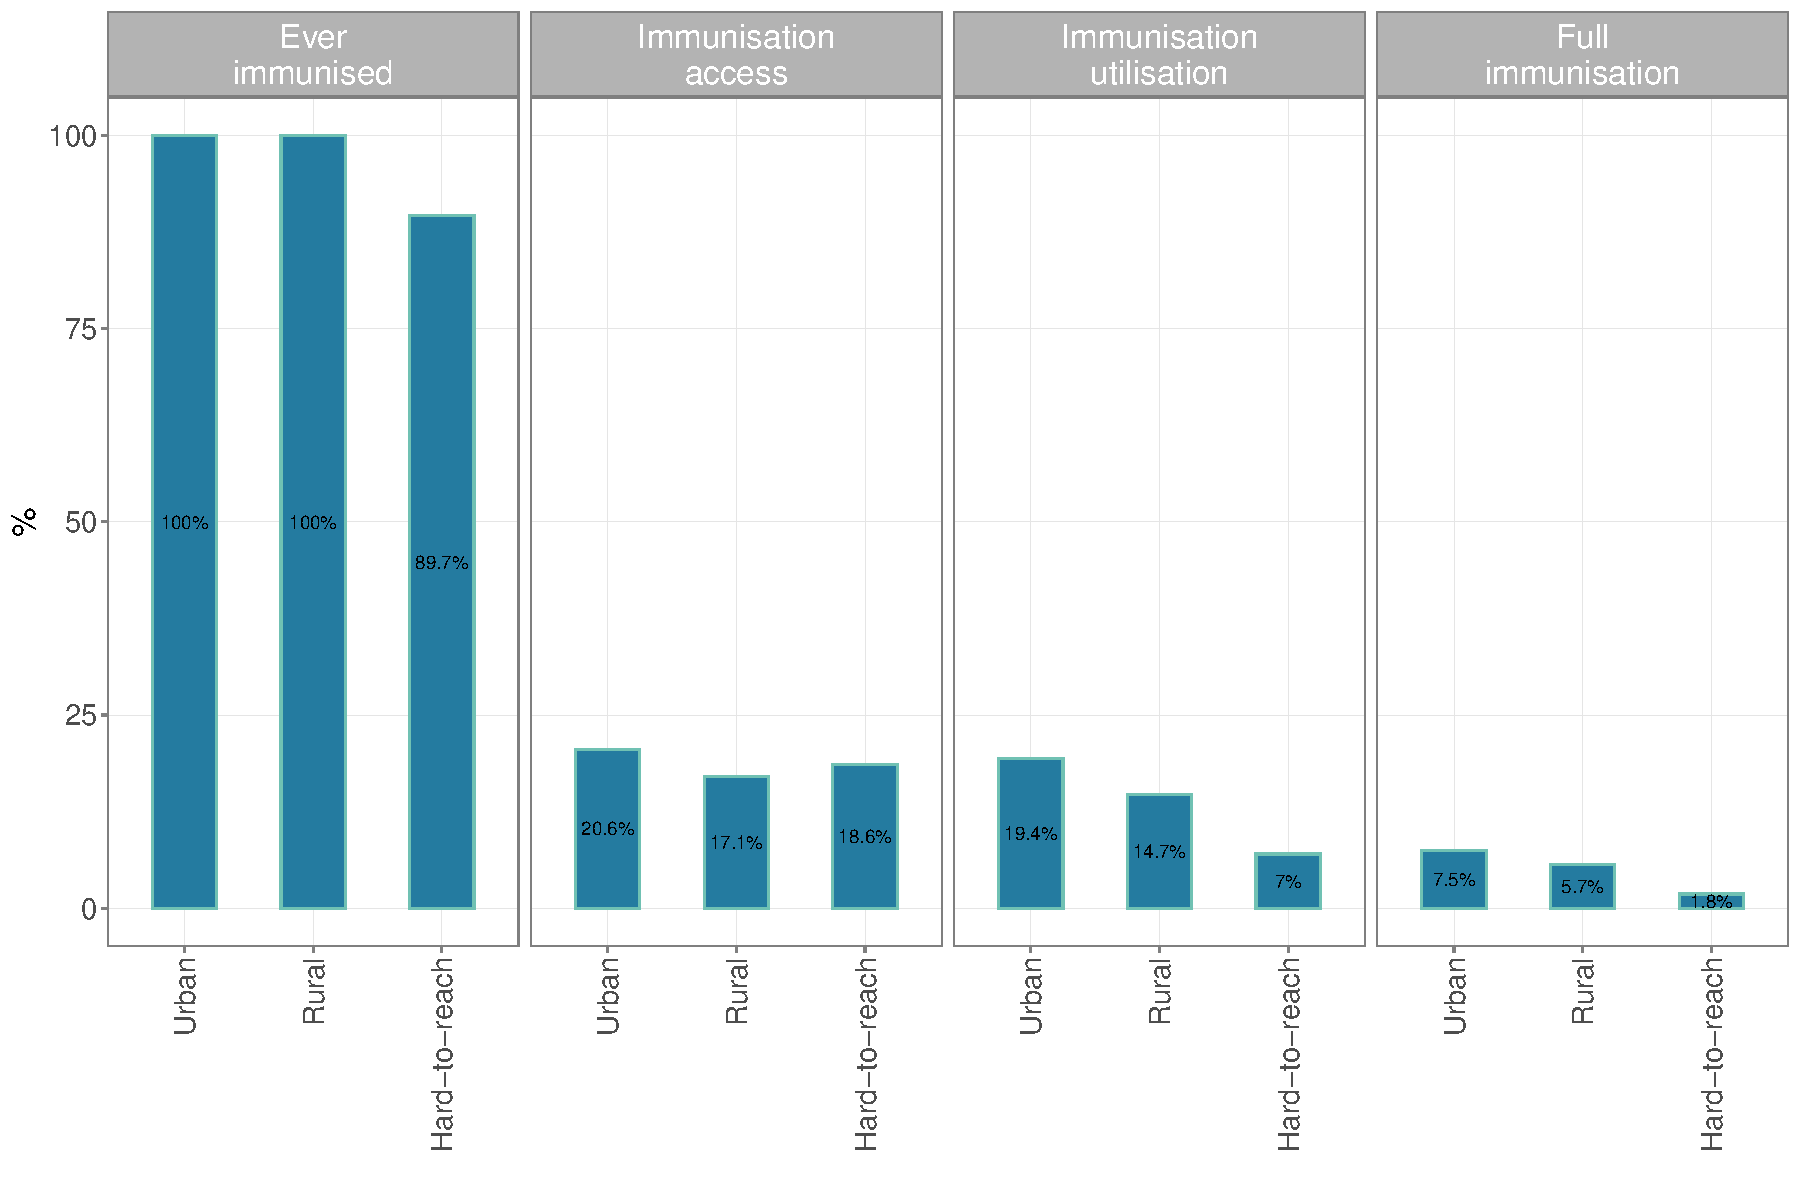
\includegraphics{kayahReport_files/figure-latex/epi1plot-1} 

}

\caption{Immunisation coverage by location type}\label{fig:epi1plot}
\end{figure}

\begin{figure}[H]

{\centering 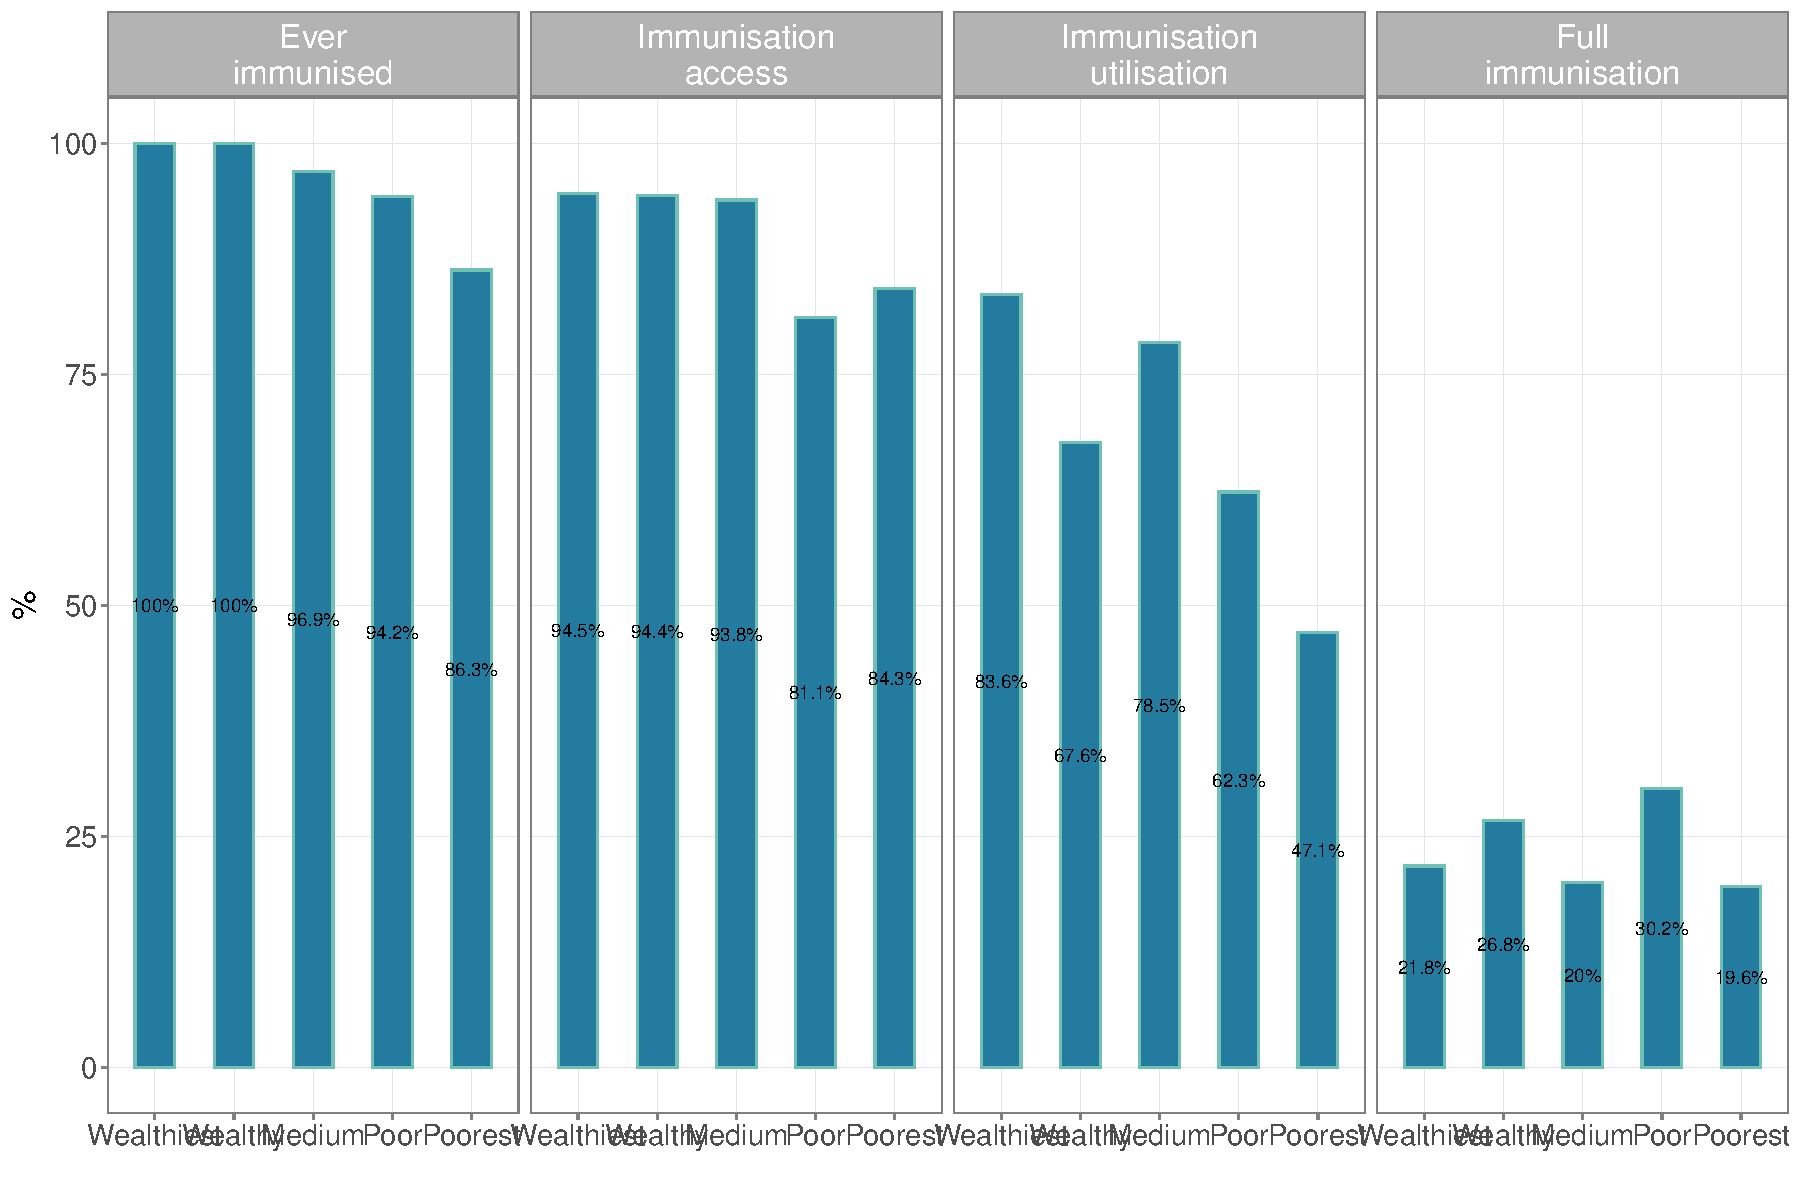
\includegraphics{kayahReport_files/figure-latex/epi2plot-1} 

}

\caption{Immunisation coverage by wealth quintiles}\label{fig:epi2plot}
\end{figure}

\begin{landscape}\begin{table}[H]

\caption{\label{tab:epi2table}Immunisation coverage per vaccine type}
\centering
\fontsize{9}{11}\selectfont
\begin{tabular}[t]{>{\bfseries}l>{\bfseries}l>{\ttfamily}r>{\ttfamily}r>{\ttfamily}r>{\ttfamily}r>{\ttfamily}r>{\ttfamily}r>{\ttfamily}r>{\ttfamily}r>{\ttfamily}r>{\ttfamily}r>{\ttfamily}r>{\ttfamily}r>{\ttfamily}r}
\toprule
 &  & \makecell[c]{BCG\\(\%)} & \makecell[c]{Hepatitis B\\(\%)} & \makecell[c]{Penta 1\\(\%)} & \makecell[c]{Penta 2\\(\%)} & \makecell[c]{Penta 3\\(\%)} & \makecell[c]{OPV 1\\(\%)} & \makecell[c]{OPV 2\\(\%)} & \makecell[c]{OPV 3\\(\%)} & \makecell[c]{IPV\\(\%)} & \makecell[c]{Measles 1\\(\%)} & \makecell[c]{Measles 2\\(\%)} & \makecell[c]{Rubella\\(\%)} & \makecell[c]{Pneumococcal\\(\%)}\\
\midrule
\addlinespace[0.3em]
\multicolumn{15}{l}{\textbf{Kayah}}\\
\addlinespace[0.3em]
\multicolumn{15}{l}{\textit{\textbf{Geographic}}}\\
\hspace{1em}\hspace{1em} & Rural & 21.1 & 13.4 & 17.8 & 17.4 & 16.5 & 17.6 & 17.6 & 17.0 & 14.5 & 17.0 & 11.5 & 13.0 & 10.6\\
\cmidrule{2-15}
\hspace{1em}\hspace{1em} & Urban & 21.5 & 14.8 & 18.7 & 18.7 & 17.7 & 18.5 & 17.9 & 17.3 & 16.5 & 16.5 & 8.5 & 11.3 & 10.6\\
\cmidrule{2-15}
\hspace{1em}\hspace{1em} & Hard-to-reach & 15.2 & 11.2 & 11.5 & 10.5 & 9.3 & 11.5 & 10.3 & 9.0 & 10.0 & 8.8 & 6.6 & 7.3 & 6.6\\
\cmidrule{2-15}
\addlinespace[0.3em]
\multicolumn{15}{l}{\textit{\textbf{Wealth}}}\\
\hspace{1em}\hspace{1em} & Wealthiest & 19.8 & 14.5 & 18.7 & 18.3 & 17.6 & 18.7 & 17.9 & 17.2 & 17.2 & 16.0 & 7.6 & 9.5 & 8.8\\
\cmidrule{2-15}
\hspace{1em}\hspace{1em} & Wealthy & 23.0 & 15.1 & 18.2 & 18.2 & 16.5 & 17.9 & 17.5 & 16.8 & 16.5 & 16.5 & 10.0 & 11.7 & 10.7\\
\cmidrule{2-15}
\hspace{1em}\hspace{1em} & Medium & 21.2 & 14.9 & 18.8 & 18.8 & 17.7 & 18.8 & 18.4 & 17.0 & 14.9 & 17.4 & 9.4 & 10.8 & 10.1\\
\cmidrule{2-15}
\hspace{1em}\hspace{1em} & Poor & 16.7 & 12.0 & 15.1 & 14.0 & 12.8 & 14.7 & 13.2 & 12.8 & 12.0 & 13.6 & 11.2 & 12.0 & 9.7\\
\cmidrule{2-15}
\hspace{1em}\hspace{1em} & Poorest & 16.5 & 9.6 & 10.3 & 9.6 & 9.2 & 10.3 & 10.3 & 9.6 & 8.8 & 8.4 & 6.1 & 9.2 & 7.7\\
\bottomrule
\end{tabular}
\end{table}
\end{landscape}

\begin{figure}[H]

{\centering 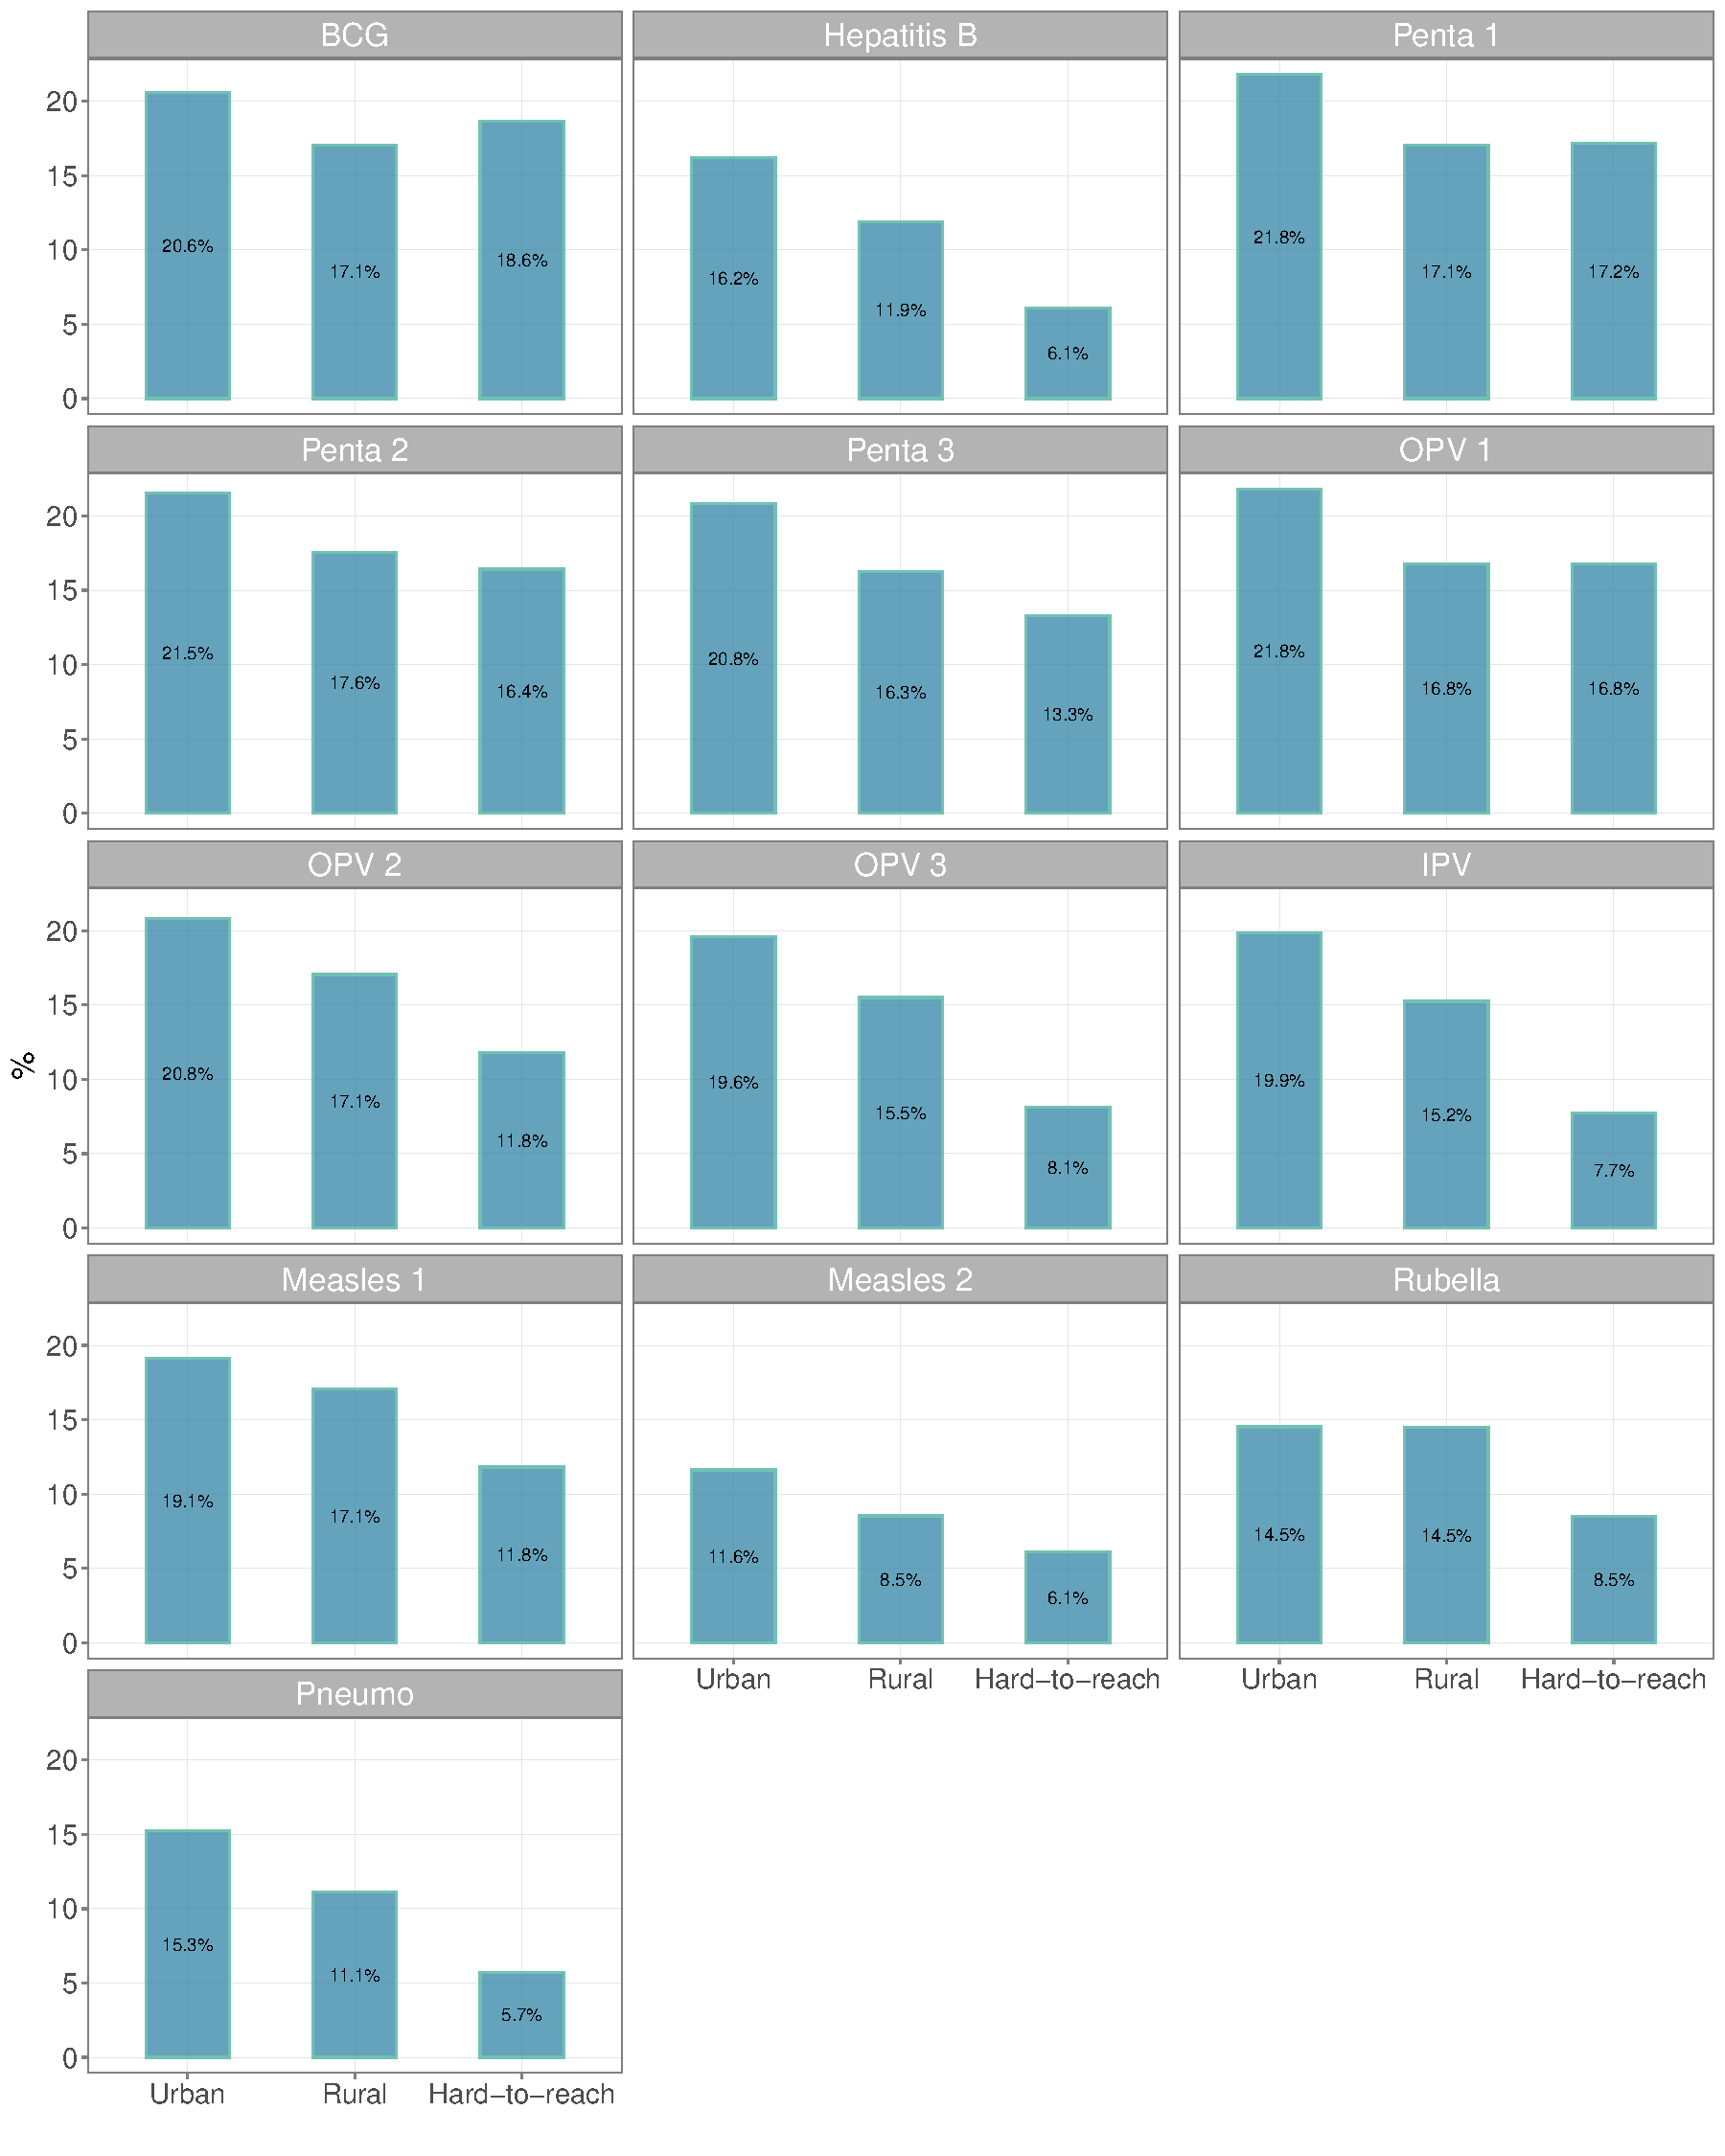
\includegraphics{kayahReport_files/figure-latex/epi3plot-1} 

}

\caption{Immunisation coverage per vaccine by location type}\label{fig:epi3plot}
\end{figure}

\begin{figure}[H]

{\centering 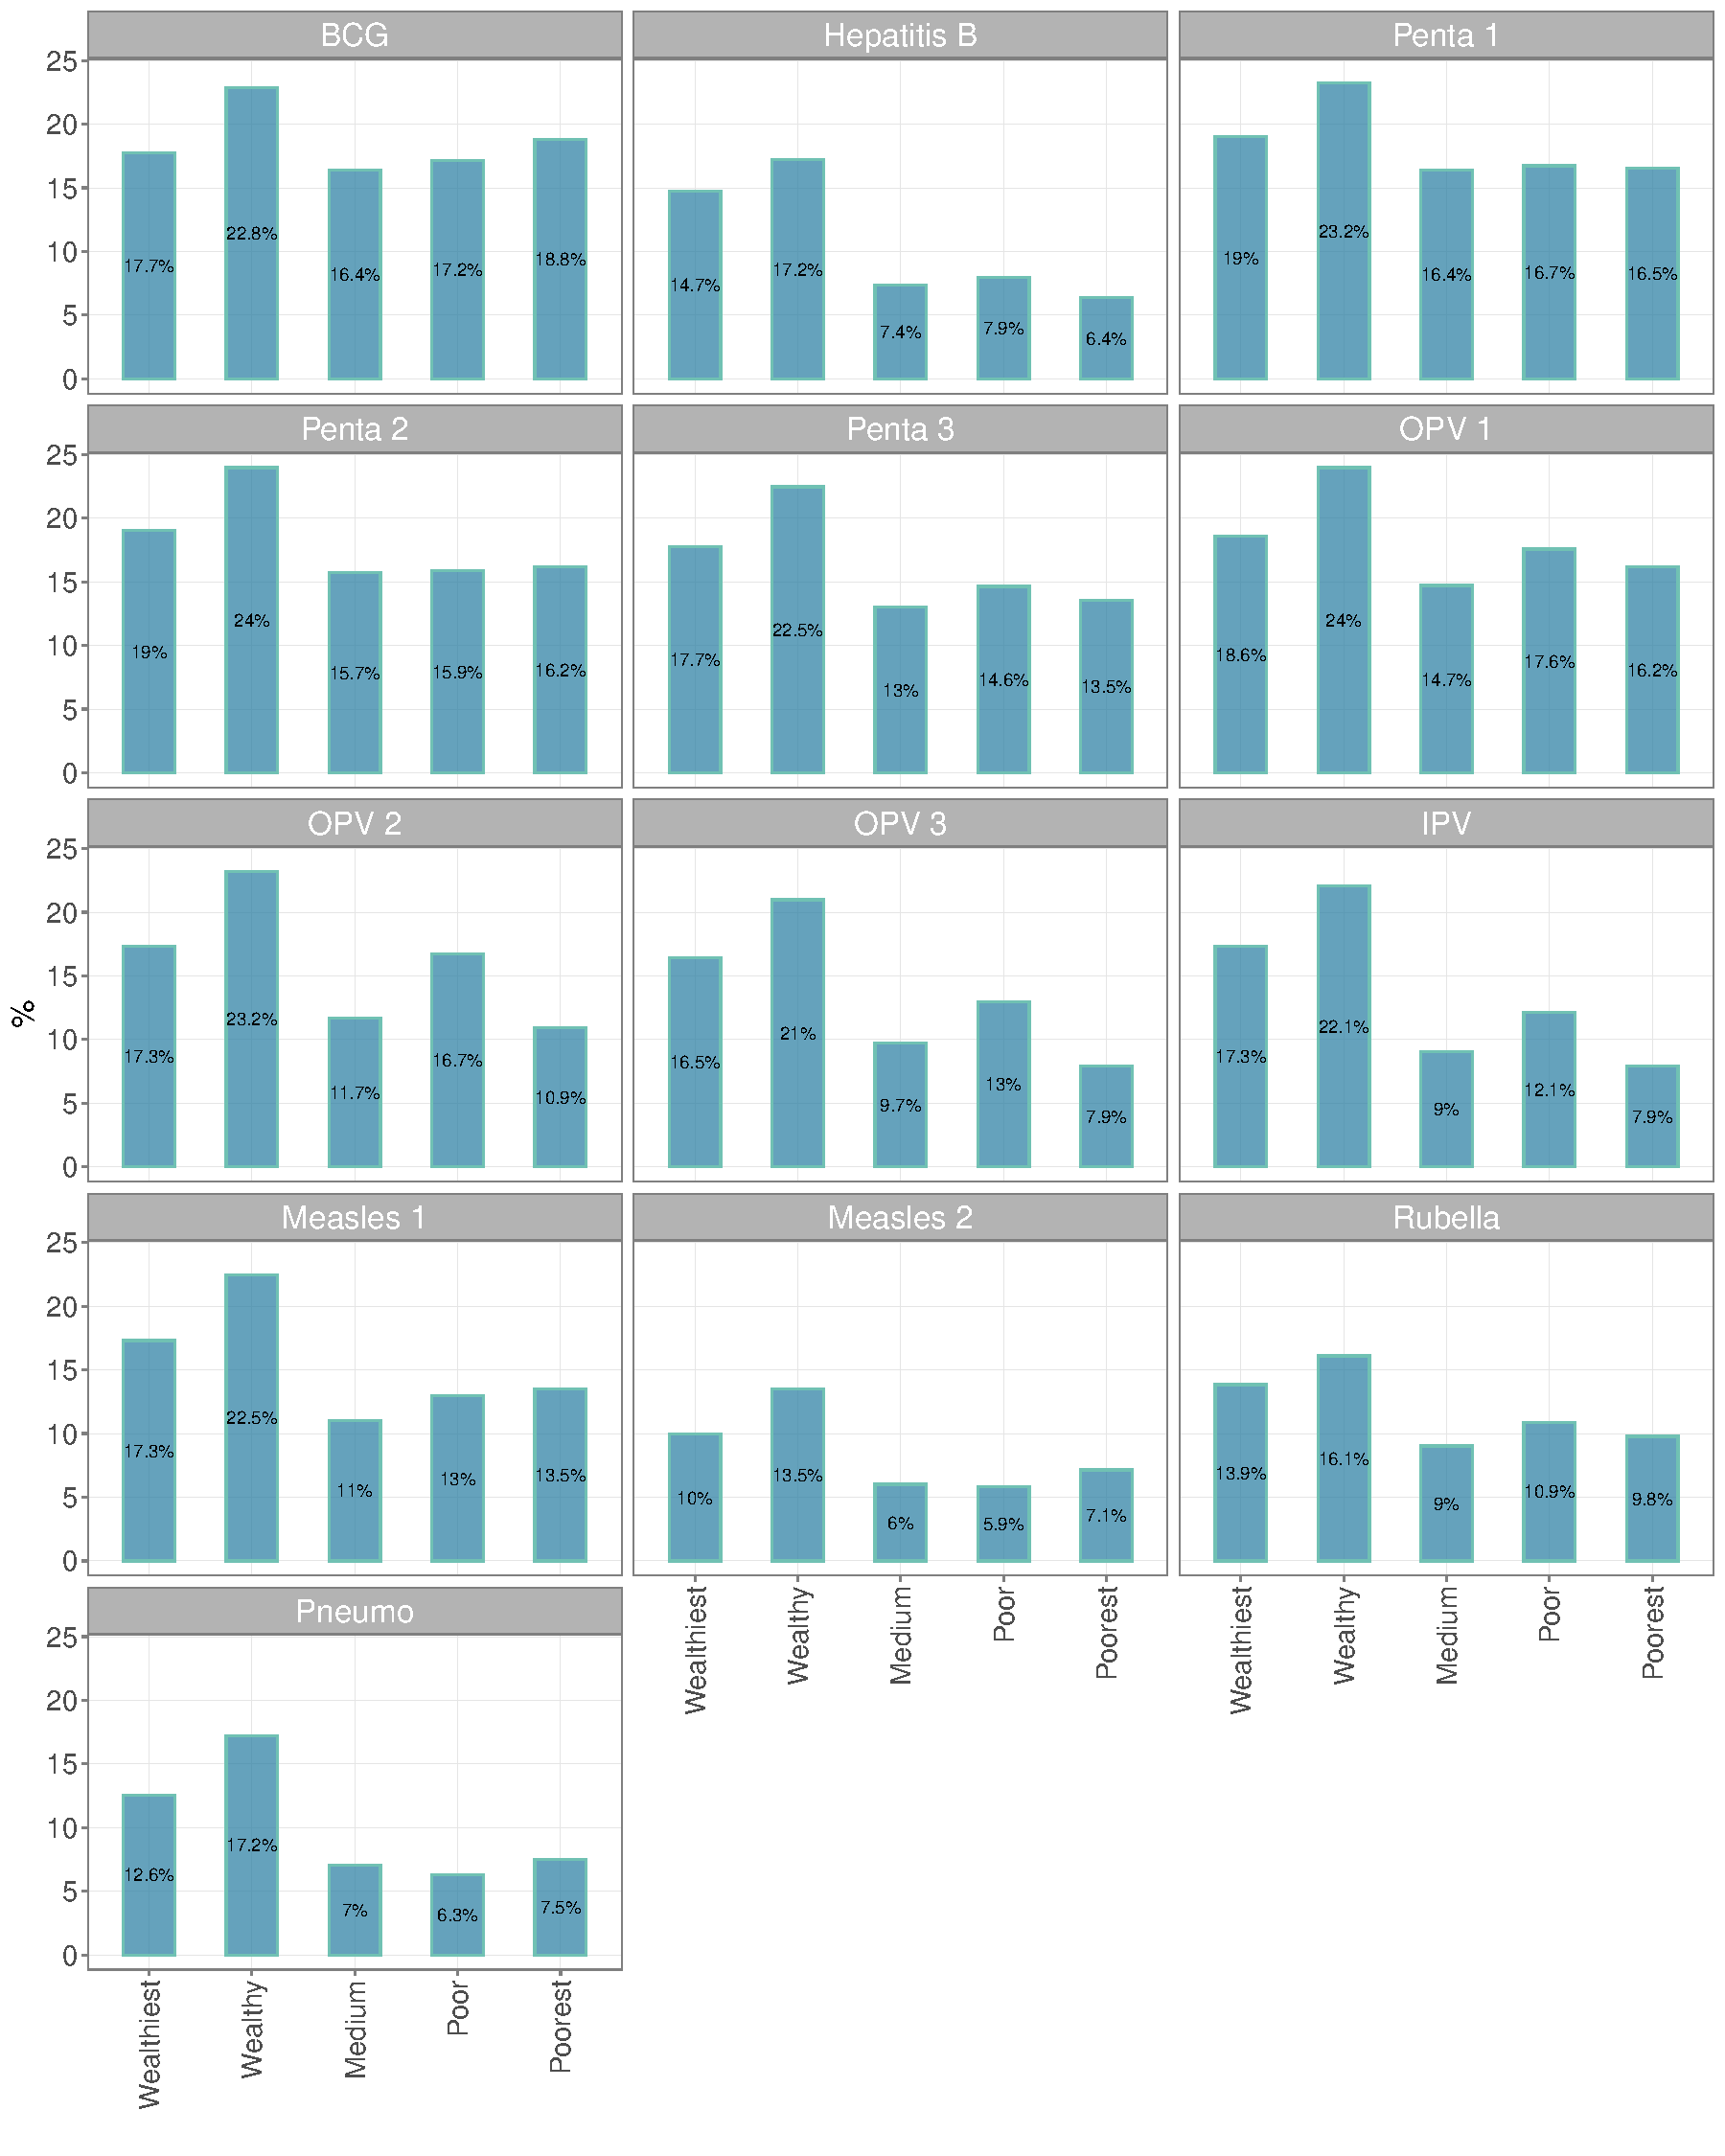
\includegraphics{kayahReport_files/figure-latex/epi4plot-1} 

}

\caption{Immunisation coverage per vaccine by wealth quintiles}\label{fig:epi4plot}
\end{figure}

\begin{table}[H]

\caption{\label{tab:epi3table}Coverage of immunisation-associated services}
\centering
\fontsize{12}{14}\selectfont
\begin{tabular}[t]{>{\bfseries}l>{\bfseries}l>{\ttfamily}r>{\ttfamily}r}
\toprule
 &  & \makecell[c]{Vitamin\\A\\supplementation\\(\%)} & \makecell[c]{Deworming\\(\%)}\\
\midrule
\addlinespace[0.3em]
\multicolumn{4}{l}{\textbf{Kayah}}\\
\addlinespace[0.3em]
\multicolumn{4}{l}{\textit{\textbf{Geographic}}}\\
\hspace{1em}\hspace{1em} & Rural & 56.5 & 24.9\\
\cmidrule{2-4}
\hspace{1em}\hspace{1em} & Urban & 35.8 & 10.9\\
\cmidrule{2-4}
\hspace{1em}\hspace{1em} & Hard-to-reach & 26.5 & 13.8\\
\cmidrule{2-4}
\addlinespace[0.3em]
\multicolumn{4}{l}{\textit{\textbf{Wealth}}}\\
\hspace{1em}\hspace{1em} & Wealthiest & 33.6 & 11.5\\
\cmidrule{2-4}
\hspace{1em}\hspace{1em} & Wealthy & 40.3 & 15.5\\
\cmidrule{2-4}
\hspace{1em}\hspace{1em} & Medium & 40.2 & 15.6\\
\cmidrule{2-4}
\hspace{1em}\hspace{1em} & Poor & 41.1 & 15.9\\
\cmidrule{2-4}
\hspace{1em}\hspace{1em} & Poorest & 36.6 & 22.0\\
\bottomrule
\end{tabular}
\end{table}

\begin{figure}[H]

{\centering 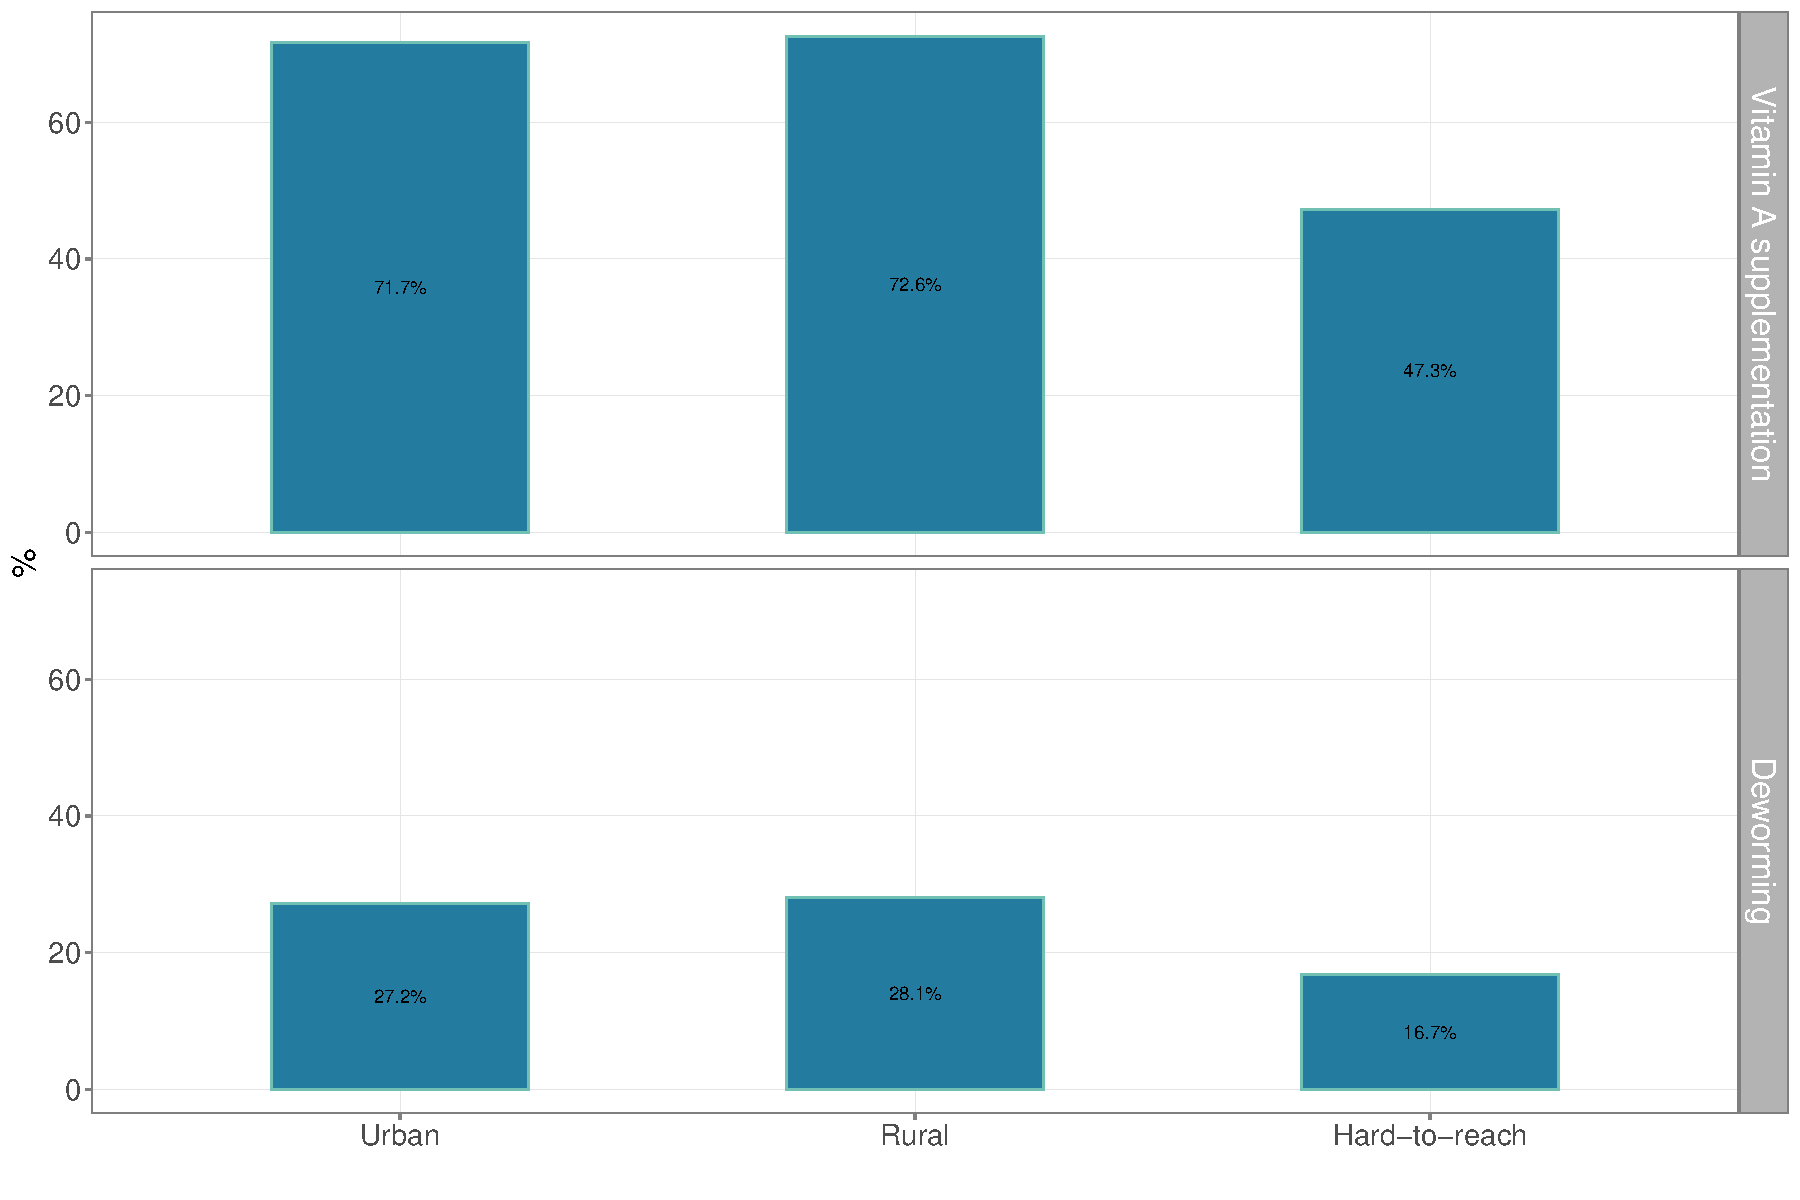
\includegraphics{kayahReport_files/figure-latex/epi5plot-1} 

}

\caption{Immunisation-associated services coverage by location type}\label{fig:epi5plot}
\end{figure}

\begin{figure}[H]

{\centering 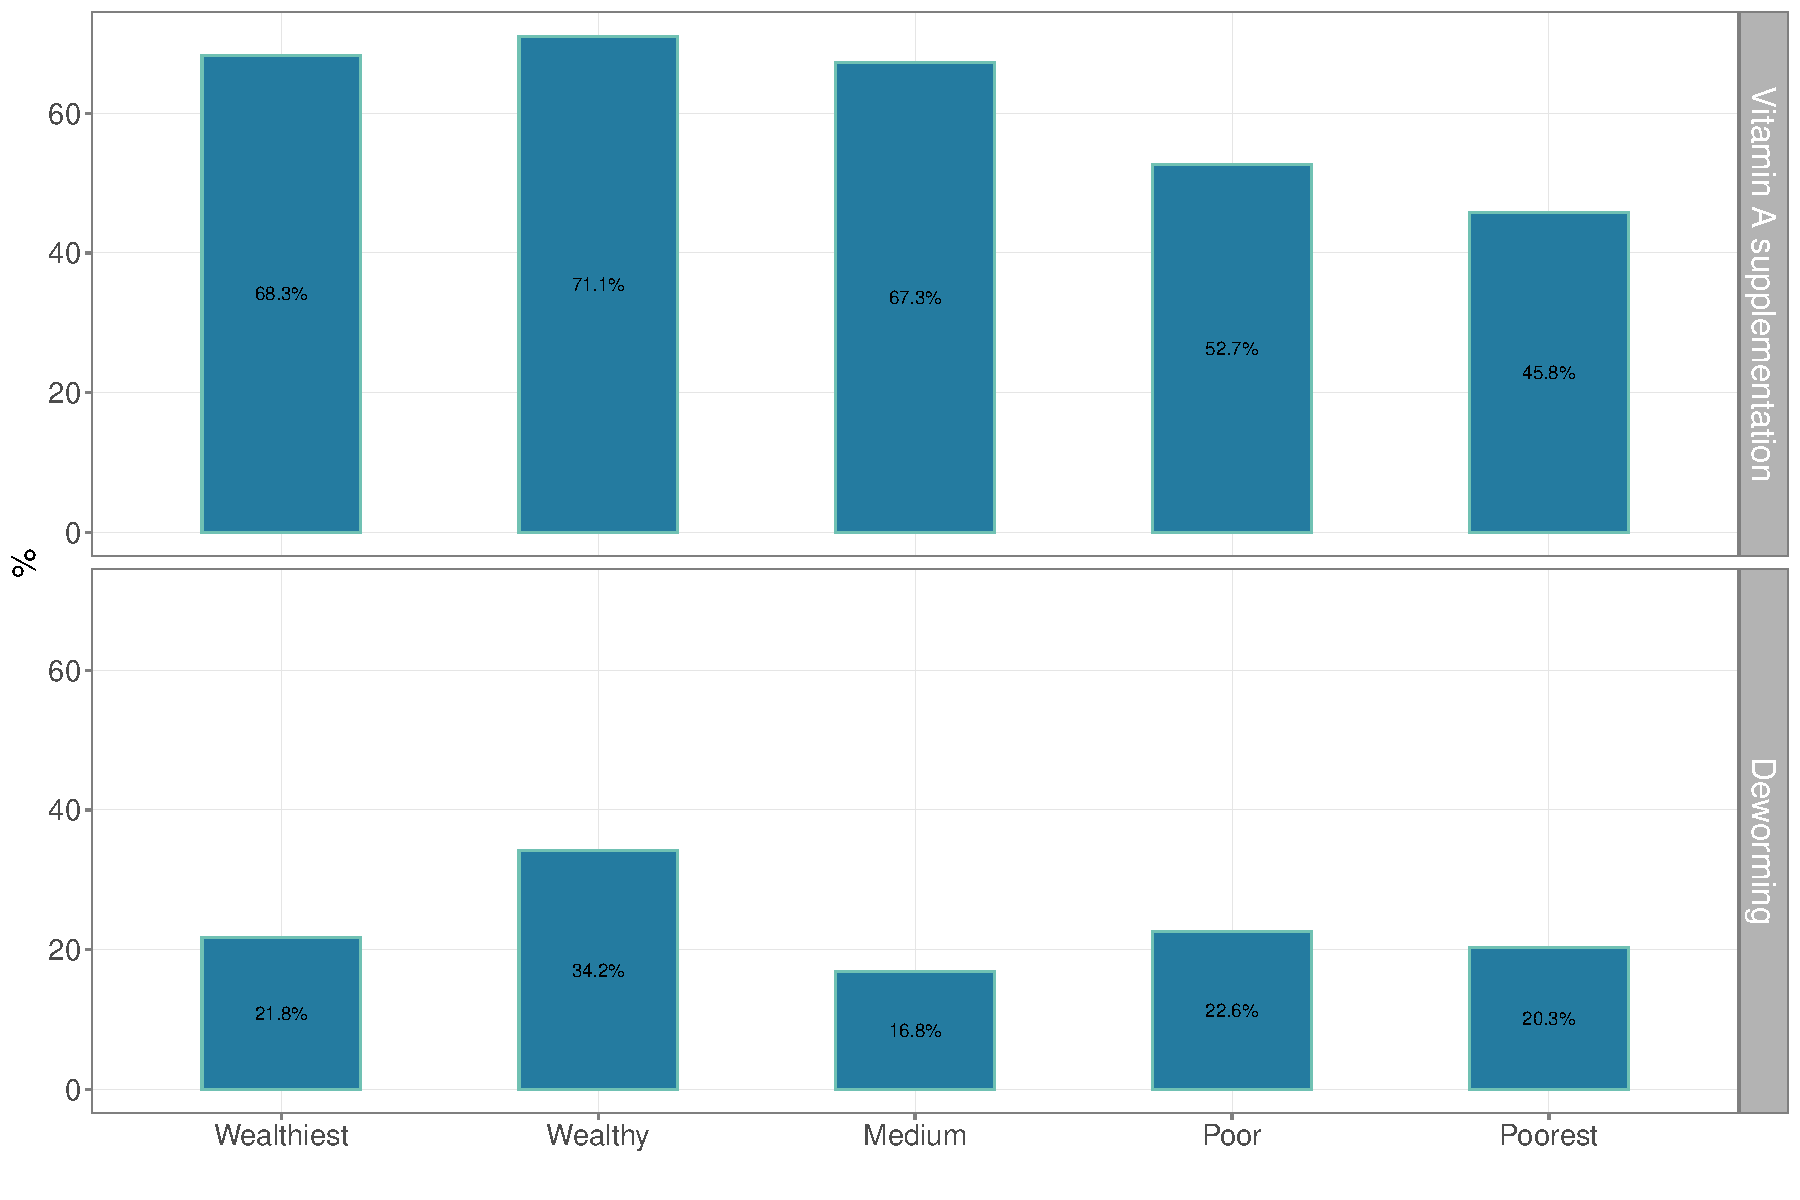
\includegraphics{kayahReport_files/figure-latex/epi6plot-1} 

}

\caption{Immunisation-associated services coverage by wealth quintiles}\label{fig:epi6plot}
\end{figure}

\hypertarget{illness}{%
\subsubsection{Period prevalence of childhood illnesses}\label{illness}}

\begin{table}[H]

\caption{\label{tab:ill1table}Period prevalence of childhood illnesses}
\centering
\fontsize{12}{14}\selectfont
\begin{tabular}[t]{>{\bfseries}l>{\bfseries}l>{\ttfamily}r>{\ttfamily}r>{\ttfamily}r}
\toprule
 &  & \makecell[c]{Diarrhoea\\(\%)} & \makecell[c]{ARI\\(\%)} & \makecell[c]{Fever\\(\%)}\\
\midrule
\addlinespace[0.3em]
\multicolumn{5}{l}{\textbf{Kayah}}\\
\addlinespace[0.3em]
\multicolumn{5}{l}{\textit{\textbf{Geographic}}}\\
\hspace{1em}\hspace{1em} & Rural & 3.2 & 9.0 & 28.5\\
\cmidrule{2-5}
\hspace{1em}\hspace{1em} & Urban & 1.6 & 8.1 & 25.8\\
\cmidrule{2-5}
\hspace{1em}\hspace{1em} & Hard-to-reach & 2.9 & 11.3 & 18.0\\
\cmidrule{2-5}
\addlinespace[0.3em]
\multicolumn{5}{l}{\textit{\textbf{Wealth}}}\\
\hspace{1em}\hspace{1em} & Wealthiest & 2.0 & 8.9 & 27.1\\
\cmidrule{2-5}
\hspace{1em}\hspace{1em} & Wealthy & 1.1 & 7.9 & 27.1\\
\cmidrule{2-5}
\hspace{1em}\hspace{1em} & Medium & 2.3 & 8.9 & 27.1\\
\cmidrule{2-5}
\hspace{1em}\hspace{1em} & Poor & 2.7 & 10.8 & 18.8\\
\cmidrule{2-5}
\hspace{1em}\hspace{1em} & Poorest & 4.7 & 9.9 & 20.6\\
\bottomrule
\end{tabular}
\end{table}

\begin{figure}[H]

{\centering 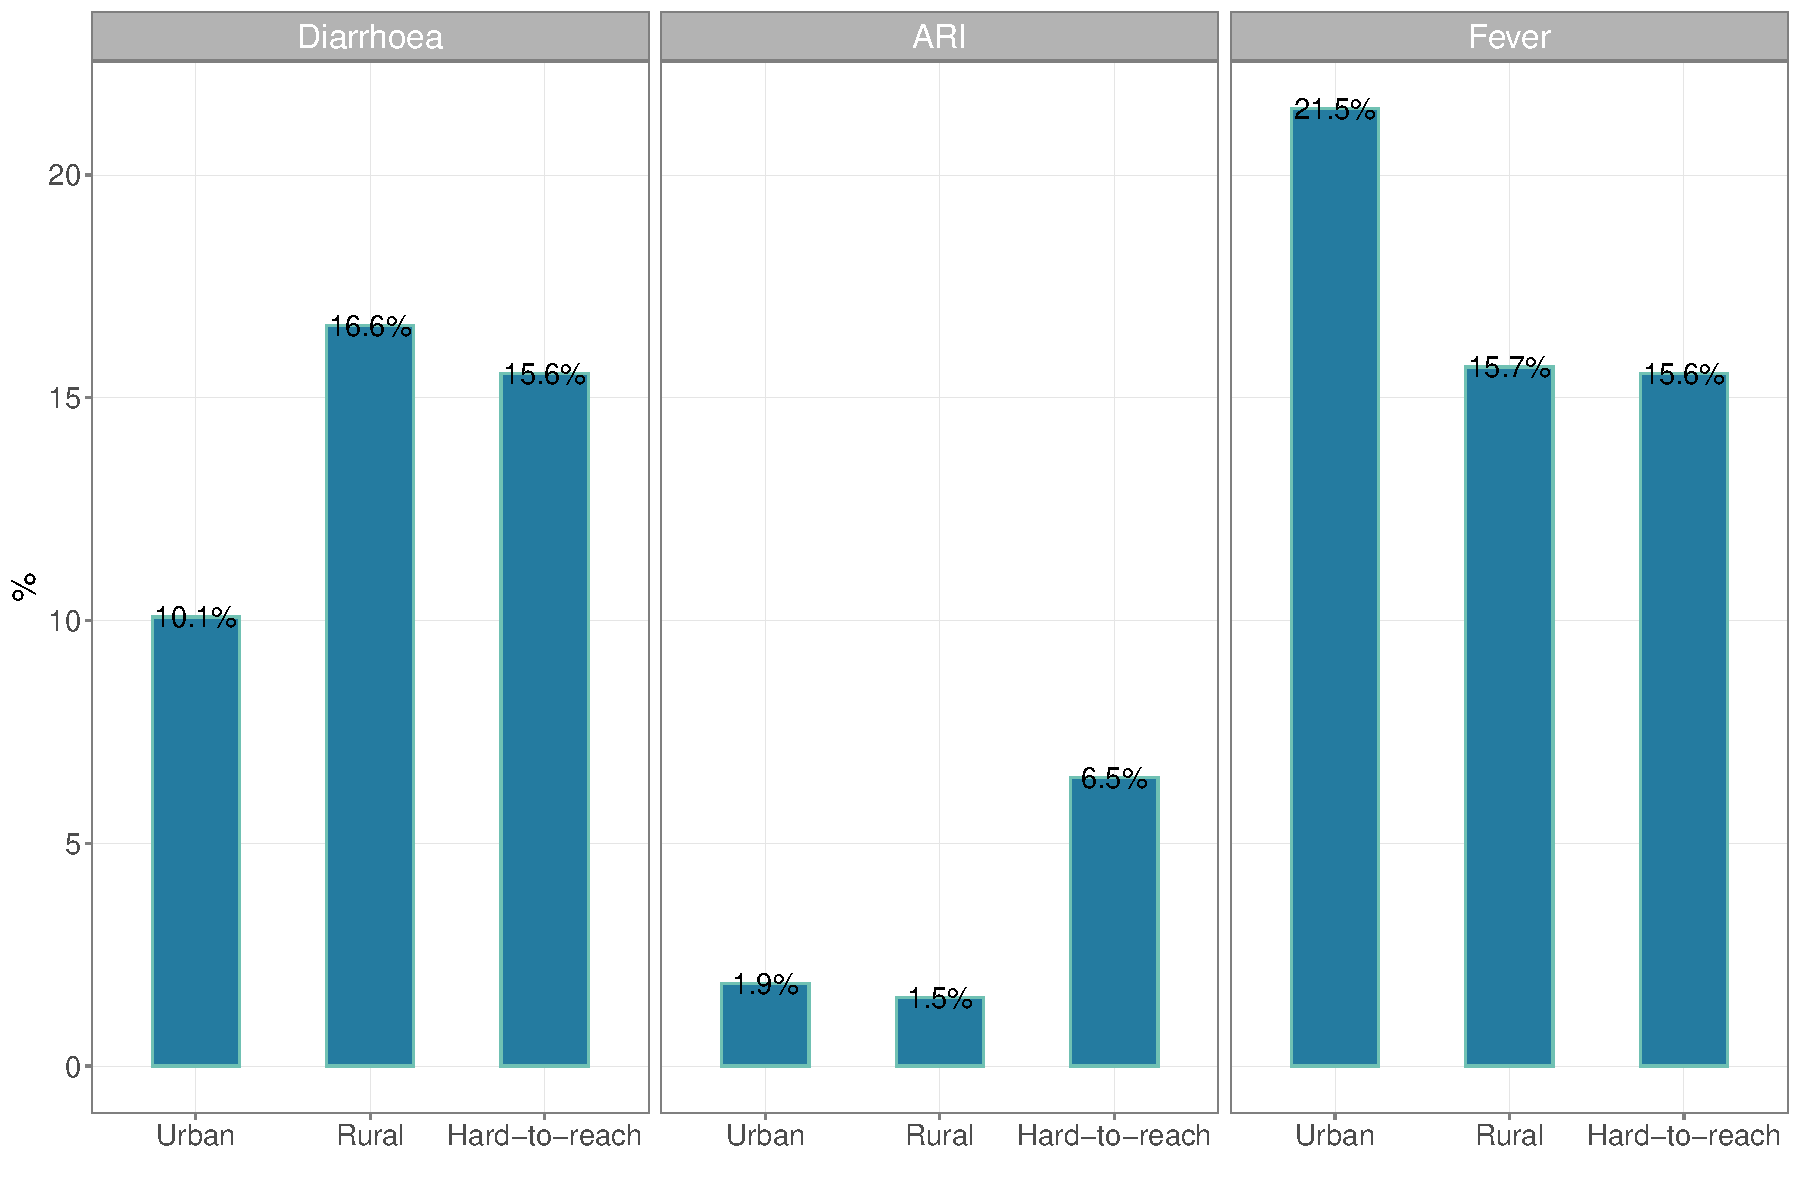
\includegraphics{kayahReport_files/figure-latex/ill1plot-1} 

}

\caption{Period prevalence of childhood illnesses by location type}\label{fig:ill1plot}
\end{figure}

\begin{figure}[H]

{\centering 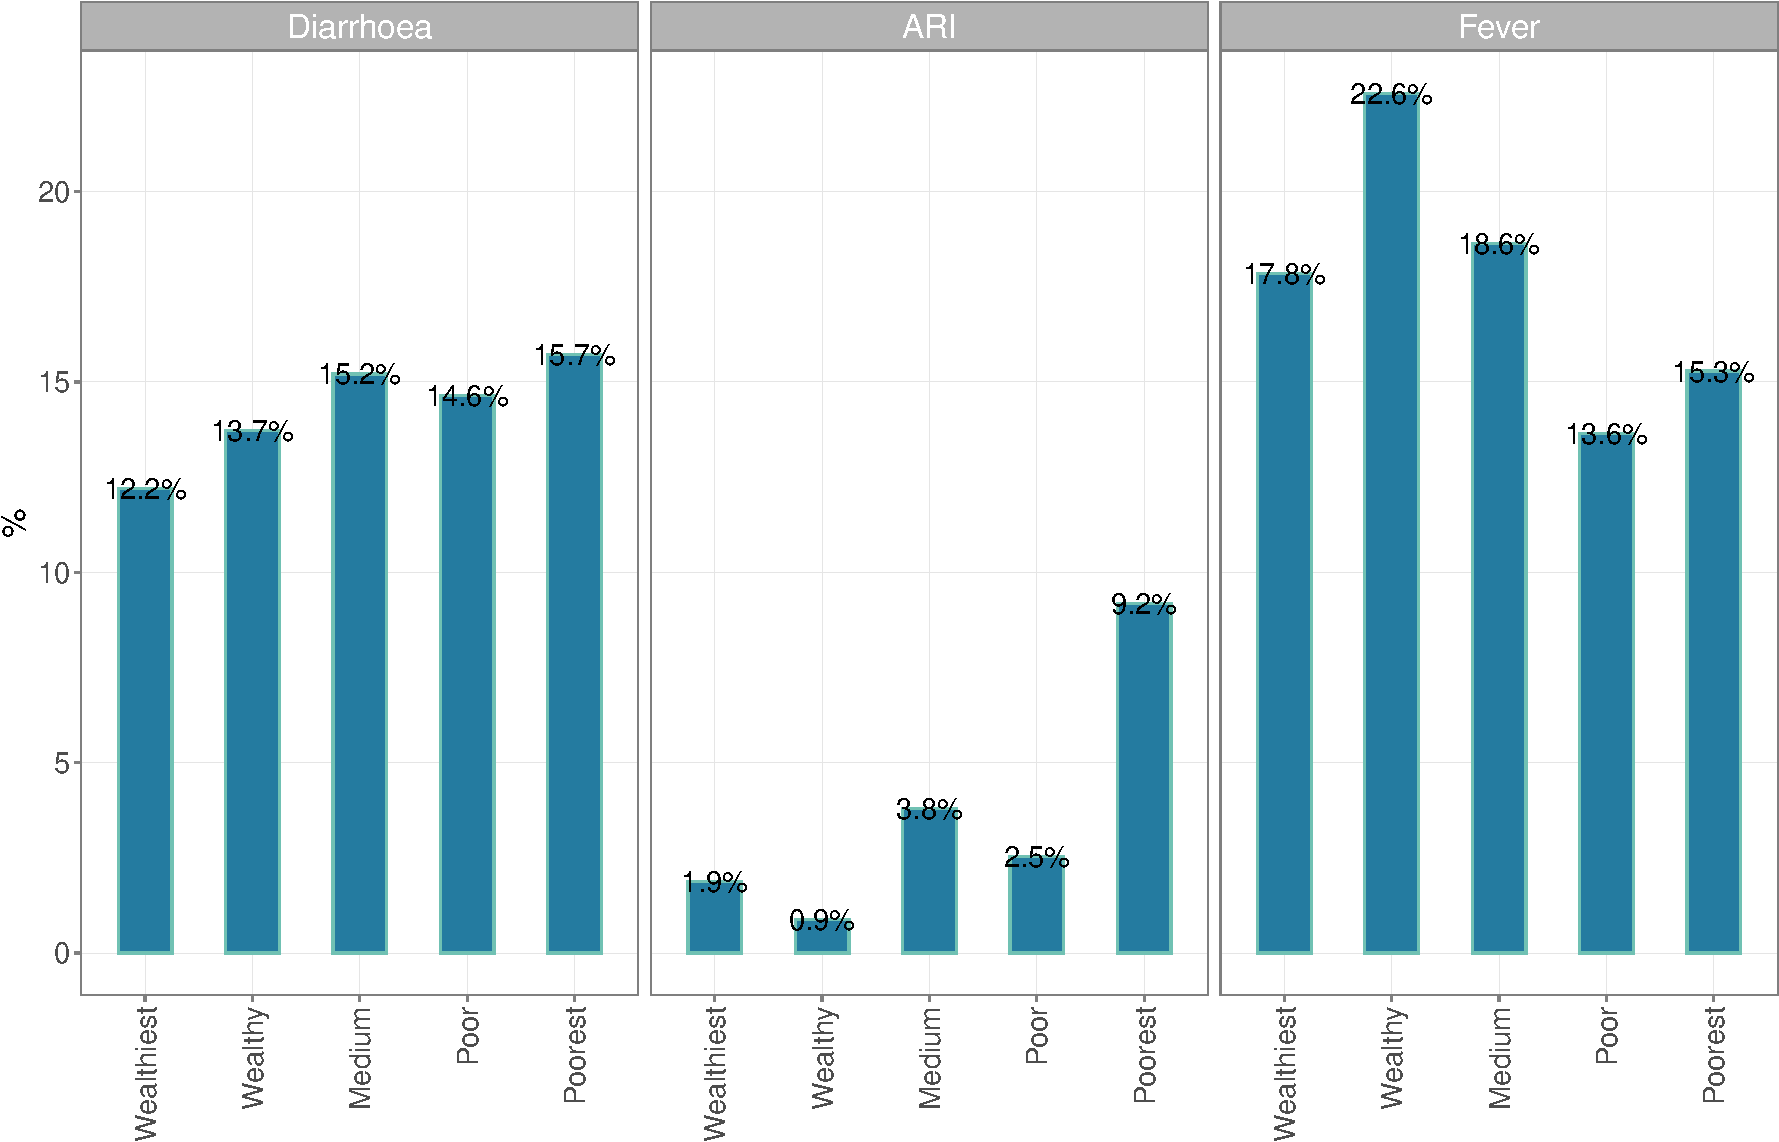
\includegraphics{kayahReport_files/figure-latex/ill2plot-1} 

}

\caption{Period prevalence of childhood illnesses by wealth quintiles}\label{fig:ill2plot}
\end{figure}

\hypertarget{ctreatment}{%
\subsubsection{Treatment-seeking behaviour}\label{ctreatment}}

\hypertarget{diarrhoea}{%
\paragraph{Diarrhoea}\label{diarrhoea}}

\begin{landscape}\begin{table}[H]

\caption{\label{tab:diarrhoea1table}Treatment-seeking for diarrhoea}
\centering
\fontsize{10}{12}\selectfont
\begin{tabular}[t]{>{\bfseries}l>{\bfseries}l>{\ttfamily}r>{\ttfamily}r>{\ttfamily}r>{\ttfamily}r>{\ttfamily}r>{\ttfamily}r>{\ttfamily}r>{\ttfamily}r>{\ttfamily}r}
\toprule
\multicolumn{4}{c}{\textbf{ }} & \multicolumn{7}{c}{\textbf{Reasons for not seeking treatment}} \\
\cmidrule(l{3pt}r{3pt}){5-11}
 &  & \makecell[c]{Sought\\treatment\\(\%)} & \makecell[c]{Time to\\treatment\\(days)} & \makecell[c]{No\\facility\\(\%)} & \makecell[c]{Facility\\inaccessible\\(\%)} & \makecell[c]{Expensive\\(\%)} & \makecell[c]{Not\\necessary\\(\%)} & \makecell[c]{Advised\\not to\\(\%)} & \makecell[c]{Alternative\\treatment\\(\%)} & \makecell[c]{Do not know\\treamtent\\(\%)}\\
\midrule
\addlinespace[0.3em]
\multicolumn{11}{l}{\textbf{Kayah}}\\
\addlinespace[0.3em]
\multicolumn{11}{l}{\textit{\textbf{Geographic}}}\\
\hspace{1em}\hspace{1em} & Rural & 76.9 & 1.2 & 0 & 14.3 & 0.0 & 0.0 & 0 & 42.9 & 0\\
\cmidrule{2-11}
\hspace{1em}\hspace{1em} & Urban & 87.5 & 1.1 & 0 & 0.0 & 33.3 & 33.3 & 0 & 0.0 & 0\\
\cmidrule{2-11}
\hspace{1em}\hspace{1em} & Hard-to-reach & 80.0 & 1.3 & 0 & 0.0 & 50.0 & 0.0 & 0 & 0.0 & 0\\
\cmidrule{2-11}
\addlinespace[0.3em]
\multicolumn{11}{l}{\textit{\textbf{Wealth}}}\\
\hspace{1em}\hspace{1em} & Wealthiest & 80.0 & 1.0 & 0 & 0.0 & 50.0 & 0.0 & 0 & 0.0 & 0\\
\cmidrule{2-11}
\hspace{1em}\hspace{1em} & Wealthy & 100.0 & 1.3 & NaN & NaN & NaN & NaN & NaN & NaN & NaN\\
\cmidrule{2-11}
\hspace{1em}\hspace{1em} & Medium & 100.0 & 1.2 & 0 & 0.0 & 0.0 & 0.0 & 0 & 0.0 & 0\\
\cmidrule{2-11}
\hspace{1em}\hspace{1em} & Poor & 100.0 & 1.3 & 0 & 0.0 & 0.0 & 0.0 & 0 & 100.0 & 0\\
\cmidrule{2-11}
\hspace{1em}\hspace{1em} & Poorest & 54.5 & 1.3 & 0 & 10.0 & 30.0 & 10.0 & 0 & 10.0 & 0\\
\bottomrule
\end{tabular}
\end{table}
\end{landscape}

\begin{figure}[H]

{\centering 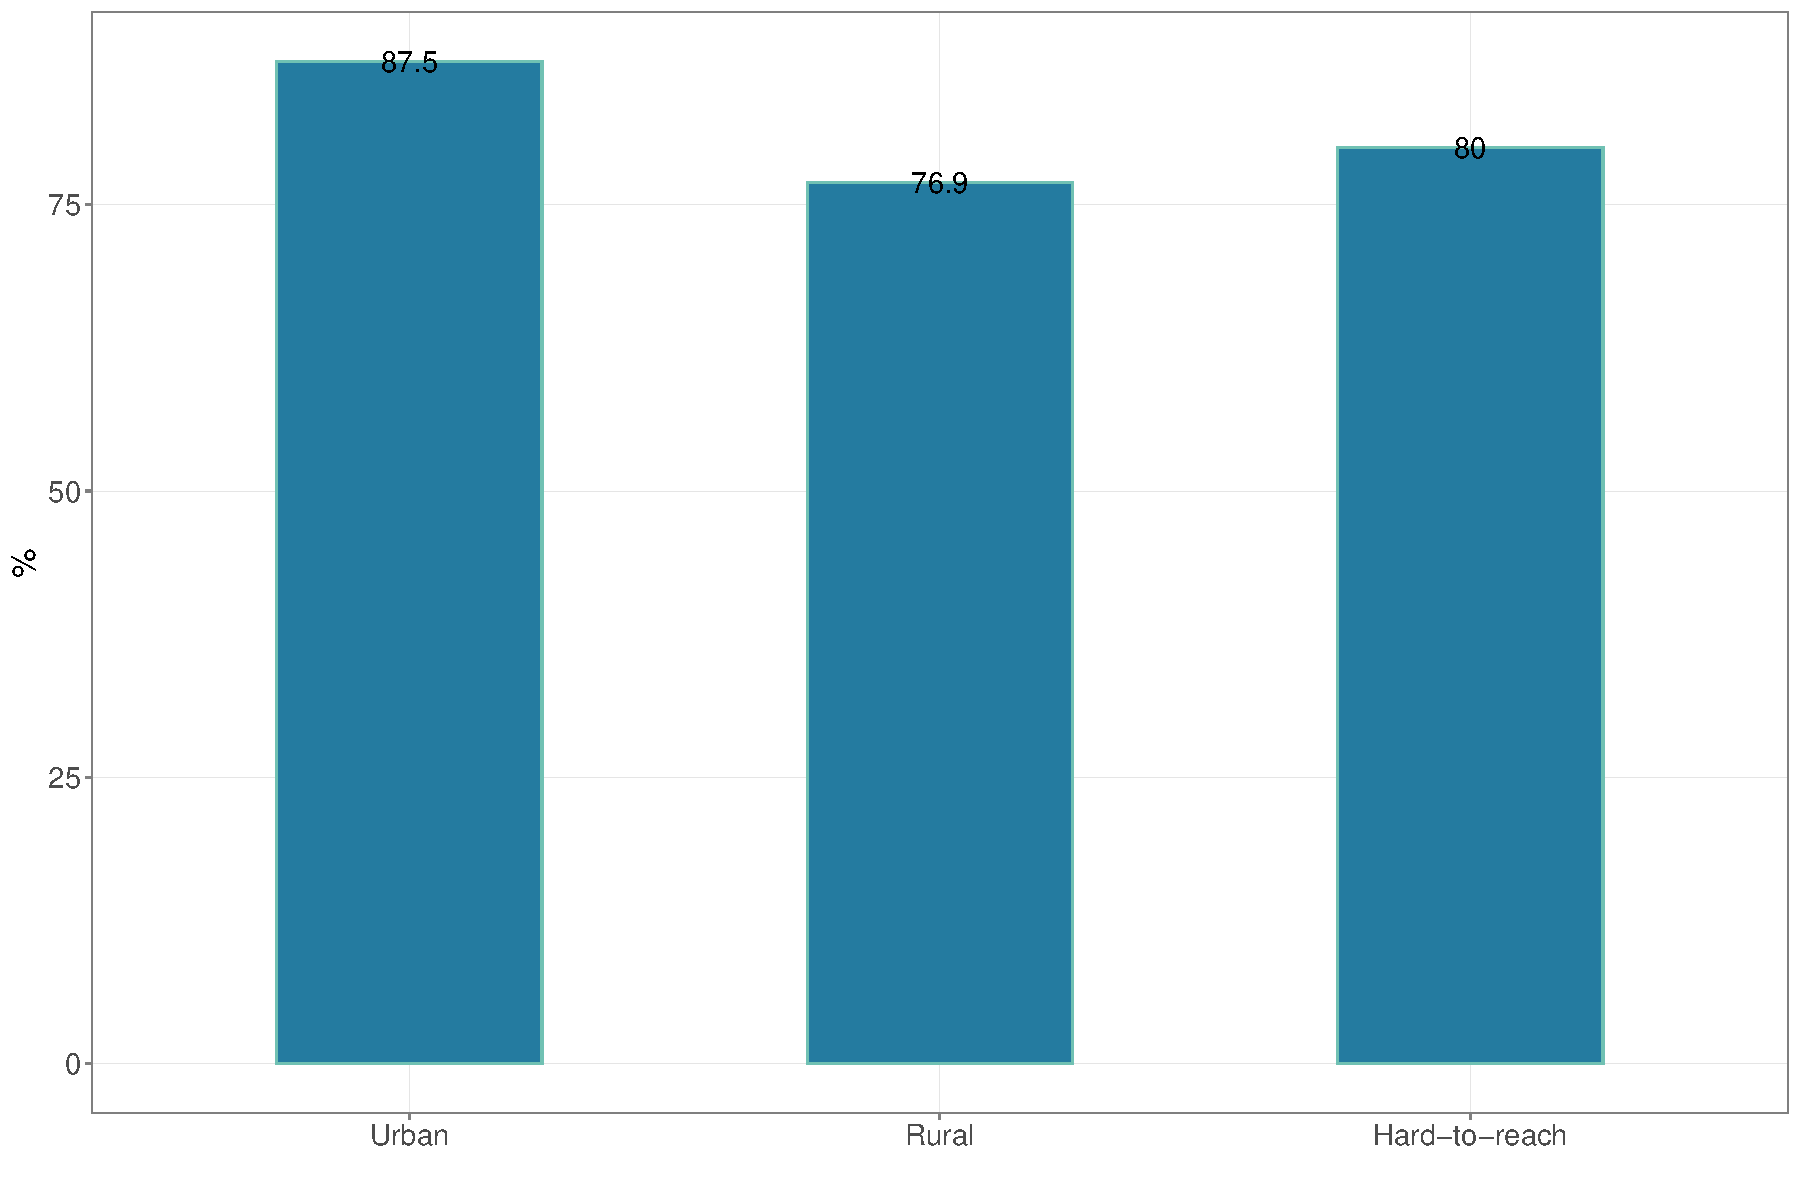
\includegraphics{kayahReport_files/figure-latex/diarrhoea1plot-1} 

}

\caption{Treatment-seeking for diarrhoea by location type}\label{fig:diarrhoea1plot}
\end{figure}

\begin{figure}[H]

{\centering 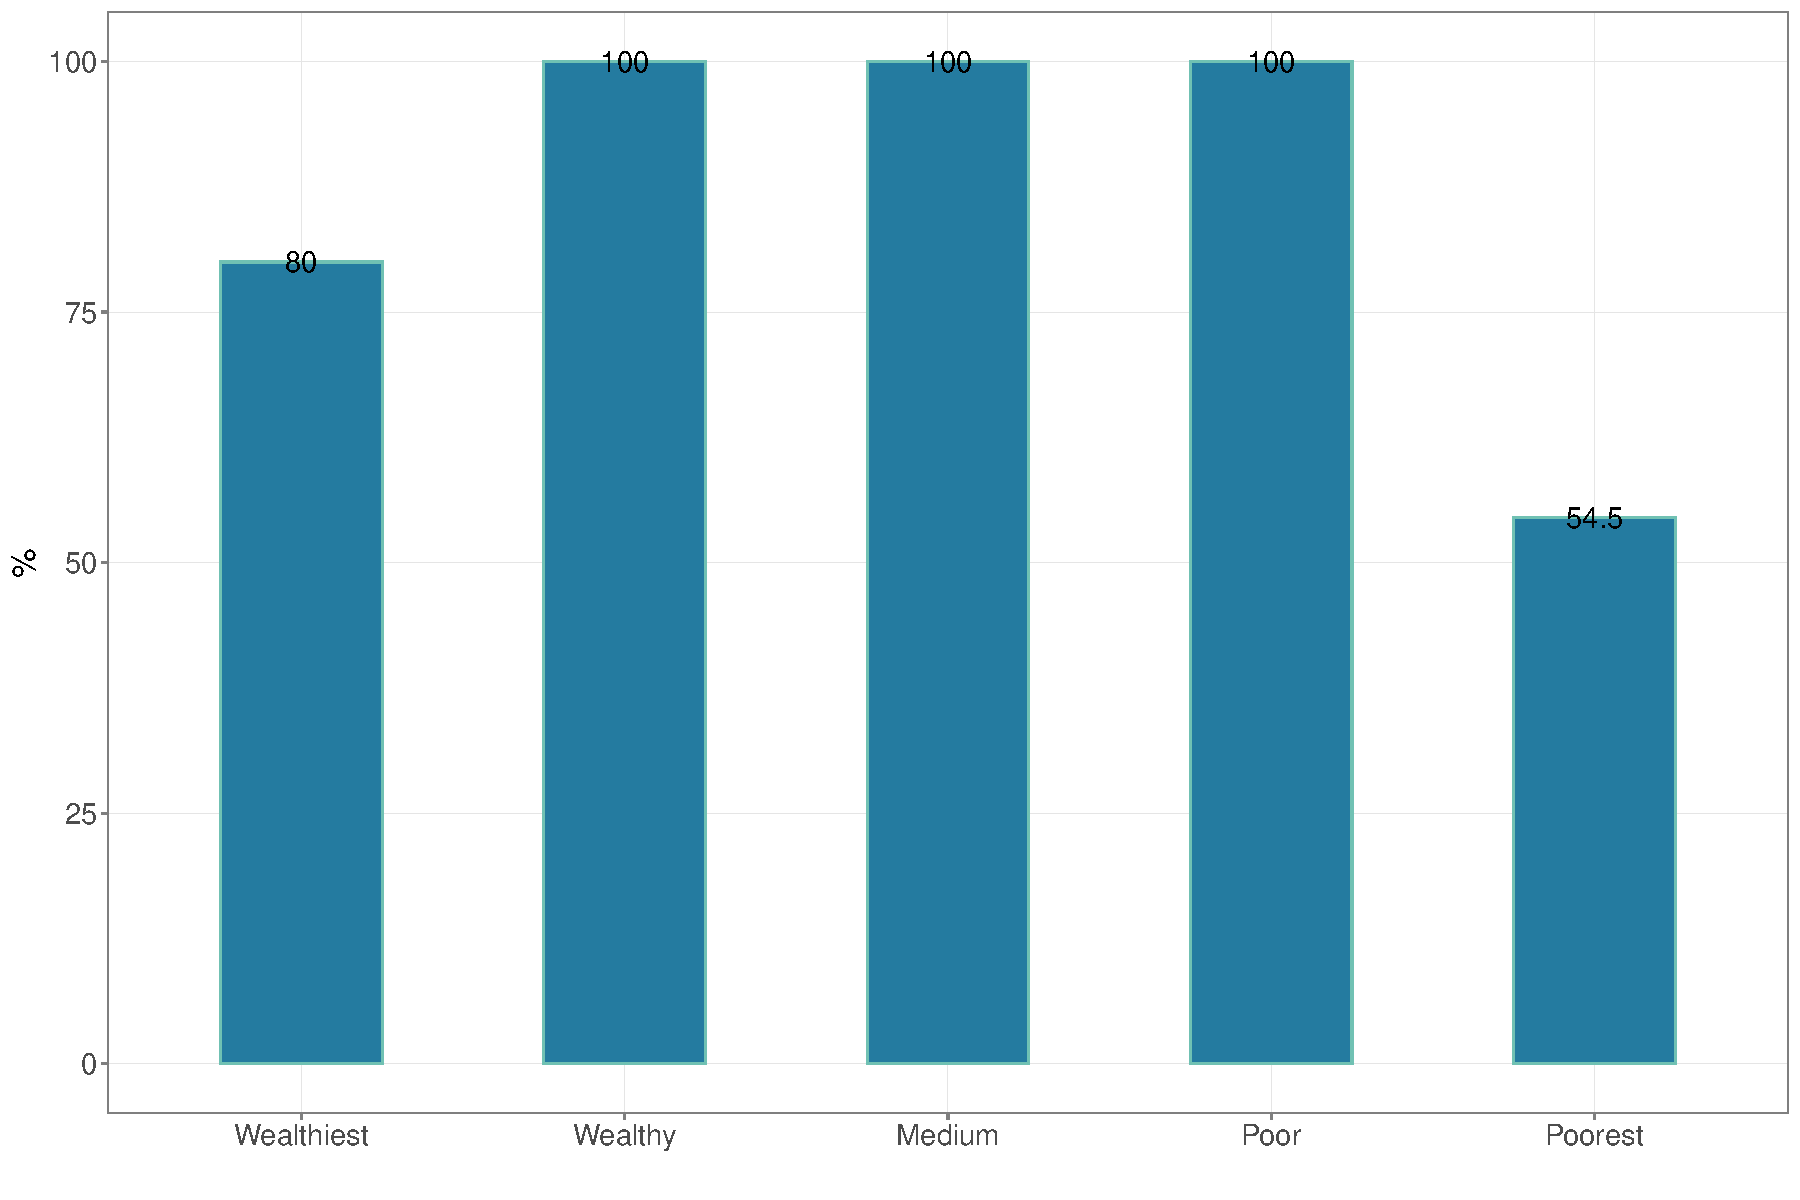
\includegraphics{kayahReport_files/figure-latex/diarrhoea2plot-1} 

}

\caption{Treatment-seeking for diarrhoea by wealth quintiles}\label{fig:diarrhoea2plot}
\end{figure}

\begin{figure}[H]

{\centering 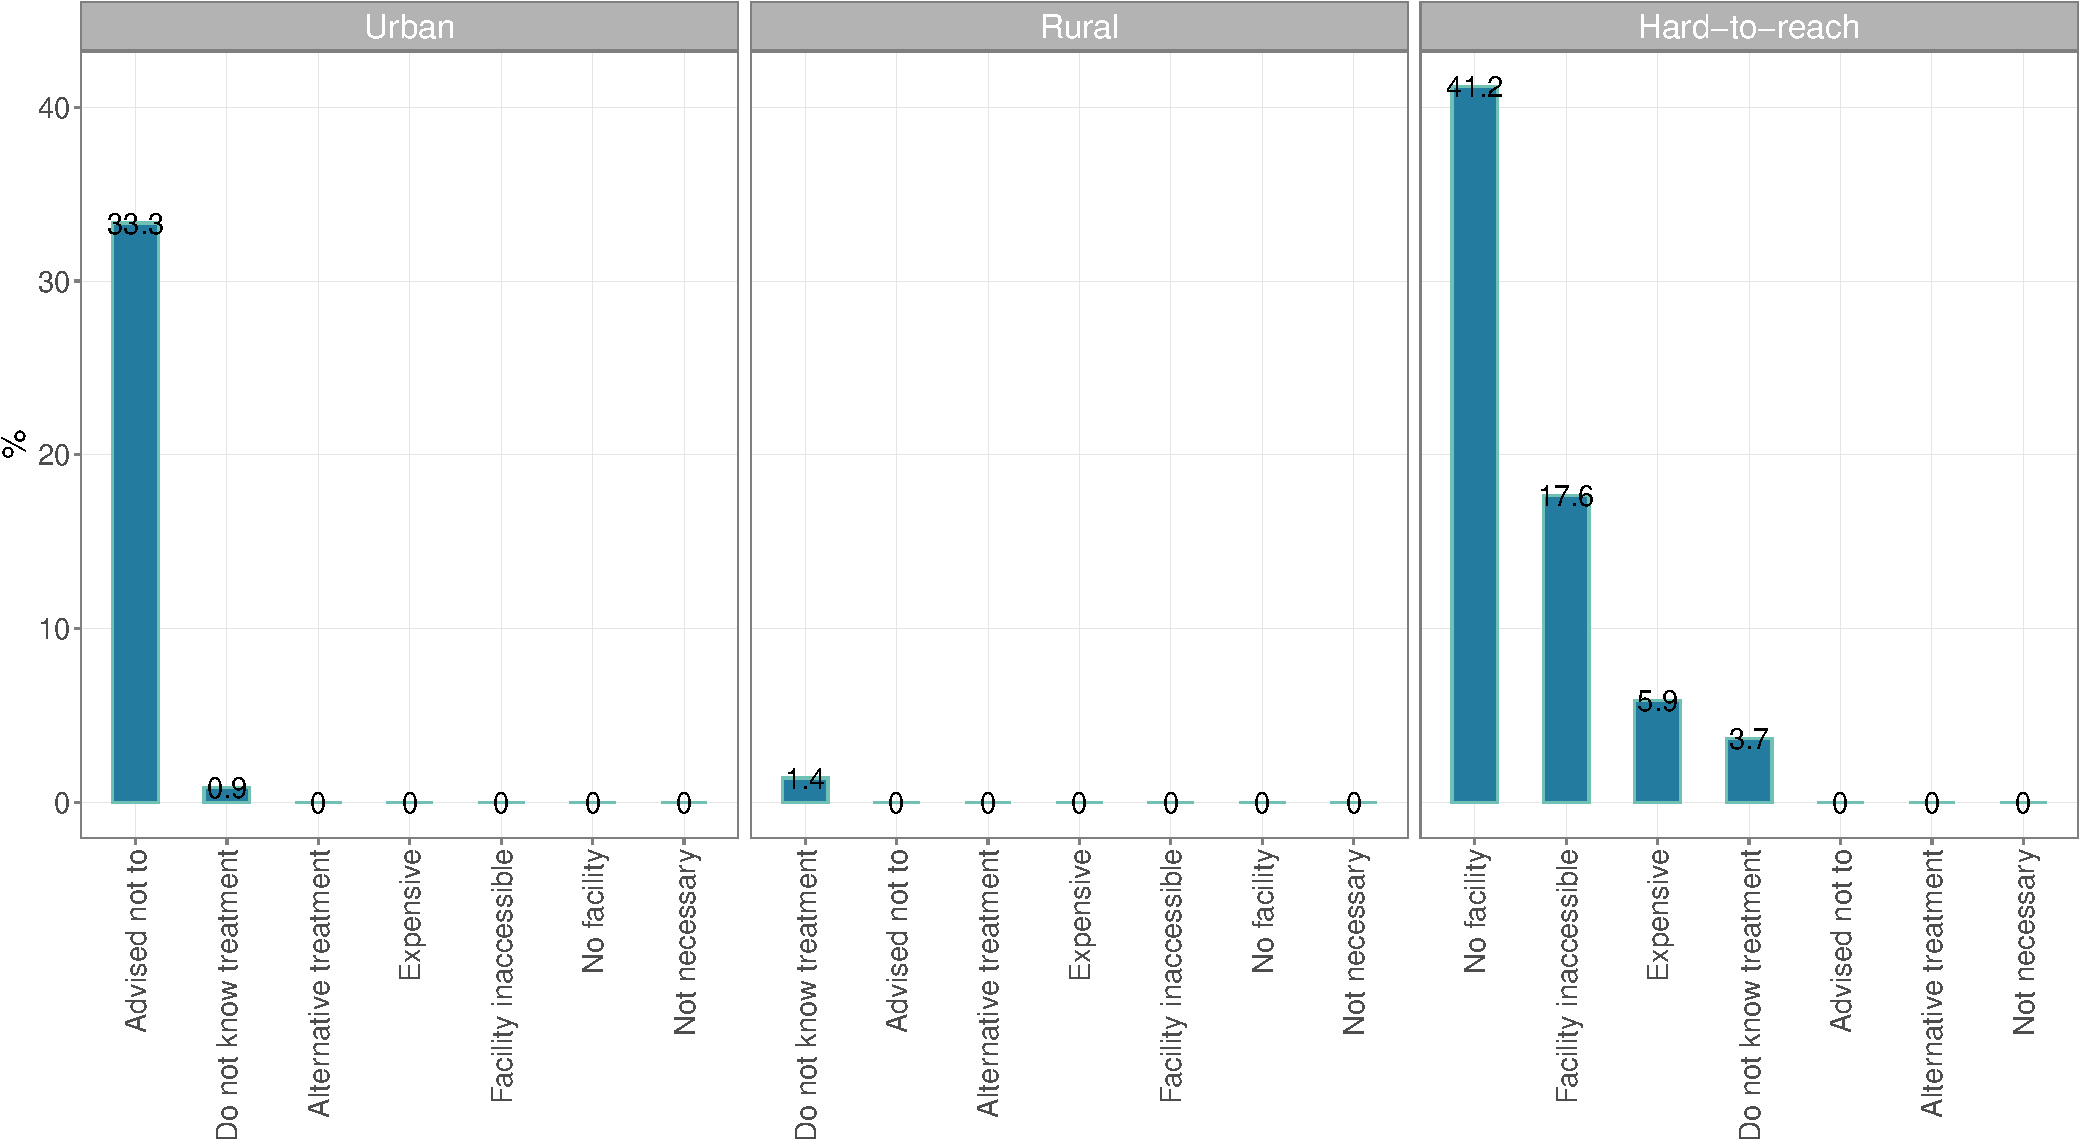
\includegraphics{kayahReport_files/figure-latex/diarrhoea4plot-1} 

}

\caption{Reasons for not seeking treatment by location type}\label{fig:diarrhoea4plot}
\end{figure}

\begin{landscape}\begin{table}[H]

\caption{\label{tab:diarrhoea2table}Where/who treatment is sought from}
\centering
\fontsize{9}{11}\selectfont
\begin{tabular}[t]{>{\bfseries}l>{\bfseries}l>{\ttfamily}r>{\ttfamily}r>{\ttfamily}r>{\ttfamily}r>{\ttfamily}r>{\ttfamily}r>{\ttfamily}r>{\ttfamily}r>{\ttfamily}r>{\ttfamily}r>{\ttfamily}r>{\ttfamily}r>{\ttfamily}r}
\toprule
\multicolumn{2}{c}{\textbf{ }} & \multicolumn{13}{c}{\textbf{Where/who treatment is sought from}} \\
\cmidrule(l{3pt}r{3pt}){3-15}
 &  & \makecell[c]{Township\\hospital\\(\%)} & \makecell[c]{Station\\hospital\\(\%)} & \makecell[c]{RHC/\\health\\assistant\\(\%)} & \makecell[c]{SRHC/\\midwife\\(\%)} & \makecell[c]{Private\\clinic/\\doctor\\(\%)} & \makecell[c]{Community\\health\\worker\\(\%)} & \makecell[c]{Traditional\\healer\\(\%)} & \makecell[c]{Untrained\\health\\worker\\(\%)} & \makecell[c]{Drug\\from\\shop\\(\%)} & \makecell[c]{EHO\\clinic/\\volunteer\\(\%)} & \makecell[c]{Family\\member\\(\%)} & \makecell[c]{NGOs/\\clinic\\(\%)} & \makecell[c]{Auxilliary\\midwife\\(\%)}\\
\midrule
\addlinespace[0.3em]
\multicolumn{15}{l}{\textbf{Kayah}}\\
\addlinespace[0.3em]
\multicolumn{15}{l}{\textit{\textbf{Geographic}}}\\
\hspace{1em}\hspace{1em} & Rural & 11.1 & 5.6 & 22.2 & 22.2 & 0.0 & 5.6 & 0.0 & 0.0 & 11.1 & 0.0 & 0.0 & 0 & 11.1\\
\cmidrule{2-15}
\hspace{1em}\hspace{1em} & Urban & 9.1 & 0.0 & 0.0 & 9.1 & 81.8 & 0.0 & 0.0 & 0.0 & 0.0 & 0.0 & 0.0 & 0 & 0.0\\
\cmidrule{2-15}
\hspace{1em}\hspace{1em} & Hard-to-reach & 0.0 & 13.0 & 4.3 & 8.7 & 4.3 & 8.7 & 4.3 & 4.3 & 21.7 & 21.7 & 8.7 & 0 & 0.0\\
\cmidrule{2-15}
\addlinespace[0.3em]
\multicolumn{15}{l}{\textit{\textbf{Wealth}}}\\
\hspace{1em}\hspace{1em} & Wealthiest & 0.0 & 0.0 & 0.0 & 14.3 & 85.7 & 0.0 & 0.0 & 0.0 & 0.0 & 0.0 & 0.0 & 0 & 0.0\\
\cmidrule{2-15}
\hspace{1em}\hspace{1em} & Wealthy & 0.0 & 16.7 & 16.7 & 0.0 & 33.3 & 0.0 & 0.0 & 0.0 & 0.0 & 0.0 & 16.7 & 0 & 0.0\\
\cmidrule{2-15}
\hspace{1em}\hspace{1em} & Medium & 8.3 & 0.0 & 0.0 & 33.3 & 0.0 & 8.3 & 0.0 & 8.3 & 25.0 & 0.0 & 8.3 & 0 & 0.0\\
\cmidrule{2-15}
\hspace{1em}\hspace{1em} & Poor & 7.7 & 15.4 & 23.1 & 7.7 & 7.7 & 0.0 & 7.7 & 0.0 & 7.7 & 15.4 & 0.0 & 0 & 7.7\\
\cmidrule{2-15}
\hspace{1em}\hspace{1em} & Poorest & 0.0 & 7.7 & 7.7 & 7.7 & 7.7 & 15.4 & 0.0 & 0.0 & 23.1 & 23.1 & 0.0 & 0 & 7.7\\
\bottomrule
\end{tabular}
\end{table}
\end{landscape}

\begin{figure}[H]

{\centering 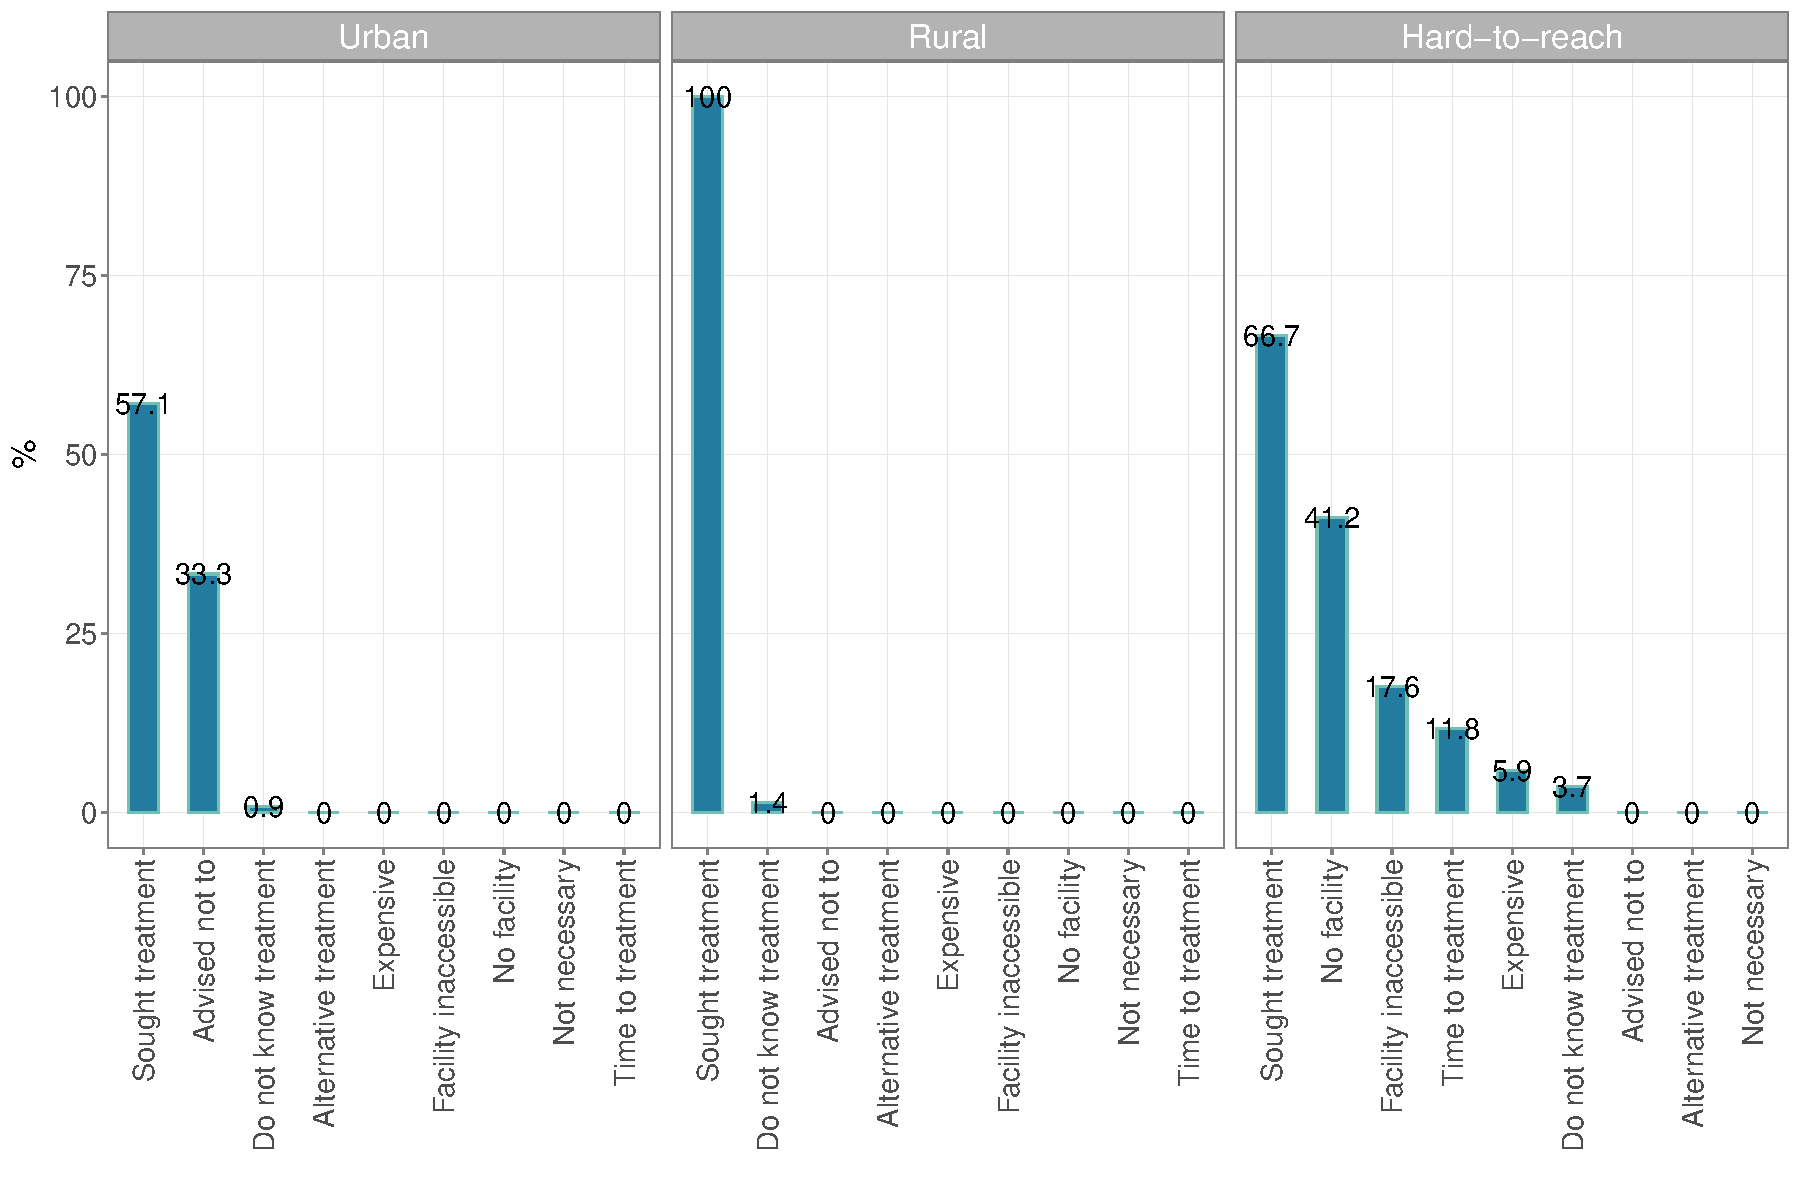
\includegraphics{kayahReport_files/figure-latex/diarrhoea6plot-1} 

}

\caption{Where/who treatment is sought from by location type}\label{fig:diarrhoea6plot}
\end{figure}

\begin{landscape}\begin{table}[H]

\caption{\label{tab:diarrhoea3table}Payment for treatment}
\centering
\fontsize{10}{12}\selectfont
\begin{tabular}[t]{>{\bfseries}l>{\bfseries}l>{\ttfamily}r>{\ttfamily}r>{\ttfamily}r>{\ttfamily}r>{\ttfamily}r>{\ttfamily}r>{\ttfamily}r>{\ttfamily}r}
\toprule
\multicolumn{3}{c}{\textbf{ }} & \multicolumn{6}{c}{\textbf{Payment for}} & \multicolumn{1}{c}{\textbf{ }} \\
\cmidrule(l{3pt}r{3pt}){4-9}
 &  & \makecell[c]{Payment\\for\\service\\(MMK)} & \makecell[c]{Transportation\\(\%)} & \makecell[c]{Registration\\(\%)} & \makecell[c]{Medicine\\(\%)} & \makecell[c]{Laboratory\\fees\\(\%)} & \makecell[c]{Provider\\fees\\(\%)} & \makecell[c]{Gifts\\(\%)} & \makecell[c]{Took\\loan\\(\%)}\\
\midrule
\addlinespace[0.3em]
\multicolumn{10}{l}{\textbf{Kayah}}\\
\addlinespace[0.3em]
\multicolumn{10}{l}{\textit{\textbf{Geographic}}}\\
\hspace{1em}\hspace{1em} & Rural & 12258.4 & 0.0 & 0 & 100.0 & 0 & 0 & 0 & 18.8\\
\cmidrule{2-10}
\hspace{1em}\hspace{1em} & Urban & 7681.8 & 0.0 & 0 & 100.0 & 0 & 0 & 0 & 20.0\\
\cmidrule{2-10}
\hspace{1em}\hspace{1em} & Hard-to-reach & 6869.6 & 6.7 & 0 & 86.7 & 0 & 0 & 0 & 15.8\\
\cmidrule{2-10}
\addlinespace[0.3em]
\multicolumn{10}{l}{\textit{\textbf{Wealth}}}\\
\hspace{1em}\hspace{1em} & Wealthiest & 8214.3 & 0.0 & 0 & 100.0 & 0 & 0 & 0 & 16.7\\
\cmidrule{2-10}
\hspace{1em}\hspace{1em} & Wealthy & 8333.3 & 0.0 & 0 & 100.0 & 0 & 0 & 0 & 20.0\\
\cmidrule{2-10}
\hspace{1em}\hspace{1em} & Medium & 7333.2 & 0.0 & 0 & 100.0 & 0 & 0 & 0 & 27.3\\
\cmidrule{2-10}
\hspace{1em}\hspace{1em} & Poor & 2457.8 & 0.0 & 0 & 100.0 & 0 & 0 & 0 & 18.2\\
\cmidrule{2-10}
\hspace{1em}\hspace{1em} & Poorest & 17207.7 & 11.1 & 0 & 77.8 & 0 & 0 & 0 & 9.1\\
\bottomrule
\end{tabular}
\end{table}
\end{landscape}

\begin{figure}[H]

{\centering 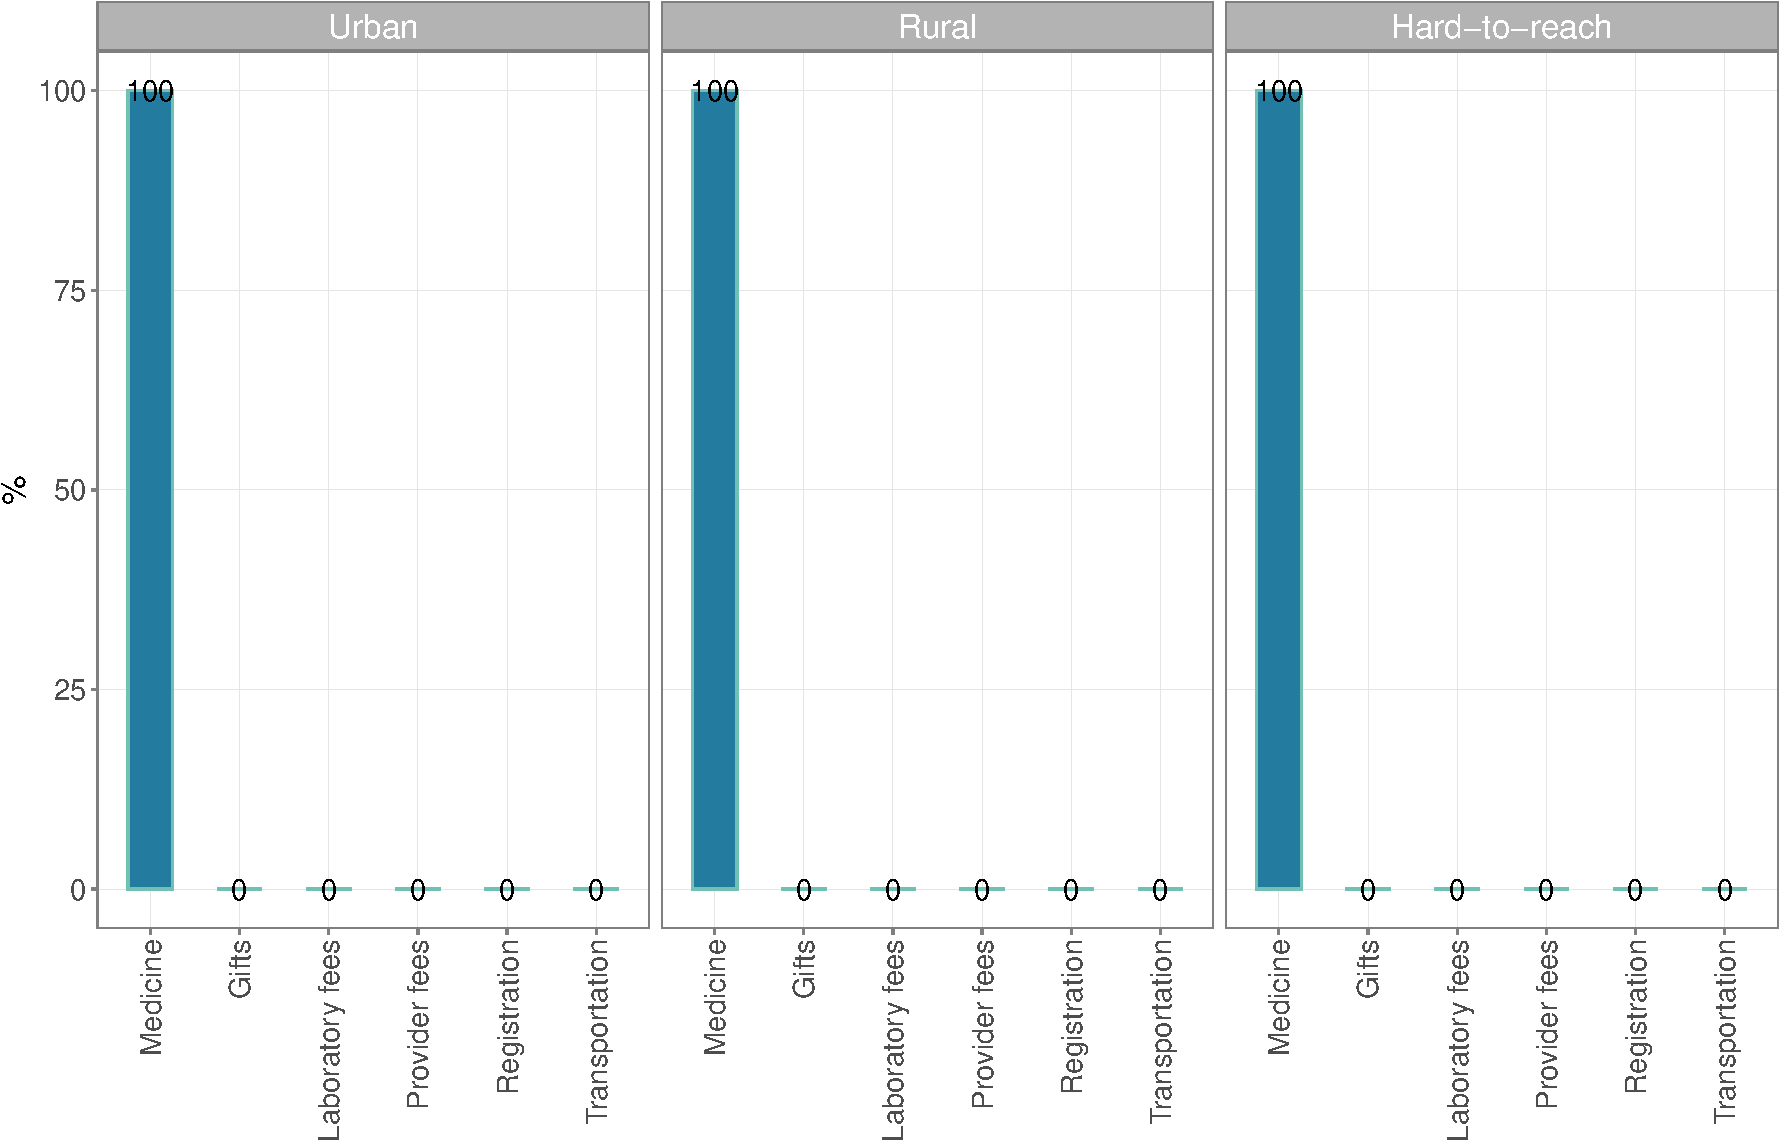
\includegraphics{kayahReport_files/figure-latex/diarrhoea8plot-1} 

}

\caption{Costs incurred for treatment}\label{fig:diarrhoea8plot}
\end{figure}

\hypertarget{ari}{%
\paragraph{Acute respiratory infection}\label{ari}}

\begin{landscape}\begin{table}[H]

\caption{\label{tab:ari1table}Treatment-seeking for acute respiratory infection}
\centering
\fontsize{10}{12}\selectfont
\begin{tabular}[t]{>{\bfseries}l>{\bfseries}l>{\ttfamily}r>{\ttfamily}r>{\ttfamily}r>{\ttfamily}r>{\ttfamily}r>{\ttfamily}r>{\ttfamily}r>{\ttfamily}r>{\ttfamily}r}
\toprule
\multicolumn{4}{c}{\textbf{ }} & \multicolumn{7}{c}{\textbf{Reasons for not seeking treatment}} \\
\cmidrule(l{3pt}r{3pt}){5-11}
 &  & \makecell[c]{Sought\\treatment\\(\%)} & \makecell[c]{Time to\\treatment\\(days)} & \makecell[c]{No\\facility\\(\%)} & \makecell[c]{Facility\\inaccessible\\(\%)} & \makecell[c]{Expensive\\(\%)} & \makecell[c]{Not\\necessary\\(\%)} & \makecell[c]{Advised\\not to\\(\%)} & \makecell[c]{Alternative\\treatment\\(\%)} & \makecell[c]{Do not know\\treamtent\\(\%)}\\
\midrule
\addlinespace[0.3em]
\multicolumn{11}{l}{\textbf{Kayah}}\\
\addlinespace[0.3em]
\multicolumn{11}{l}{\textit{\textbf{Geographic}}}\\
\hspace{1em}\hspace{1em} & Rural & 89.2 & 1.4 & 0.0 & 11.1 & 0.0 & 0.0 & 0 & 11.1 & 0.0\\
\cmidrule{2-11}
\hspace{1em}\hspace{1em} & Urban & 85.0 & 1.3 & 0.0 & 0.0 & 0.0 & 30.0 & 0 & 30.0 & 0.0\\
\cmidrule{2-11}
\hspace{1em}\hspace{1em} & Hard-to-reach & 74.4 & 1.4 & 7.1 & 7.1 & 7.1 & 0.0 & 0 & 0.0 & 21.4\\
\cmidrule{2-11}
\addlinespace[0.3em]
\multicolumn{11}{l}{\textit{\textbf{Wealth}}}\\
\hspace{1em}\hspace{1em} & Wealthiest & 90.9 & 1.3 & 0.0 & 0.0 & 0.0 & 0.0 & 0 & 50.0 & 0.0\\
\cmidrule{2-11}
\hspace{1em}\hspace{1em} & Wealthy & 95.2 & 1.3 & 0.0 & 0.0 & 0.0 & 50.0 & 0 & 0.0 & 0.0\\
\cmidrule{2-11}
\hspace{1em}\hspace{1em} & Medium & 82.6 & 1.2 & 0.0 & 40.0 & 0.0 & 0.0 & 0 & 0.0 & 20.0\\
\cmidrule{2-11}
\hspace{1em}\hspace{1em} & Poor & 75.0 & 1.3 & 10.0 & 0.0 & 0.0 & 0.0 & 0 & 10.0 & 10.0\\
\cmidrule{2-11}
\hspace{1em}\hspace{1em} & Poorest & 73.9 & 1.8 & 0.0 & 0.0 & 9.1 & 18.2 & 0 & 0.0 & 9.1\\
\bottomrule
\end{tabular}
\end{table}
\end{landscape}

\begin{figure}[H]

{\centering 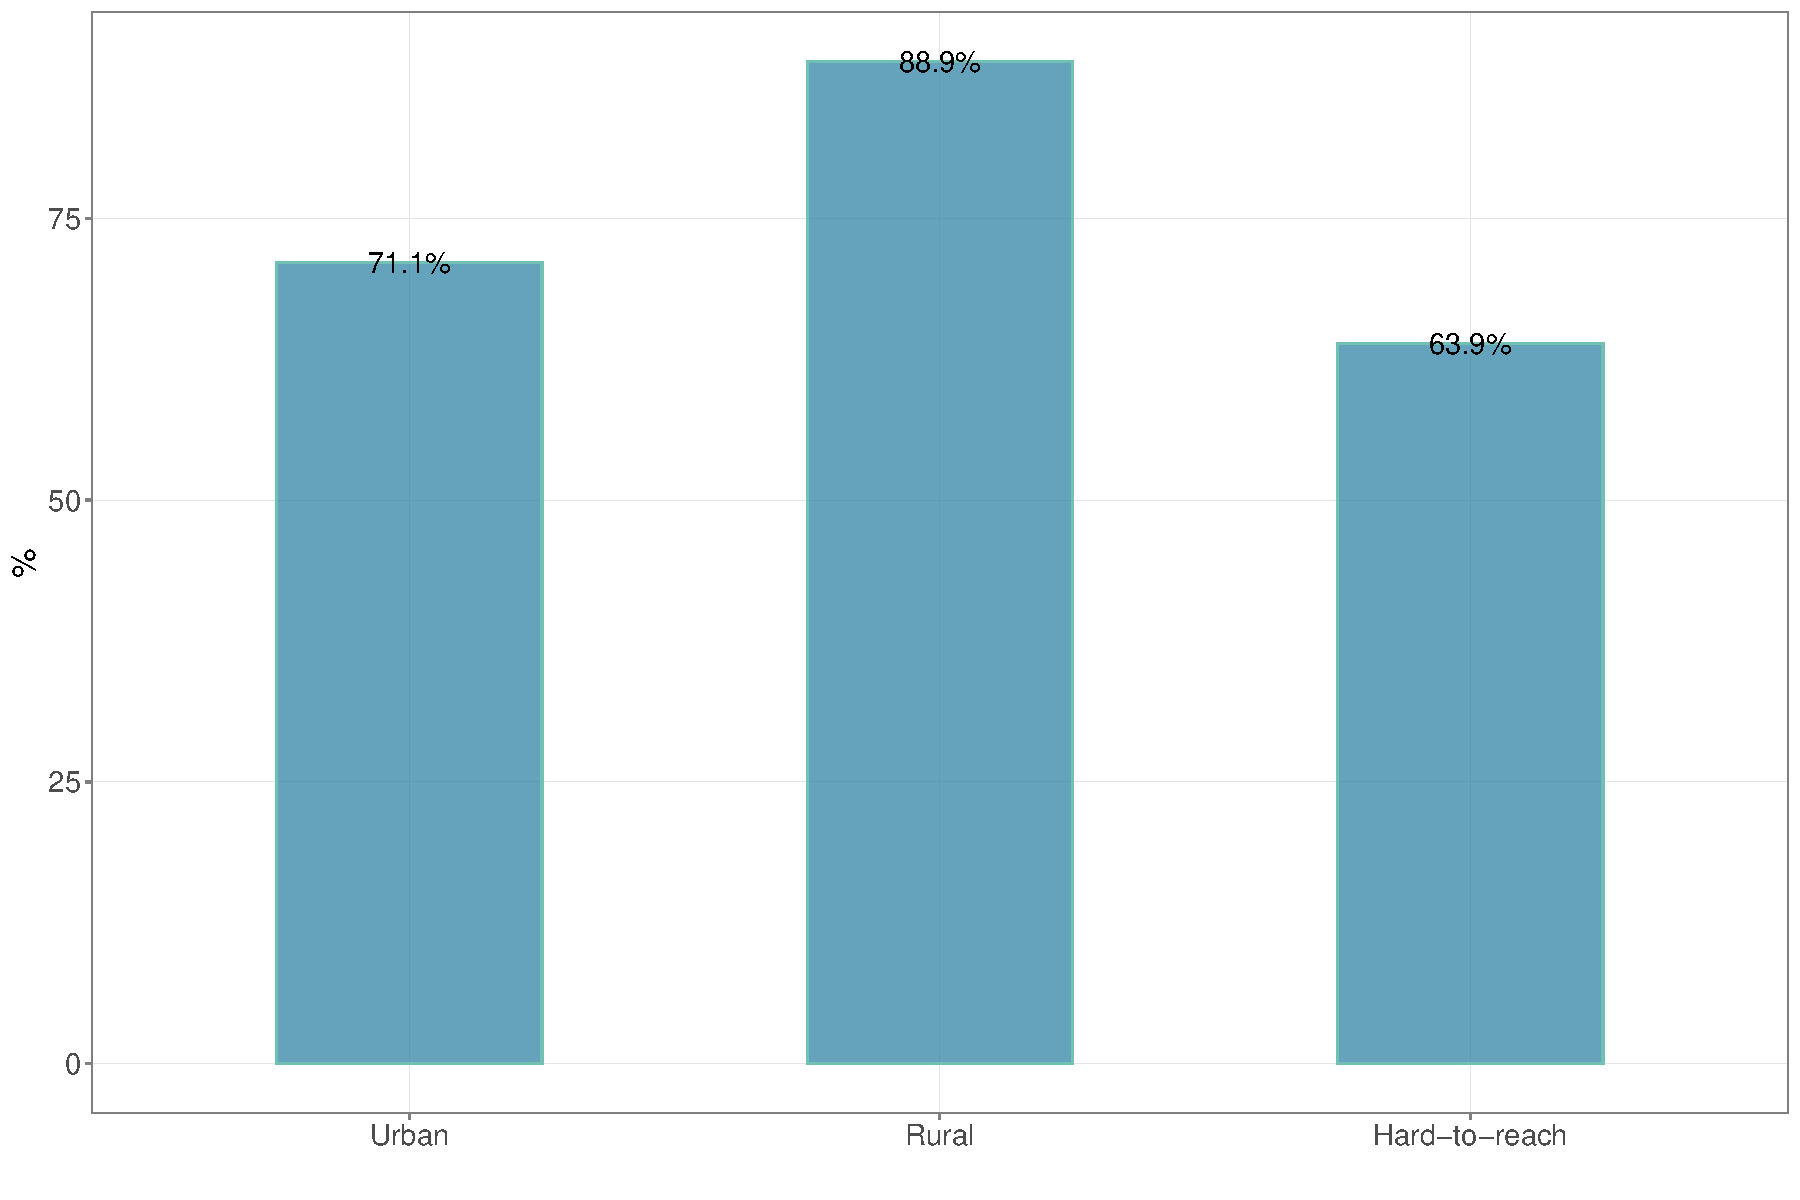
\includegraphics{kayahReport_files/figure-latex/ari1plot-1} 

}

\caption{Treatment-seeking for acute respiratory infection by location type}\label{fig:ari1plot}
\end{figure}

\begin{figure}[H]

{\centering 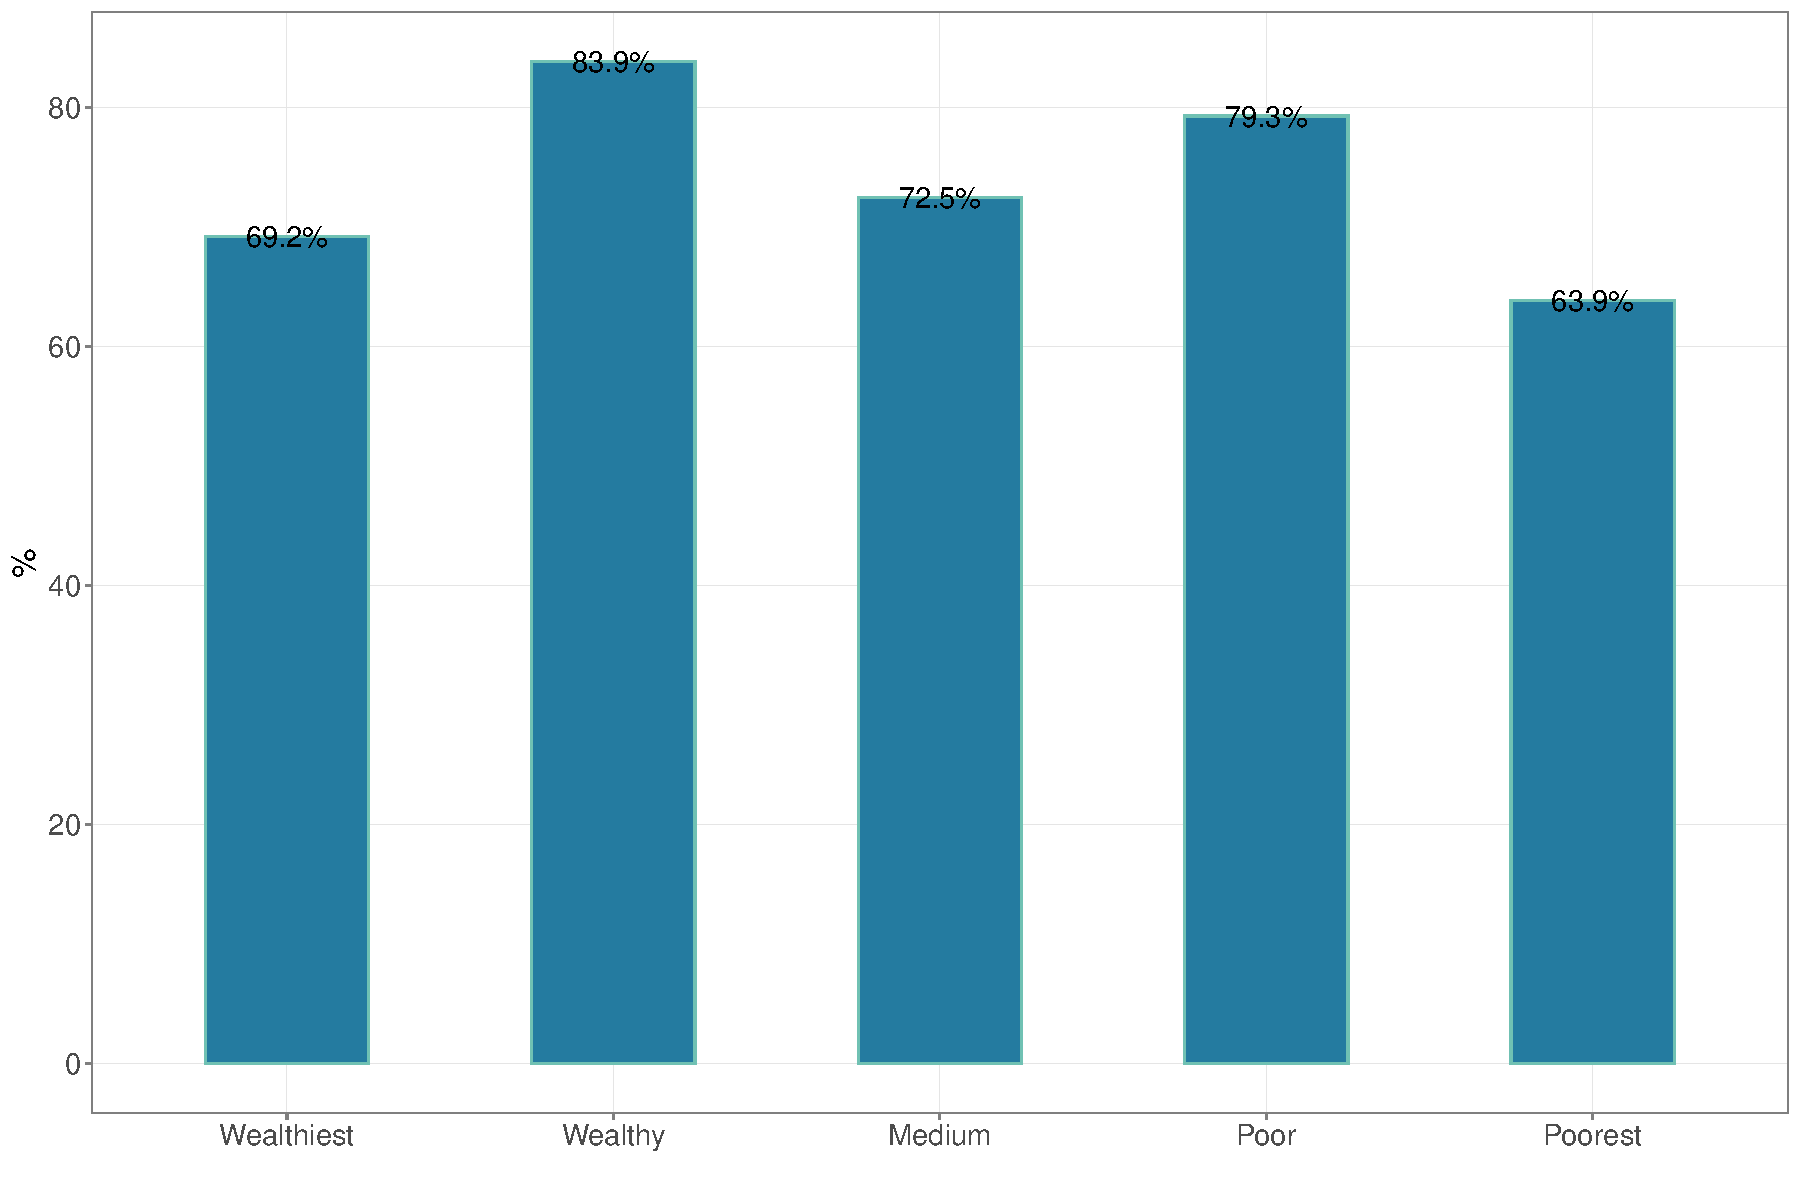
\includegraphics{kayahReport_files/figure-latex/ari2plot-1} 

}

\caption{Treatment-seeking for acute respiratory infection by wealth quintiles}\label{fig:ari2plot}
\end{figure}

\begin{figure}[H]

{\centering 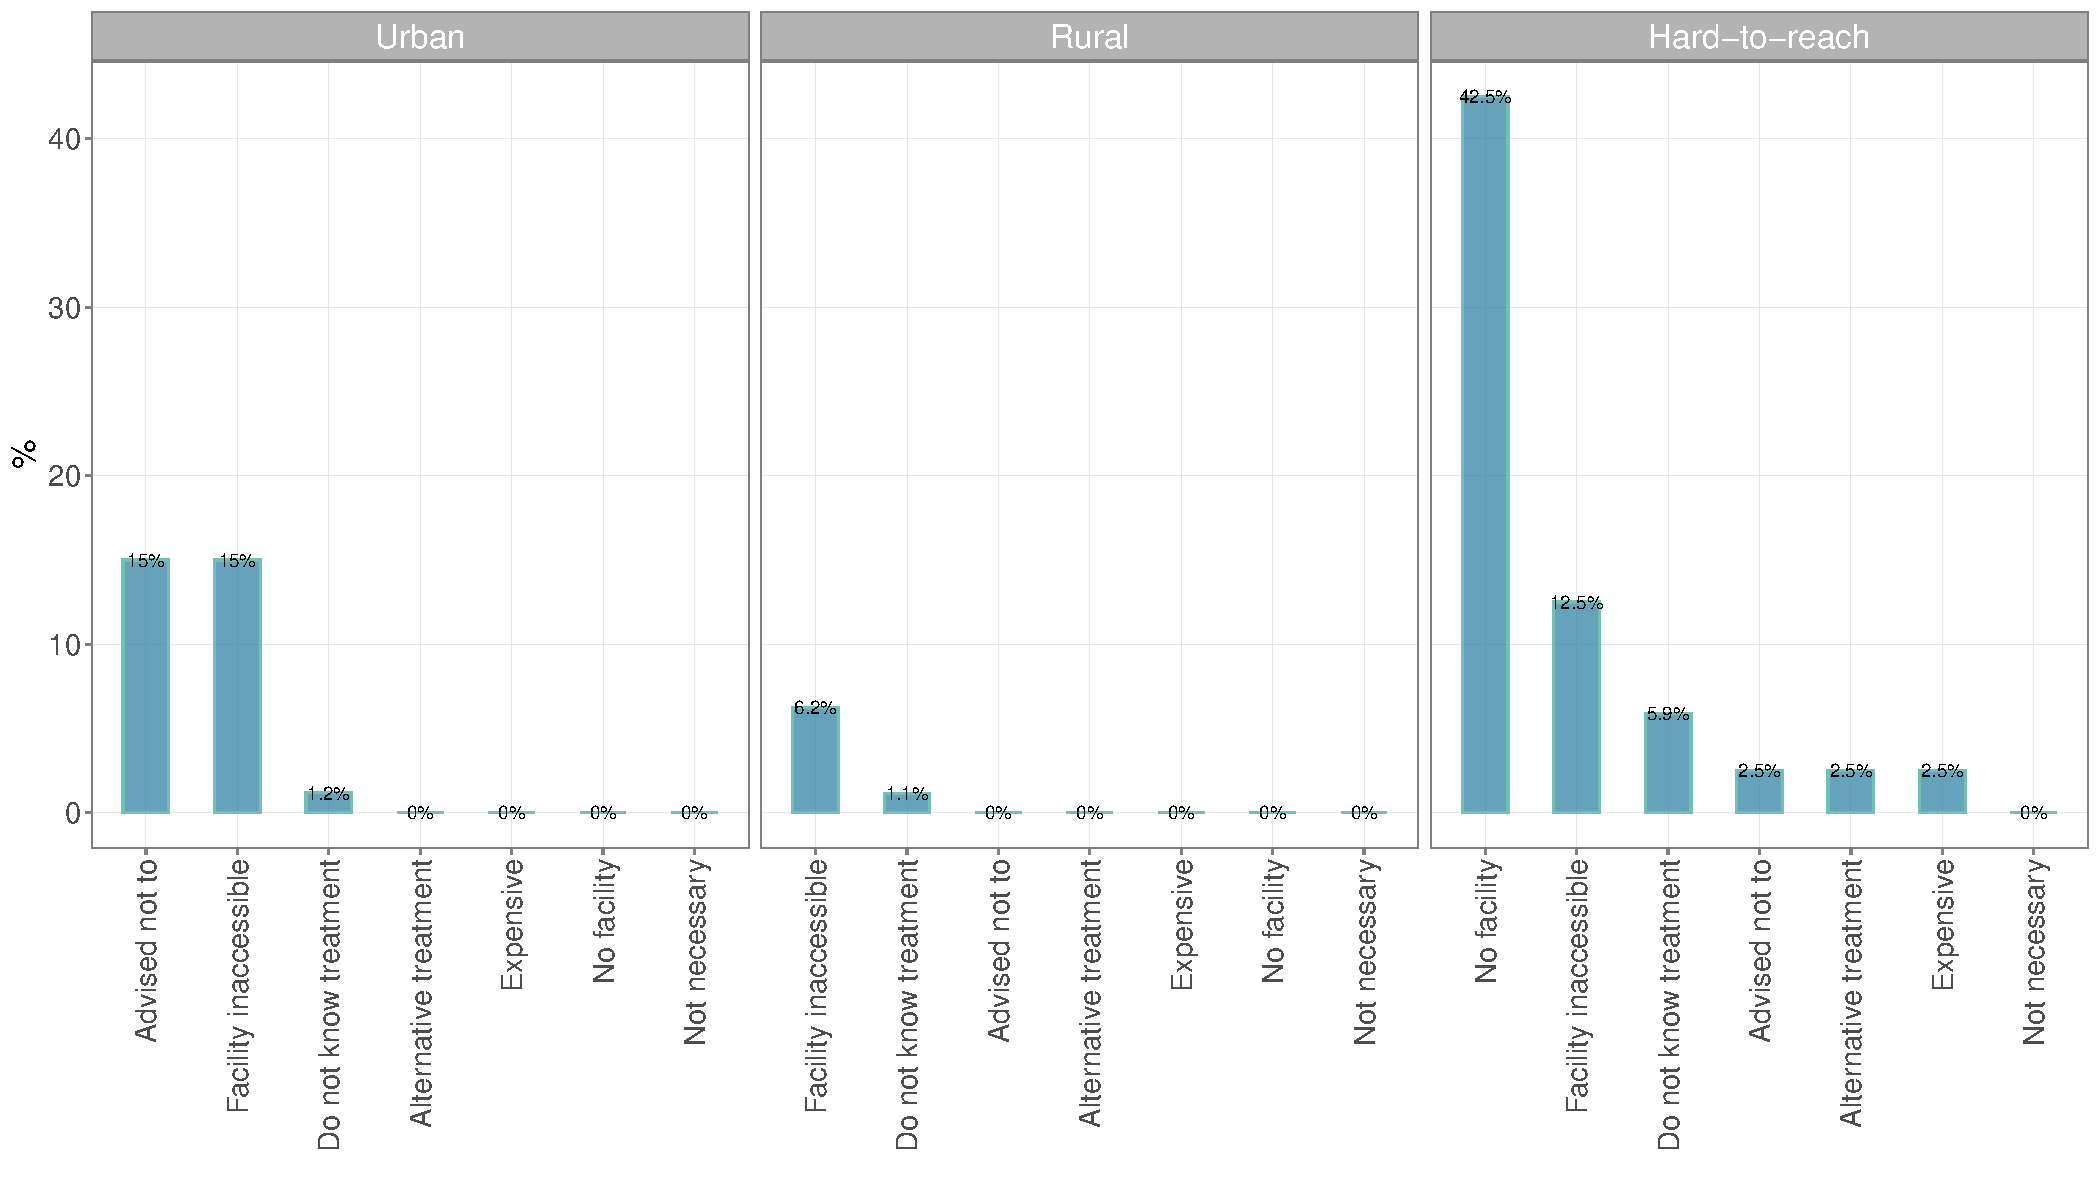
\includegraphics{kayahReport_files/figure-latex/ari4plot-1} 

}

\caption{Reasons for not seeking treatment by location type}\label{fig:ari4plot}
\end{figure}

\begin{landscape}\begin{table}[H]

\caption{\label{tab:ari2table}Where/who treatment is sought from}
\centering
\fontsize{9}{11}\selectfont
\begin{tabular}[t]{>{\bfseries}l>{\bfseries}l>{\ttfamily}r>{\ttfamily}r>{\ttfamily}r>{\ttfamily}r>{\ttfamily}r>{\ttfamily}r>{\ttfamily}r>{\ttfamily}r>{\ttfamily}r>{\ttfamily}r>{\ttfamily}r>{\ttfamily}r>{\ttfamily}r}
\toprule
\multicolumn{2}{c}{\textbf{ }} & \multicolumn{13}{c}{\textbf{Where/who treatment is sought from}} \\
\cmidrule(l{3pt}r{3pt}){3-15}
 &  & \makecell[c]{Township\\hospital\\(\%)} & \makecell[c]{Station\\hospital\\(\%)} & \makecell[c]{RHC/\\health\\assistant\\(\%)} & \makecell[c]{SRHC/\\midwife\\(\%)} & \makecell[c]{Private\\clinic/\\doctor\\(\%)} & \makecell[c]{Community\\health\\worker\\(\%)} & \makecell[c]{Traditional\\healer\\(\%)} & \makecell[c]{Untrained\\health\\worker\\(\%)} & \makecell[c]{Drug\\from\\shop\\(\%)} & \makecell[c]{EHO\\clinic/\\volunteer\\(\%)} & \makecell[c]{Family\\member\\(\%)} & \makecell[c]{NGOs/\\clinic\\(\%)} & \makecell[c]{Auxilliary\\midwife\\(\%)}\\
\midrule
\addlinespace[0.3em]
\multicolumn{15}{l}{\textbf{Kayah}}\\
\addlinespace[0.3em]
\multicolumn{15}{l}{\textit{\textbf{Geographic}}}\\
\hspace{1em}\hspace{1em} & Rural & 1.7 & 8.3 & 18.3 & 18.3 & 21.7 & 5.0 & 0.0 & 0 & 18.3 & 0.0 & 0.0 & 0 & 5.0\\
\cmidrule{2-15}
\hspace{1em}\hspace{1em} & Urban & 3.8 & 0.0 & 1.9 & 0.0 & 73.1 & 0.0 & 0.0 & 0 & 1.9 & 1.9 & 0.0 & 0 & 0.0\\
\cmidrule{2-15}
\hspace{1em}\hspace{1em} & Hard-to-reach & 1.3 & 8.0 & 0.0 & 2.7 & 10.7 & 10.7 & 2.7 & 0 & 25.3 & 26.7 & 2.7 & 0 & 1.3\\
\cmidrule{2-15}
\addlinespace[0.3em]
\multicolumn{15}{l}{\textit{\textbf{Wealth}}}\\
\hspace{1em}\hspace{1em} & Wealthiest & 3.6 & 0.0 & 3.6 & 0.0 & 57.1 & 0.0 & 0.0 & 0 & 3.6 & 3.6 & 0.0 & 0 & 0.0\\
\cmidrule{2-15}
\hspace{1em}\hspace{1em} & Wealthy & 2.4 & 9.5 & 9.5 & 2.4 & 42.9 & 2.4 & 2.4 & 0 & 7.1 & 2.4 & 4.8 & 0 & 2.4\\
\cmidrule{2-15}
\hspace{1em}\hspace{1em} & Medium & 0.0 & 7.3 & 7.3 & 9.8 & 31.7 & 9.8 & 0.0 & 0 & 17.1 & 9.8 & 0.0 & 0 & 0.0\\
\cmidrule{2-15}
\hspace{1em}\hspace{1em} & Poor & 2.4 & 4.9 & 7.3 & 9.8 & 9.8 & 9.8 & 0.0 & 0 & 34.1 & 12.2 & 0.0 & 0 & 7.3\\
\cmidrule{2-15}
\hspace{1em}\hspace{1em} & Poorest & 3.0 & 6.1 & 3.0 & 12.1 & 18.2 & 6.1 & 3.0 & 0 & 18.2 & 30.3 & 0.0 & 0 & 0.0\\
\bottomrule
\end{tabular}
\end{table}
\end{landscape}

\begin{figure}[H]

{\centering 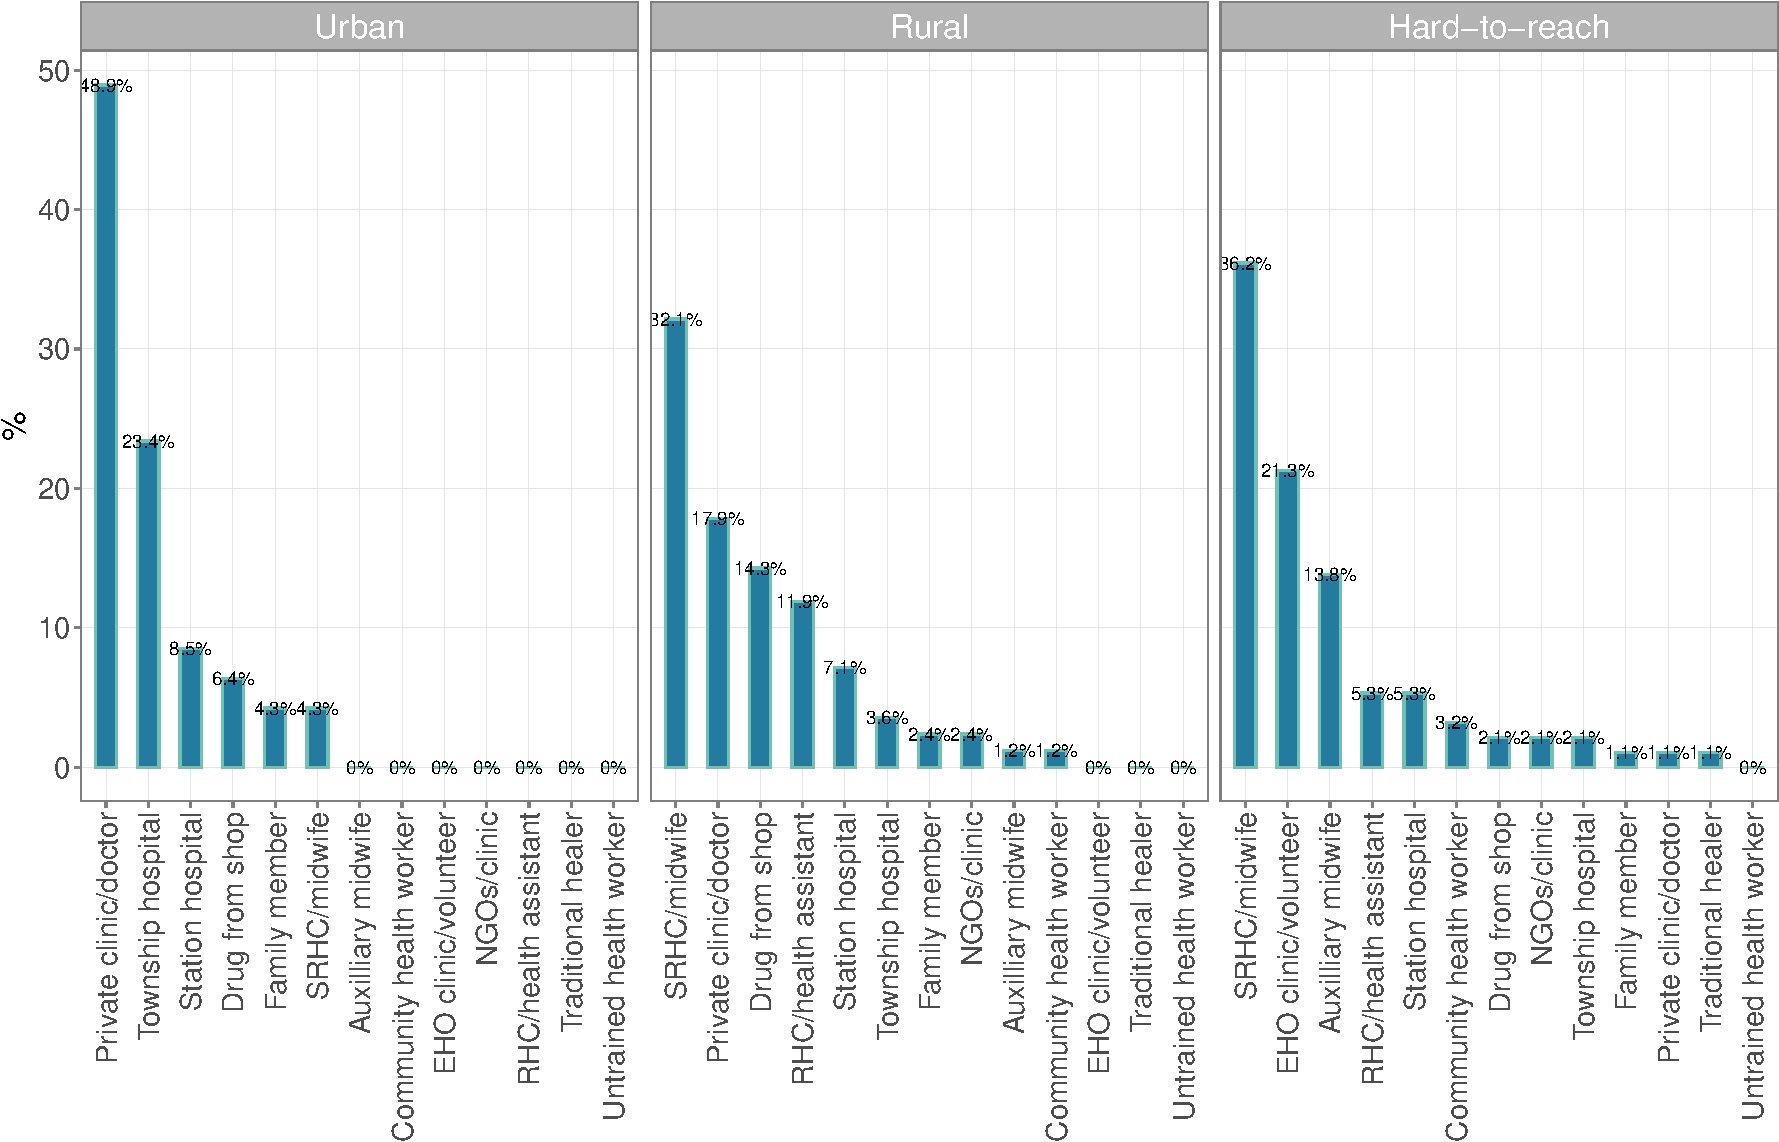
\includegraphics{kayahReport_files/figure-latex/ari6plot-1} 

}

\caption{Where/who treatment is sought from by location type}\label{fig:ari6plot}
\end{figure}

\begin{landscape}\begin{table}[H]

\caption{\label{tab:ari3table}Payment for treatment}
\centering
\fontsize{10}{12}\selectfont
\begin{tabular}[t]{>{\bfseries}l>{\bfseries}l>{\ttfamily}r>{\ttfamily}r>{\ttfamily}r>{\ttfamily}r>{\ttfamily}r>{\ttfamily}r>{\ttfamily}r>{\ttfamily}r}
\toprule
\multicolumn{3}{c}{\textbf{ }} & \multicolumn{6}{c}{\textbf{Payment for}} & \multicolumn{1}{c}{\textbf{ }} \\
\cmidrule(l{3pt}r{3pt}){4-9}
 &  & \makecell[c]{Payment\\for\\service\\(MMK)} & \makecell[c]{Transportation\\(\%)} & \makecell[c]{Registration\\(\%)} & \makecell[c]{Medicine\\(\%)} & \makecell[c]{Laboratory\\fees\\(\%)} & \makecell[c]{Provider\\fees\\(\%)} & \makecell[c]{Gifts\\(\%)} & \makecell[c]{Took\\loan\\(\%)}\\
\midrule
\addlinespace[0.3em]
\multicolumn{10}{l}{\textbf{Kayah}}\\
\addlinespace[0.3em]
\multicolumn{10}{l}{\textit{\textbf{Geographic}}}\\
\hspace{1em}\hspace{1em} & Rural & 7076.7 & 0.0 & 0.0 & 100.0 & 0 & 0 & 0 & 3.8\\
\cmidrule{2-10}
\hspace{1em}\hspace{1em} & Urban & 12028.8 & 0.0 & 0.0 & 100.0 & 0 & 0 & 0 & 6.0\\
\cmidrule{2-10}
\hspace{1em}\hspace{1em} & Hard-to-reach & 5360.0 & 2.6 & 2.6 & 92.3 & 0 & 0 & 0 & 11.1\\
\cmidrule{2-10}
\addlinespace[0.3em]
\multicolumn{10}{l}{\textit{\textbf{Wealth}}}\\
\hspace{1em}\hspace{1em} & Wealthiest & 13196.4 & 0.0 & 0.0 & 100.0 & 0 & 0 & 0 & 3.8\\
\cmidrule{2-10}
\hspace{1em}\hspace{1em} & Wealthy & 9154.8 & 0.0 & 0.0 & 100.0 & 0 & 0 & 0 & 2.5\\
\cmidrule{2-10}
\hspace{1em}\hspace{1em} & Medium & 8739.0 & 0.0 & 0.0 & 95.7 & 0 & 0 & 0 & 5.9\\
\cmidrule{2-10}
\hspace{1em}\hspace{1em} & Poor & 3982.9 & 0.0 & 0.0 & 100.0 & 0 & 0 & 0 & 14.7\\
\cmidrule{2-10}
\hspace{1em}\hspace{1em} & Poorest & 4590.9 & 6.7 & 6.7 & 86.7 & 0 & 0 & 0 & 9.5\\
\bottomrule
\end{tabular}
\end{table}
\end{landscape}

\begin{figure}[H]

{\centering 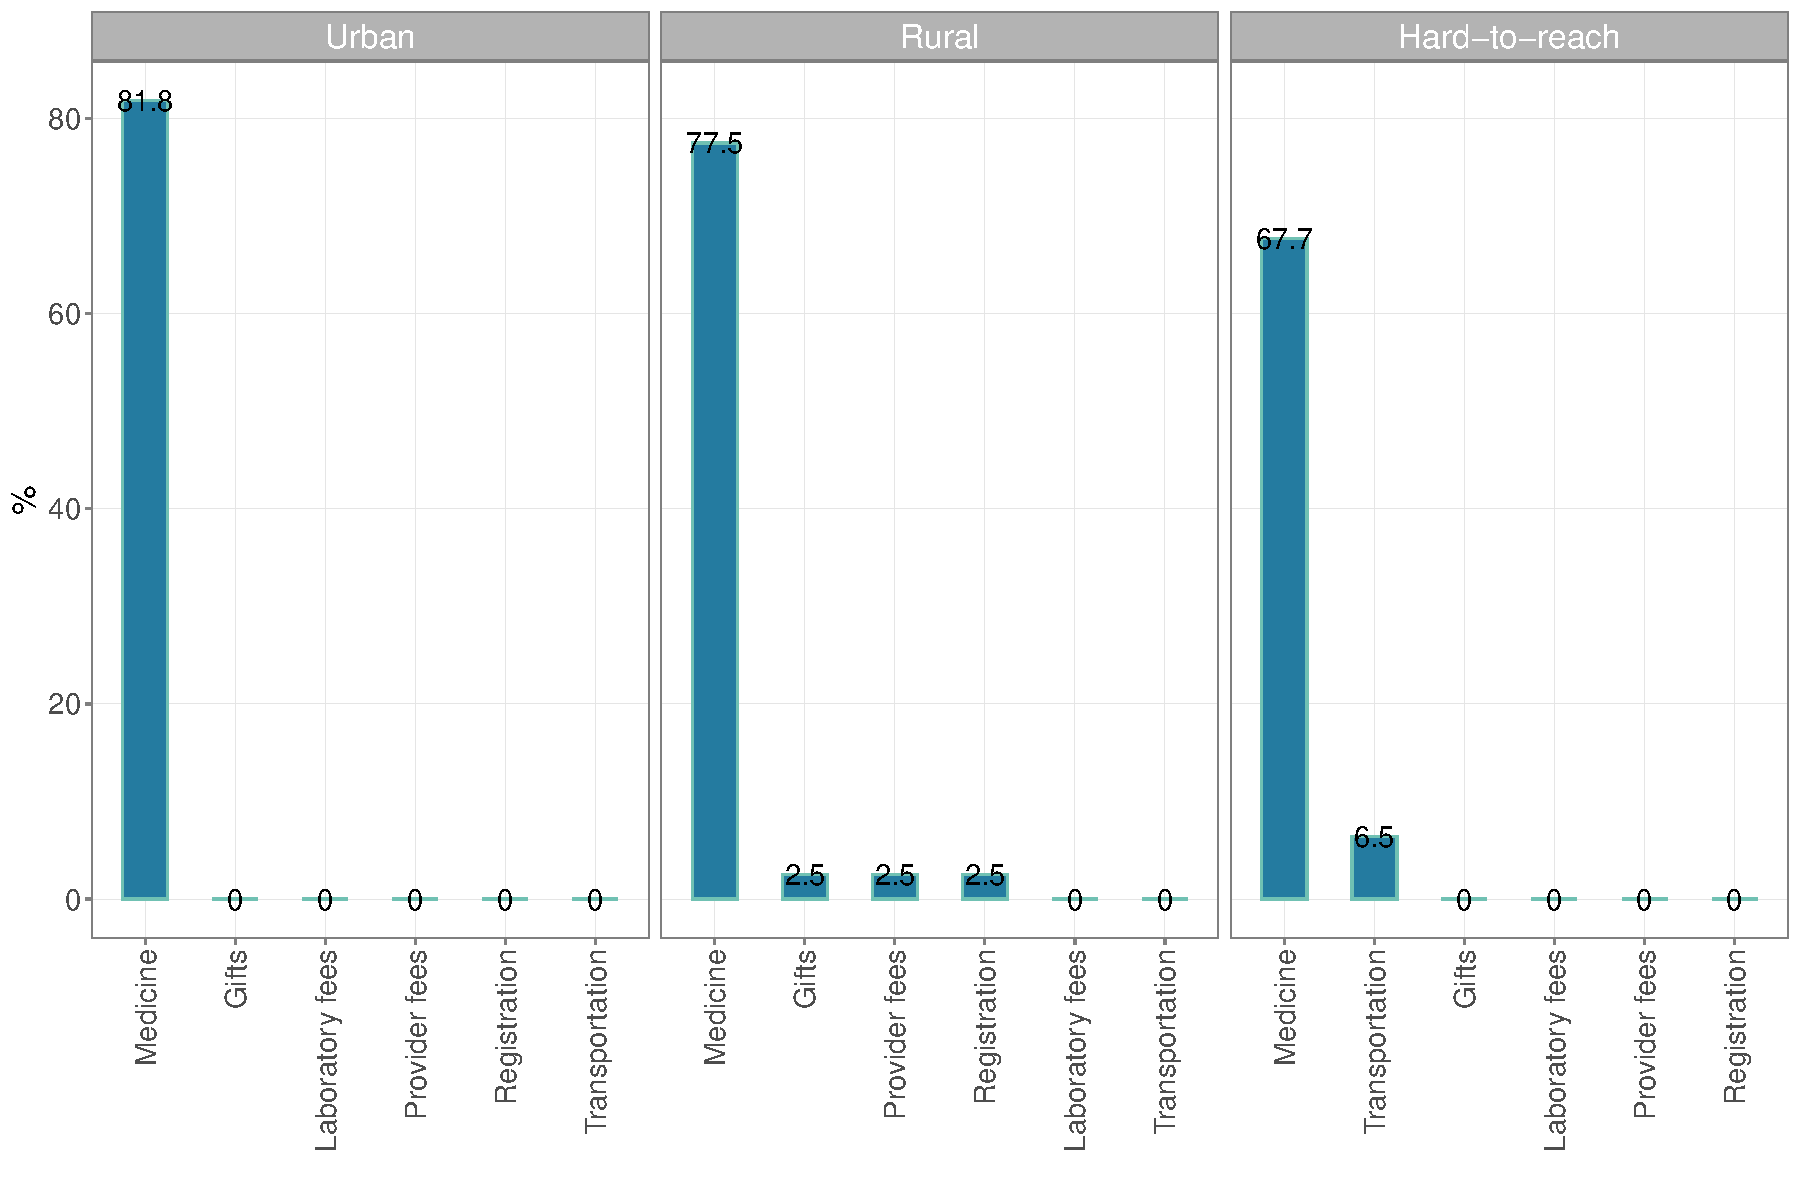
\includegraphics{kayahReport_files/figure-latex/ari8plot-1} 

}

\caption{Costs incurred for treatment by location type}\label{fig:ari8plot}
\end{figure}

\hypertarget{fever}{%
\paragraph{Fever}\label{fever}}

\begin{landscape}\begin{table}[H]

\caption{\label{tab:fever1table}Treatment-seeking for fever}
\centering
\fontsize{10}{12}\selectfont
\begin{tabular}[t]{>{\bfseries}l>{\bfseries}l>{\ttfamily}r>{\ttfamily}r>{\ttfamily}r>{\ttfamily}r>{\ttfamily}r>{\ttfamily}r>{\ttfamily}r>{\ttfamily}r>{\ttfamily}r}
\toprule
\multicolumn{4}{c}{\textbf{ }} & \multicolumn{7}{c}{\textbf{Reasons for not seeking treatment}} \\
\cmidrule(l{3pt}r{3pt}){5-11}
 &  & \makecell[c]{Sought\\treatment\\(\%)} & \makecell[c]{Time to\\treatment\\(days)} & \makecell[c]{No\\facility\\(\%)} & \makecell[c]{Facility\\inaccessible\\(\%)} & \makecell[c]{Expensive\\(\%)} & \makecell[c]{Not\\necessary\\(\%)} & \makecell[c]{Advised\\not to\\(\%)} & \makecell[c]{Alternative\\treatment\\(\%)} & \makecell[c]{Do not know\\treamtent\\(\%)}\\
\midrule
\addlinespace[0.3em]
\multicolumn{11}{l}{\textbf{Kayah}}\\
\addlinespace[0.3em]
\multicolumn{11}{l}{\textit{\textbf{Geographic}}}\\
\hspace{1em}\hspace{1em} & Rural & 94.0 & 1.1 & 0.0 & 0.0 & 8.3 & 8.3 & 0 & 25.0 & 0.0\\
\cmidrule{2-11}
\hspace{1em}\hspace{1em} & Urban & 91.3 & 1.2 & 0.0 & 0.0 & 0.0 & 18.8 & 0 & 18.8 & 0.0\\
\cmidrule{2-11}
\hspace{1em}\hspace{1em} & Hard-to-reach & 79.0 & 1.4 & 5.0 & 10.0 & 5.0 & 5.0 & 0 & 0.0 & 5.0\\
\cmidrule{2-11}
\addlinespace[0.3em]
\multicolumn{11}{l}{\textit{\textbf{Wealth}}}\\
\hspace{1em}\hspace{1em} & Wealthiest & 91.0 & 1.1 & 0.0 & 0.0 & 0.0 & 0.0 & 0 & 22.2 & 0.0\\
\cmidrule{2-11}
\hspace{1em}\hspace{1em} & Wealthy & 90.3 & 1.3 & 0.0 & 0.0 & 11.1 & 11.1 & 0 & 11.1 & 0.0\\
\cmidrule{2-11}
\hspace{1em}\hspace{1em} & Medium & 92.9 & 1.1 & 0.0 & 0.0 & 0.0 & 14.3 & 0 & 14.3 & 0.0\\
\cmidrule{2-11}
\hspace{1em}\hspace{1em} & Poor & 92.9 & 1.2 & 0.0 & 0.0 & 0.0 & 0.0 & 0 & 28.6 & 14.3\\
\cmidrule{2-11}
\hspace{1em}\hspace{1em} & Poorest & 79.2 & 1.5 & 6.2 & 12.5 & 6.2 & 18.8 & 0 & 0.0 & 0.0\\
\bottomrule
\end{tabular}
\end{table}
\end{landscape}

\begin{figure}[H]

{\centering 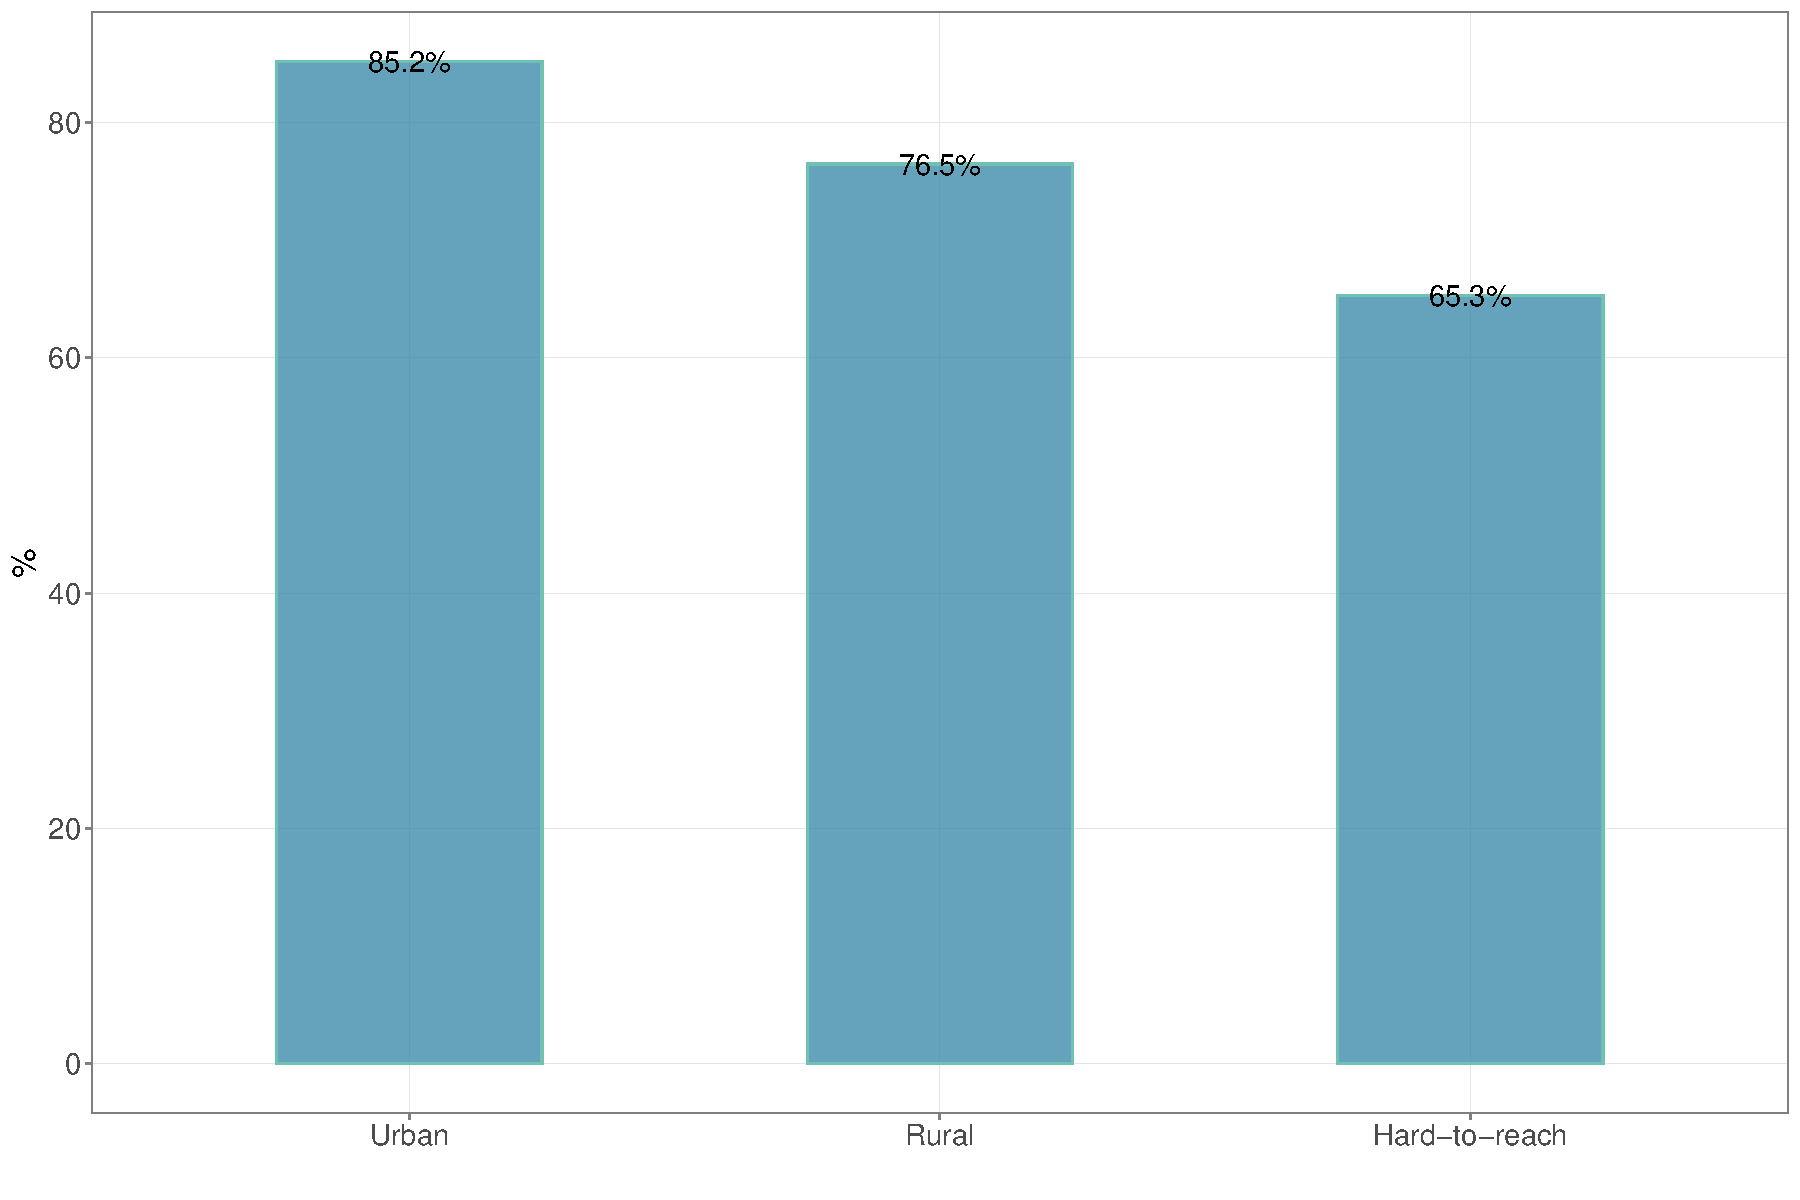
\includegraphics{kayahReport_files/figure-latex/fever1plot-1} 

}

\caption{Treatment-seeking for fever by location type}\label{fig:fever1plot}
\end{figure}

\begin{figure}[H]

{\centering 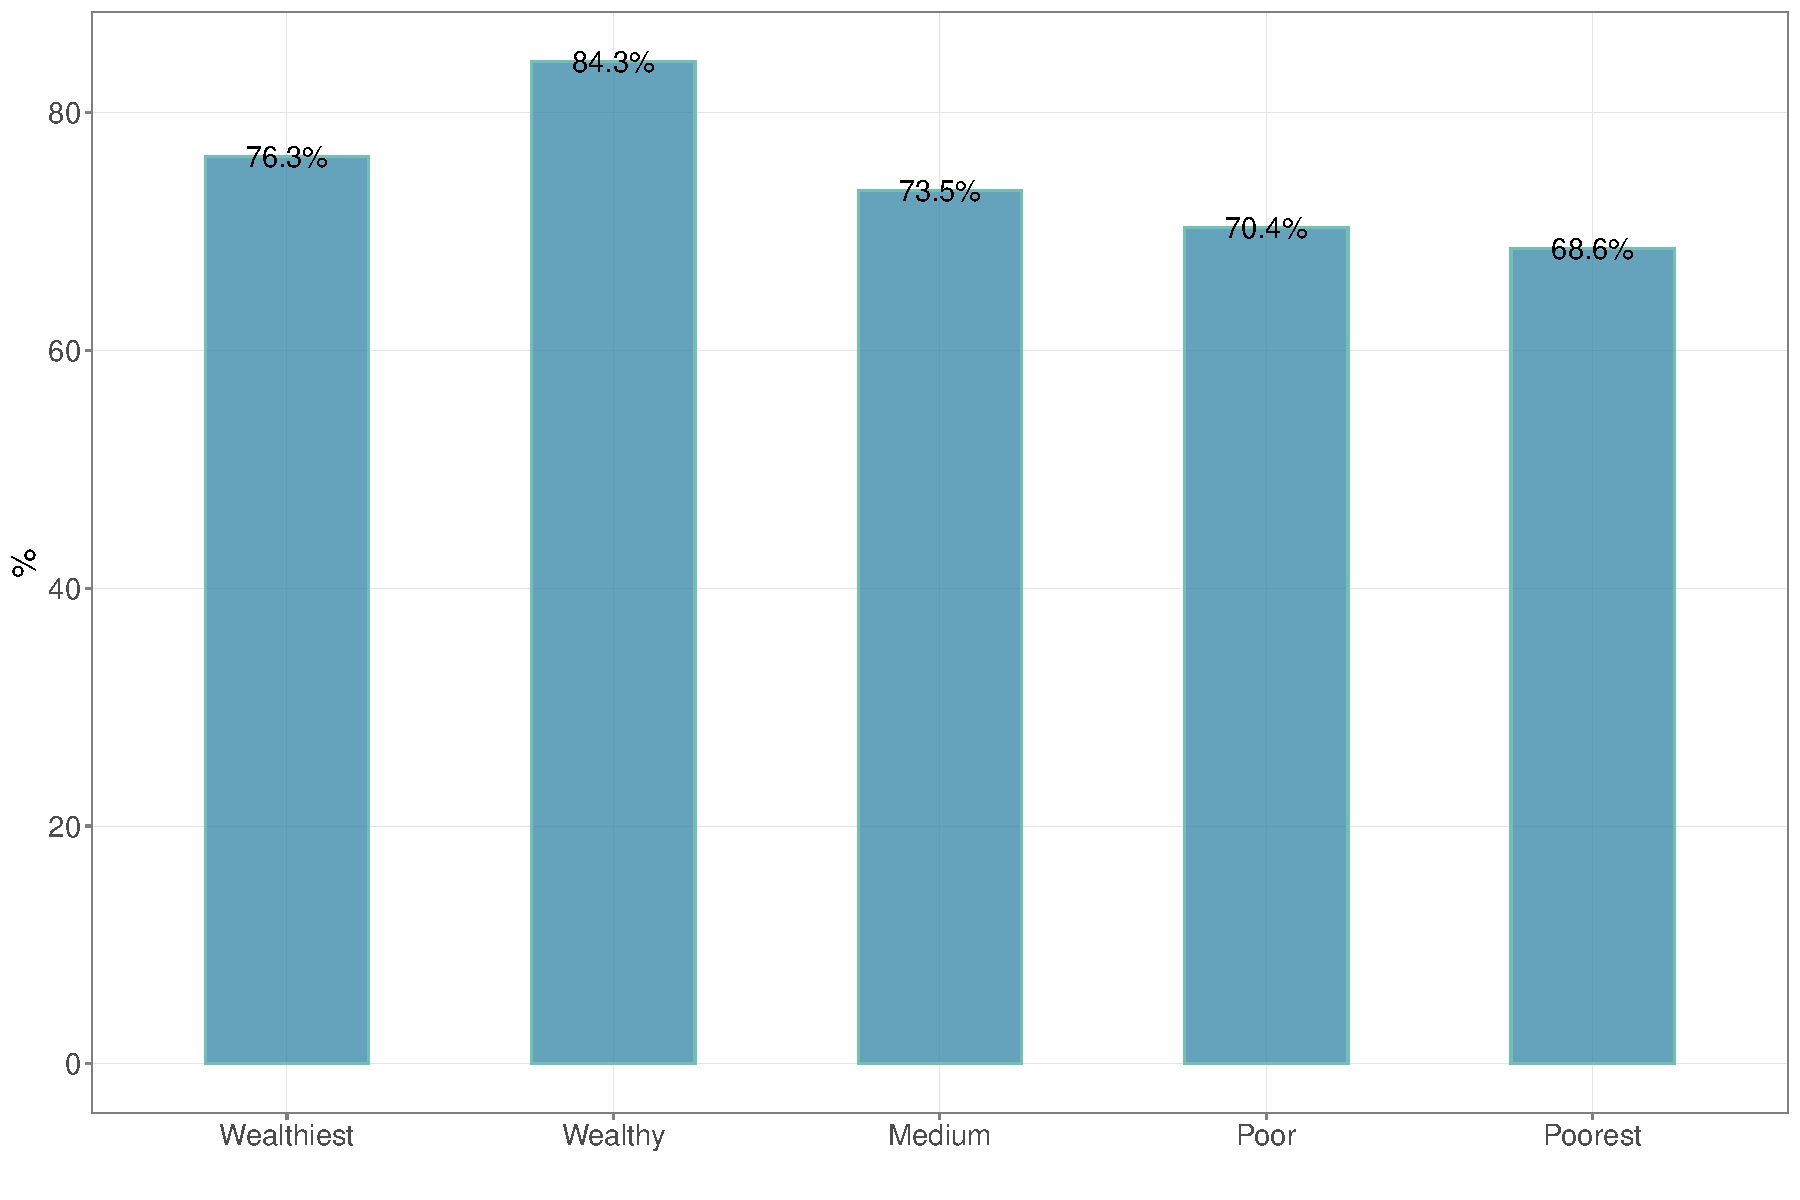
\includegraphics{kayahReport_files/figure-latex/fever2plot-1} 

}

\caption{Treatment-seeking for fever by wealth quintiles}\label{fig:fever2plot}
\end{figure}

\begin{figure}[H]

{\centering 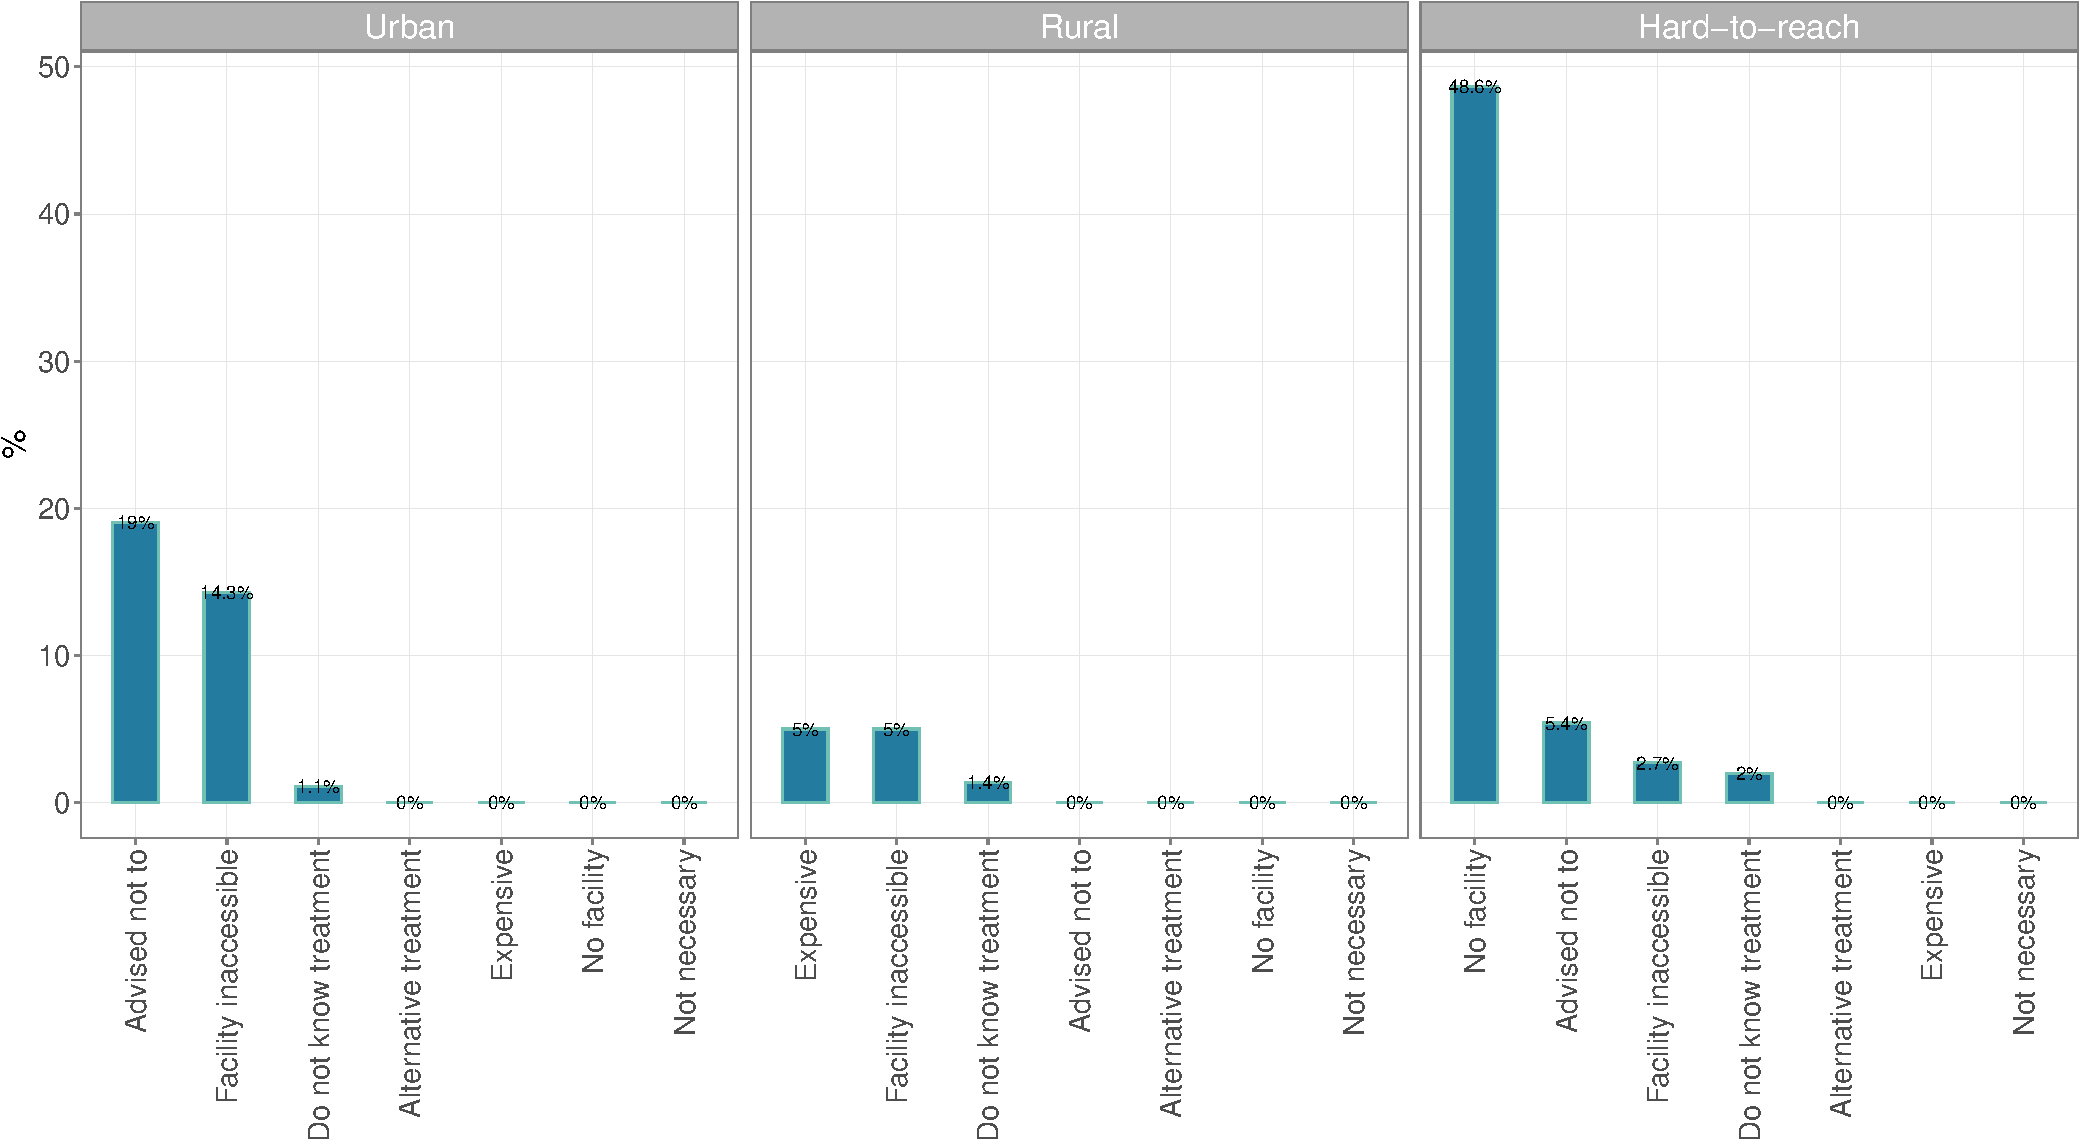
\includegraphics{kayahReport_files/figure-latex/fever4plot-1} 

}

\caption{Reasons for not seeking treatment by location type}\label{fig:fever4plot}
\end{figure}

\begin{landscape}\begin{table}[H]

\caption{\label{tab:fever2table}Where/who treatment is sought from}
\centering
\fontsize{9}{11}\selectfont
\begin{tabular}[t]{>{\bfseries}l>{\bfseries}l>{\ttfamily}r>{\ttfamily}r>{\ttfamily}r>{\ttfamily}r>{\ttfamily}r>{\ttfamily}r>{\ttfamily}r>{\ttfamily}r>{\ttfamily}r>{\ttfamily}r>{\ttfamily}r>{\ttfamily}r>{\ttfamily}r}
\toprule
\multicolumn{2}{c}{\textbf{ }} & \multicolumn{13}{c}{\textbf{Where/who treatment is sought from}} \\
\cmidrule(l{3pt}r{3pt}){3-15}
 &  & \makecell[c]{Township\\hospital\\(\%)} & \makecell[c]{Station\\hospital\\(\%)} & \makecell[c]{RHC/\\health\\assistant\\(\%)} & \makecell[c]{SRHC/\\midwife\\(\%)} & \makecell[c]{Private\\clinic/\\doctor\\(\%)} & \makecell[c]{Community\\health\\worker\\(\%)} & \makecell[c]{Traditional\\healer\\(\%)} & \makecell[c]{Untrained\\health\\worker\\(\%)} & \makecell[c]{Drug\\from\\shop\\(\%)} & \makecell[c]{EHO\\clinic/\\volunteer\\(\%)} & \makecell[c]{Family\\member\\(\%)} & \makecell[c]{NGOs/\\clinic\\(\%)} & \makecell[c]{Auxilliary\\midwife\\(\%)}\\
\midrule
\addlinespace[0.3em]
\multicolumn{15}{l}{\textbf{Kayah}}\\
\addlinespace[0.3em]
\multicolumn{15}{l}{\textit{\textbf{Geographic}}}\\
\hspace{1em}\hspace{1em} & Rural & 3.5 & 5.6 & 17.5 & 25.2 & 17.5 & 2.1 & 0.7 & 2.8 & 12.6 & 0.0 & 2.8 & 0 & 3.5\\
\cmidrule{2-15}
\hspace{1em}\hspace{1em} & Urban & 3.6 & 0.7 & 1.5 & 0.0 & 82.5 & 0.7 & 0.0 & 0.0 & 4.4 & 0.0 & 0.0 & 0 & 0.0\\
\cmidrule{2-15}
\hspace{1em}\hspace{1em} & Hard-to-reach & 2.0 & 7.0 & 1.0 & 7.0 & 11.0 & 9.0 & 1.0 & 1.0 & 22.0 & 29.0 & 2.0 & 0 & 3.0\\
\cmidrule{2-15}
\addlinespace[0.3em]
\multicolumn{15}{l}{\textit{\textbf{Wealth}}}\\
\hspace{1em}\hspace{1em} & Wealthiest & 2.8 & 2.8 & 2.8 & 0.0 & 77.5 & 0.0 & 0.0 & 0.0 & 4.2 & 0.0 & 0.0 & 0 & 0.0\\
\cmidrule{2-15}
\hspace{1em}\hspace{1em} & Wealthy & 3.4 & 5.7 & 6.9 & 8.0 & 54.0 & 1.1 & 0.0 & 1.1 & 5.7 & 3.4 & 3.4 & 0 & 0.0\\
\cmidrule{2-15}
\hspace{1em}\hspace{1em} & Medium & 2.2 & 5.5 & 7.7 & 17.6 & 22.0 & 7.7 & 0.0 & 4.4 & 11.0 & 11.0 & 2.2 & 0 & 2.2\\
\cmidrule{2-15}
\hspace{1em}\hspace{1em} & Poor & 4.5 & 6.1 & 16.7 & 18.2 & 16.7 & 4.5 & 1.5 & 0.0 & 15.2 & 9.1 & 0.0 & 0 & 3.0\\
\cmidrule{2-15}
\hspace{1em}\hspace{1em} & Poorest & 0.0 & 0.0 & 3.5 & 14.0 & 19.3 & 3.5 & 1.8 & 0.0 & 31.6 & 17.5 & 0.0 & 0 & 7.0\\
\bottomrule
\end{tabular}
\end{table}
\end{landscape}

\begin{figure}[H]

{\centering 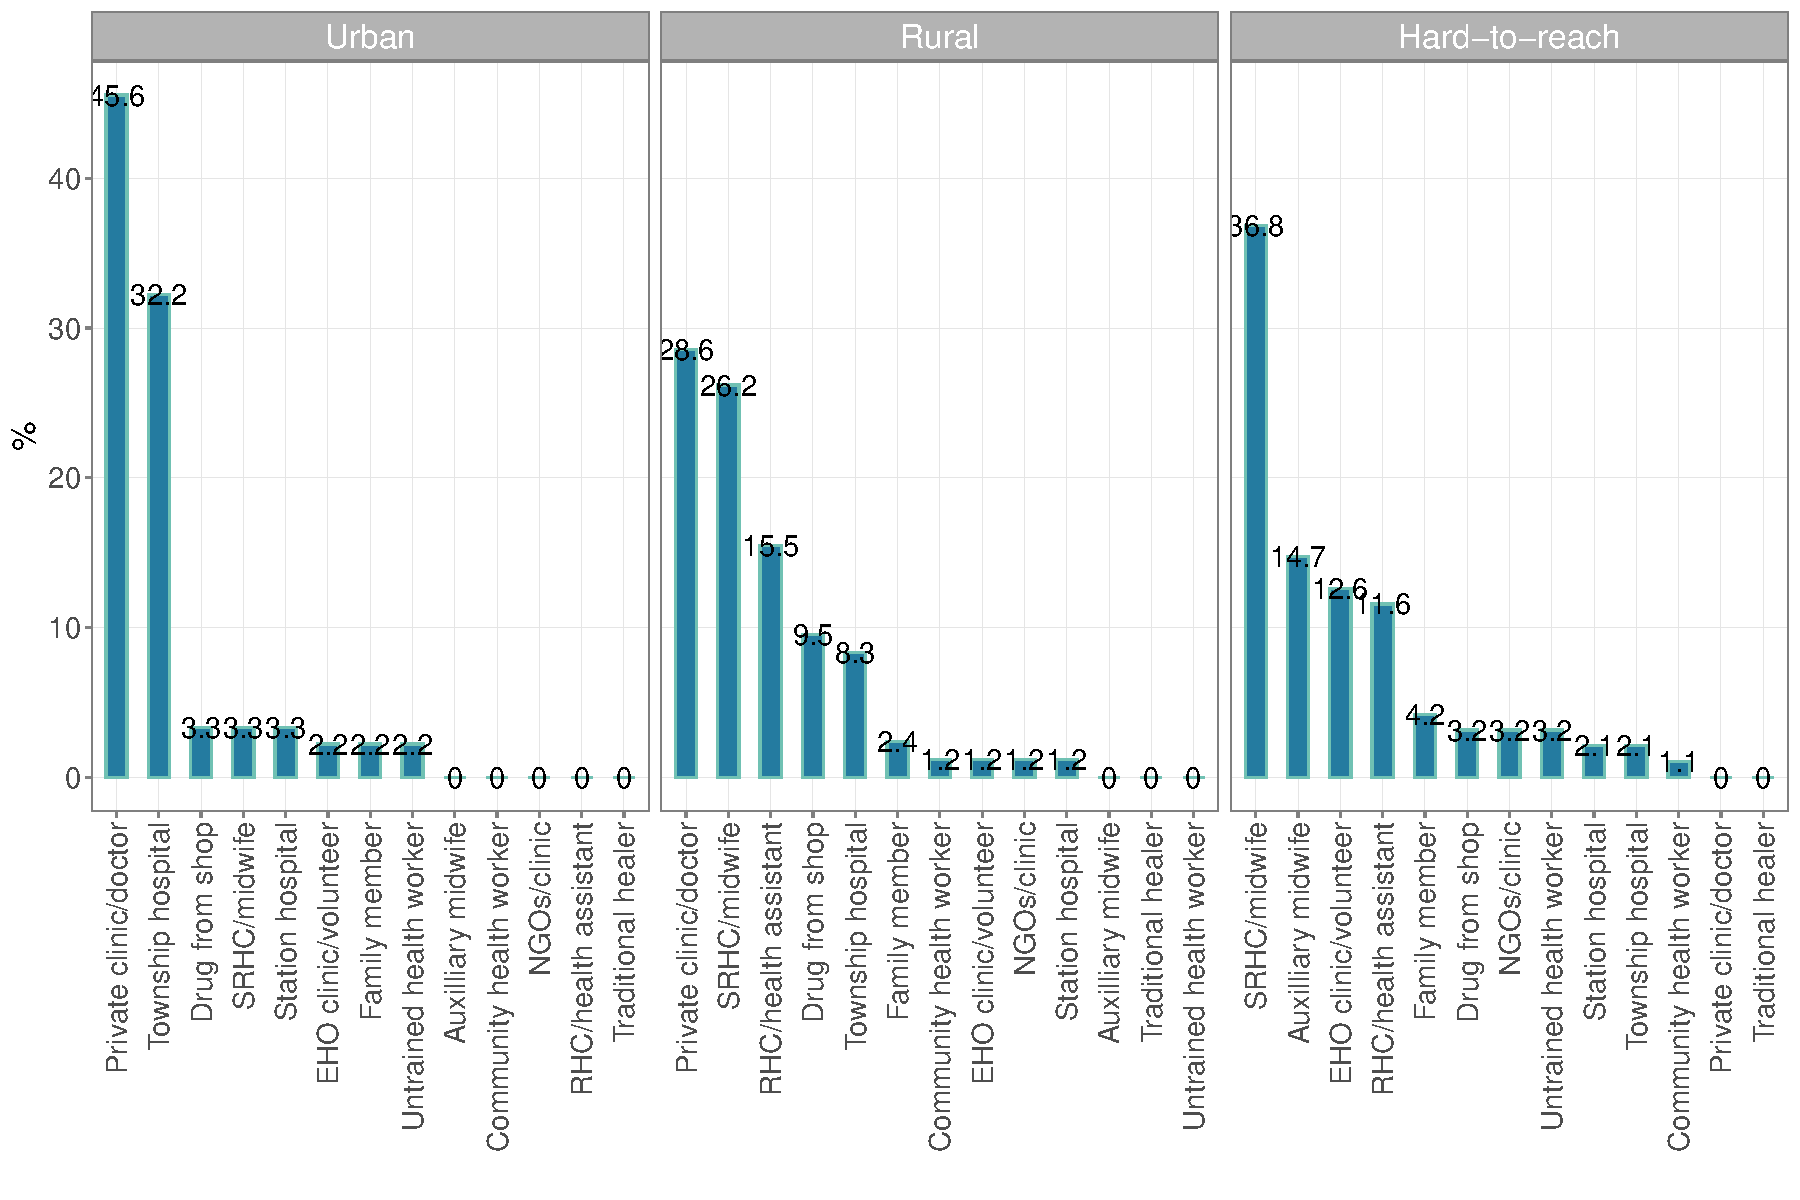
\includegraphics{kayahReport_files/figure-latex/fever6plot-1} 

}

\caption{Where/who treatment is sought from by location type}\label{fig:fever6plot}
\end{figure}

\begin{landscape}\begin{table}[H]

\caption{\label{tab:fever3table}Payment for treatment}
\centering
\fontsize{10}{12}\selectfont
\begin{tabular}[t]{>{\bfseries}l>{\bfseries}l>{\ttfamily}r>{\ttfamily}r>{\ttfamily}r>{\ttfamily}r>{\ttfamily}r>{\ttfamily}r>{\ttfamily}r>{\ttfamily}r}
\toprule
\multicolumn{3}{c}{\textbf{ }} & \multicolumn{6}{c}{\textbf{Payment for}} & \multicolumn{1}{c}{\textbf{ }} \\
\cmidrule(l{3pt}r{3pt}){4-9}
 &  & \makecell[c]{Payment\\for\\service\\(MMK)} & \makecell[c]{Transportation\\(\%)} & \makecell[c]{Registration\\(\%)} & \makecell[c]{Medicine\\(\%)} & \makecell[c]{Laboratory\\fees\\(\%)} & \makecell[c]{Provider\\fees\\(\%)} & \makecell[c]{Gifts\\(\%)} & \makecell[c]{Took\\loan\\(\%)}\\
\midrule
\addlinespace[0.3em]
\multicolumn{10}{l}{\textbf{Kayah}}\\
\addlinespace[0.3em]
\multicolumn{10}{l}{\textit{\textbf{Geographic}}}\\
\hspace{1em}\hspace{1em} & Rural & 13020.5 & 1.2 & 0 & 97.5 & 0 & 0 & 0 & 9.9\\
\cmidrule{2-10}
\hspace{1em}\hspace{1em} & Urban & 13923.4 & 0.0 & 0 & 100.0 & 0 & 0 & 0 & 12.8\\
\cmidrule{2-10}
\hspace{1em}\hspace{1em} & Hard-to-reach & 8271.0 & 5.5 & 0 & 94.5 & 0 & 0 & 0 & 8.5\\
\cmidrule{2-10}
\addlinespace[0.3em]
\multicolumn{10}{l}{\textit{\textbf{Wealth}}}\\
\hspace{1em}\hspace{1em} & Wealthiest & 17457.7 & 0.0 & 0 & 100.0 & 0 & 0 & 0 & 5.7\\
\cmidrule{2-10}
\hspace{1em}\hspace{1em} & Wealthy & 11106.9 & 2.6 & 0 & 94.7 & 0 & 0 & 0 & 6.2\\
\cmidrule{2-10}
\hspace{1em}\hspace{1em} & Medium & 6945.5 & 0.0 & 0 & 100.0 & 0 & 0 & 0 & 10.5\\
\cmidrule{2-10}
\hspace{1em}\hspace{1em} & Poor & 18649.8 & 4.9 & 0 & 95.1 & 0 & 0 & 0 & 19.0\\
\cmidrule{2-10}
\hspace{1em}\hspace{1em} & Poorest & 5154.4 & 3.1 & 0 & 96.9 & 0 & 0 & 0 & 13.6\\
\bottomrule
\end{tabular}
\end{table}
\end{landscape}

\begin{figure}[H]

{\centering 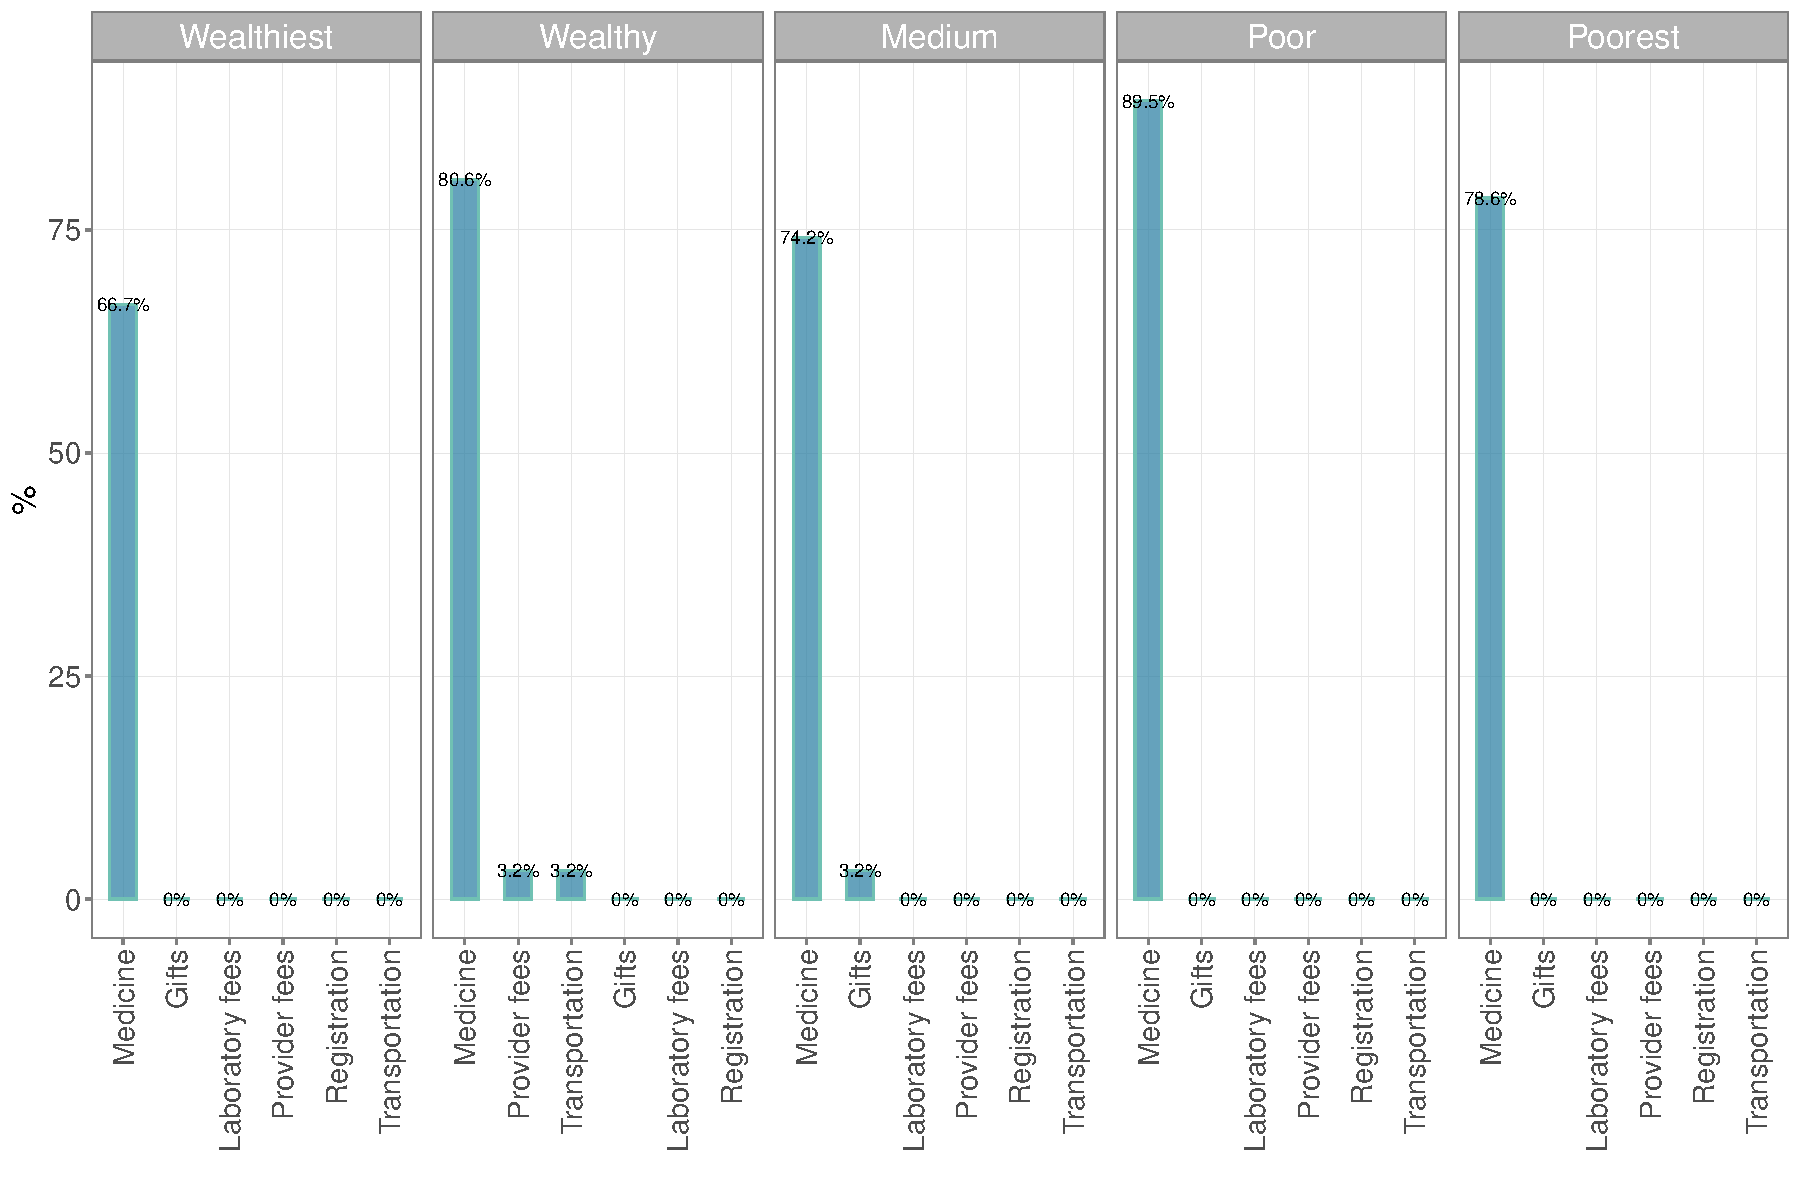
\includegraphics{kayahReport_files/figure-latex/fever8plot-1} 

}

\caption{Costs incurred for treatment in Kayah state}\label{fig:fever8plot}
\end{figure}

\hypertarget{study2-results}{%
\subsection{Cohort study}\label{study2-results}}

\newpage

\hypertarget{annex-1-study-questionnaires}{%
\section*{Annex 1: Study questionnaires}\label{annex-1-study-questionnaires}}
\addcontentsline{toc}{section}{Annex 1: Study questionnaires}

This goes here. What else?

\newpage

\hypertarget{annex-2-anthropometric-standardisation-results}{%
\section*{Annex 2: Anthropometric standardisation results}\label{annex-2-anthropometric-standardisation-results}}
\addcontentsline{toc}{section}{Annex 2: Anthropometric standardisation results}

Standardisation results here

\newpage

\hypertarget{annex-3-anthropometric-data-quality-check}{%
\section*{Annex 3: Anthropometric data quality check}\label{annex-3-anthropometric-data-quality-check}}
\addcontentsline{toc}{section}{Annex 3: Anthropometric data quality check}

\newpage

\renewcommand\refname{References}
\bibliography{bibliography.bib}


\end{document}
